%! TeX program = lualatex
\documentclass[a4paper,11pt,DIV=8]{scrbook}

\usepackage[english]{babel}

\usepackage{fontspec}
%\usepackage{amssymb}
% \usepackage[cmintegrals,cmbraces]{newtxmath}
% \usepackage{ebgaramond-maths}
\usepackage{mathtools}
\usepackage[math-style=ISO, bold-style=ISO]{unicode-math}
\setmathfont{Garamond-Math.otf}[StylisticSet={2,4,9}]

%\usepackage{mathastext}
%\usepackage[
%    subscriptcorrection,
%    nofontinfo,
%    mtphrd,
%    mtpfrak,
%    mtpcal,
%    zswash
%]{mtpro2}

%% Refs and Citations
\usepackage[
    backend=biber,
    backref=true,
    style=numeric-comp,
    %pagetracker=true,
    sorting=none,
    %comment=false,
    url=false,
    isbn=false,
    %doi=false
]{biblatex}
\addbibresource{bib/msc.bib}


\usepackage{enumitem}               % Ermöglicht verschiedene Aufzählungen (zb römisch)
\usepackage{textcomp}               
% \usepackage[onehalfspacing]{setspace}
\usepackage{tikz}
\usepackage{graphicx}		        
\usepackage{float}                  
\usepackage[font={small}]{caption}  

\usepackage{listliketab}
\usepackage{tabto}
\usepackage{isotope} 
\usepackage{extarrows}
\usepackage{booktabs}
\usepackage{capt-of}

%% Math & Physics QoL packages
\usepackage{amsmath}
\usepackage{amssymb}
\usepackage{amsthm}
\usepackage{bm}                 % access bold symbols in math mode
\usepackage{dsfont}
\usepackage{physics}
\usepackage{siunitx}
\usepackage{underoverlap}


\usepackage[colorlinks=true]{hyperref}
\usepackage[capitalize, noabbrev, nameinlink, english]{cleveref} 

\usepackage{lipsum}

\usepackage{titlesec}
\usepackage{epigraph}
\usepackage{geometry}
\usepackage{calc}
\usepackage{listings}

\usepackage{algorithm}
\usepackage{algorithmic}

\usepackage{xcolor}
\usepackage{tcolorbox}

% Load thesis.sty
\usepackage{./include/msc-thesis}


\setmainfont[scale=1]{EB Garamond}
\setsansfont[scale=0.9]{Libertinus Sans}
\setmonofont[scale=0.9]{Inconsolata}
%\setmathfont[range=bfsfit/{greek,Greek,latin,Latin,num}]{EB Garamond}


%%%%%%%%%%%%%%%%%%%
% THESIS METADATA %
%%%%%%%%%%%%%%%%%%%
\title{Cross entropy measures for detecting entanglement transitions}
\thesisname{Master's Thesis}
\author{Etienne Maurice Springer}
\university{Universität Stuttgart}
\date{27. November 2024}
\city{Stuttgart}
\institute{Institute for Theoretical Physics {III}}
\supervisor{Prof. Dr. Hans Peter Büchler}
\secondarycorrector{Prof. Dr. Maria Daghofer}

\hypersetup{
  colorlinks=true,
  linkcolor=maincolor5,
  citecolor=maincolor2,
  urlcolor=magma-40,
  linkbordercolor= {white},
  pdfauthor={Etienne Maurice Springer},
  pdfsubject={Master's Thesis},
  pdfpagelabels=true,
  breaklinks=true,
  plainpages=false,
  bookmarks, bookmarksnumbered=true
}

\graphicspath{{./fig/}}


%%%%%%%%%%%%%%%%%%%%%
% LISTINGS SETTINGS %
%%%%%%%%%%%%%%%%%%%%%

% The following is from NASA: 
% https://nasa.github.io/nasa-latex-docs/html/examples/listing.html

% Define a custom color
\definecolor{codegreen}{rgb}{0,0.6,0}
\definecolor{codegray}{rgb}{0.5,0.5,0.5}
\definecolor{codepurple}{rgb}{0.58,0,0.82}
\definecolor{backcolour}{rgb}{0.95,0.95,0.92}

% Define a custom lst style
\lstdefinestyle{myStyle}{
    backgroundcolor=\color{backcolour},   
    commentstyle=\color{codegreen},
    keywordstyle=\color{magenta},
    numberstyle=\tiny\color{codegray},
    stringstyle=\color{codepurple},
    basicstyle=\ttfamily\footnotesize,
    breakatwhitespace=false,         
    frame=single,
    breaklines=true,                 
    keepspaces=true,                 
    numbers=left,       
    numbersep=5pt,                  
    showspaces=false,                
    showstringspaces=false,
    showtabs=false,                  
    tabsize=2,
}

%%%%%%%%%%%%%%%%%
% CREF SETTINGS %
%%%%%%%%%%%%%%%%%
\crefname{thm}{Theorem}{Theorems}
\crefname{defn}{Definition}{Definitions}
\crefname{lem}{Lemma}{Lemmata} % or 'lemmata'?
\crefname{cor}{Corollary}{Corollaries} 
\crefname{conj}{Conjecture}{Conjectures}
\crefname{prop}{Proposition}{Propositions}
\crefname{alg}{Algorithm}{Algorithms}

%%%%%%%%%%%%%%%%%%%
% AMSTHM SETTINGS %
%%%%%%%%%%%%%%%%%%%
% Define a Style for tcolorbox Theorems and Definitions
\tcolorboxenvironment{thm}{
    colframe=black,
    colback=white!85!gray,
    boxrule=0.3mm,
    enhanced,
    borderline west={1mm}{0pt}{black},
    sharp corners,
}
\tcolorboxenvironment{defn}{
    colframe=black,
    colback=white!85!gray,
    boxrule=0.3mm,
    enhanced,
    borderline west={1mm}{0pt}{gray},
    sharp corners,
}
\tcolorboxenvironment{prop}{
    colframe=black,
    colback=white!85!gray,
    boxrule=0.3mm,
    enhanced,
    borderline west={1mm}{0pt}{gray},
    sharp corners,
}
\tcolorboxenvironment{lem}{
    colframe=black,
    colback=white!85!gray,
    boxrule=0.3mm,
    enhanced,
    borderline west={1mm}{0pt}{blue},
    sharp corners,
}
\tcolorboxenvironment{cor}{
    colframe=black,
    colback=white!85!gray,
    boxrule=0.3mm,
    enhanced,
    borderline west={1mm}{0pt}{red},
    sharp corners,
}
\theoremstyle{definition}
\newtheorem{thm}{Theorem}[chapter]
\newtheorem{defn}[thm]{Definition}
\newtheorem{lem}[thm]{Lemma}
\newtheorem{cor}[thm]{Corollary}
\newtheorem{conj}[thm]{Conjecture}
\newtheorem{prop}[thm]{Proposition}
\newtheorem{alg}[thm]{Algorithm}



%%%%%%%%%%%%%%%%%%
% TIKZ LIBRARIES %
%%%%%%%%%%%%%%%%%%

\usetikzlibrary{cd}
\usetikzlibrary{matrix}
\usetikzlibrary{shapes.geometric}
\usetikzlibrary{arrows}
%\usetikzlibrary{external}
%\tikzexternalize[prefix=fig/tikz/cache/]
%\tikzexternalenable

\tikzstyle{init} = [rectangle, minimum width=1cm, minimum height=.5cm, text
centered, text width=2.5cm, draw=black, fill=gray!20, font=\footnotesize]
\tikzstyle{timestep} = [gray, dashed]
\tikzstyle{measzz} = [rectangle, rounded corners, minimum width=3cm, minimum
height=1cm,text centered, draw=black, fill=blue!20]
\tikzstyle{errzz} = [rectangle, rounded corners, minimum width=3cm, minimum height=1cm, text
centered, draw=red, fill=red!30]
\tikzstyle{projzzsucc} = [rectangle, rounded corners, minimum width=3cm, minimum
height=1cm,text centered, draw=black, fill=green!15]
\tikzstyle{projzzfail} = [rectangle, rounded corners, minimum width=3cm, minimum
height=1cm,text centered, draw=black, fill=purple!15]
\tikzstyle{measx} = [rectangle, rounded corners, minimum width=1cm, minimum
height=1cm,text centered, draw=black, fill=blue!20]
\tikzstyle{errx} = [circle, minimum size=.1cm, text centered, draw=red, fill=red!30]
\tikzstyle{projxsucc} = [rectangle, rounded corners, minimum width=1cm, minimum
height=1cm,text centered, draw=black, fill=green!15]
\tikzstyle{projxfail} = [rectangle, rounded corners, minimum width=1cm, minimum
height=1cm,text centered, draw=black, fill=purple!15]

% for flowcharts (gepetto)
\tikzstyle{startstop} = [rectangle, rounded corners, minimum width=2cm, minimum height=1cm,text centered, draw=black, fill=red!30]
\tikzstyle{return} = [rectangle, minimum width=2cm, minimum height=1cm, text centered, draw=black, fill=orange!30]
\tikzstyle{process} = [rectangle, text width=8em, minimum width=2cm, minimum height=1cm, text centered, draw=black, fill=orange!30]
%\tikzstyle{decision} = [diamond, minimum width=2cm, minimum height=1cm, text centered, draw=black, fill=green!30]
\tikzstyle{arrow} = [thick,->,>=stealth]

% for flowcharts (latex forum)
\tikzstyle{decision} = [diamond, draw, fill=blue!20, 
    text width=6em, text badly centered, node distance=3cm, inner sep=0pt]
\tikzstyle{block} = [rectangle, draw, fill=blue!20, 
    text width=8em, text centered, rounded corners, minimum height=4em]
\tikzstyle{line} = [draw, -latex']
\tikzstyle{cloud} = [draw, ellipse,fill=red!20, node distance=3cm,
    minimum height=2em]

%\input{include/commands.tex}

\usepackage{layout}

\begin{document}
  
\KOMAoptions{twoside=false}
\makethesistitle
\KOMAoptions{twoside=true}

\frontmatter

\chapter{Abstract}
\label{ch:intro}

Random assortment of MIPT Paper (incomplete):
\begin{itemize}
  \item PTIM paper: \citetitle{langEntanglementTransitionProjective2020}
    \cite{langEntanglementTransitionProjective2020}
  \item Fisher paper, das ich mir als allererstes mal durchgelesen hab
    (\citetitle{liMeasurementdrivenEntanglementTransition2019}):
    \cite{liMeasurementdrivenEntanglementTransition2019}
  \item MIPT general, war in \cref{ch:lxe}, aber leider keine ahnung mehr
    warum\ldots (\citetitle{baoTheoryPhaseTransition2020}) \cite{baoTheoryPhaseTransition2020}
  \item Why not: Measurement induced synchronization von Finn
    (\citetitle{schmolkeMeasurementinducedQuantumSynchronization2023}):
    \cite{schmolkeMeasurementinducedQuantumSynchronization2023}
  \item 2017 WR for quantum state tomography (10 qubits):
    (\citetitle{song10QubitEntanglementParallel2017})
    \cite{song10QubitEntanglementParallel2017}
  \item LXE: Definition: \cite{liCrossEntropyBenchmark2023}; PTIM:
    \cite{tikhanovskayaUniversalityCrossEntropy2023}
  \item Garratt/Altman Paper:
    (\citetitle{garrattProbingPostmeasurementEntanglement2023}) \cite{garrattProbingPostmeasurementEntanglement2023}
  \item self-cite for clout:
    (\citetitle{schmolkeBoostingInformationTransfer2024})
    \cite{schmolkeBoostingInformationTransfer2024}
\end{itemize}

\lipsum[0-1]


\tableofcontents

\mainmatter

%\chapter*{}
\newpage
\layout*


%! TEX root = ../msc.tex
\chapter{Introduction}
\label{ch:basics}
\epigraph{I am fascinated by numbers}{
\citeauthor{baron-cohenAutismSpectrumQuotientAQ2001}}
%\cite{baron-cohenAutismSpectrumQuotientAQ2001}}

Was hier useful werden kann:

Nielsen: \cite{nielsenQuantumComputationQuantum2010}

Stabilizer Formalism, Gottesman PhD thesis: \cite{gottesmanStabilizerCodesQuantum1997}

Algorithm for simulating stabilizer circuits:
\cite{aaronsonImprovedSimulationStabilizer2004}

stabilizer lecture notes: \cite{arabLectureNotesQuantum2024}

Entanglement with Stabilizers: \cite{fattalEntanglementStabilizerFormalism2004}

Aaronson's quantum information theory I and II lecture notes:
\cite{aaronsonIntroductionQuantumInformation,aaronsonIntroductionQuantumInformationa}.
This one's a huge find!

another huge find! gottesman lecture notes on quantum error correction:
\cite{gottesmanSurvivingQuantumComputer2024}

Zee Group Theory in a nutshell: \cite{zeeGroupTheoryNutshell2016}

This chapter serves to familiarize the reader with the core concepts relevant
to this thesis. We will first introduce the stabilizer formalism, as it will
later enable us to perform efficient numerical experiments on a classical
computer. We then provide a general introduction to the field of entanglement
transitions and go over some important examples. 
\section{The Stabilizer Formalism}\label{sec:stab-basics}
In this section we review the most important concepts of the stabilizer
formalism. 

Section adapted from \cite{nielsenQuantumComputationQuantum2010} and
\cite{gottesmanStabilizerCodesQuantum1997}
\subsection{Basic notions of group theory}
Group theory is one of the most important algebraic notions in theoretical
phyiscs. From classifying crystalline structures (cite Ashcroft Mermin),
(gauge) symmetries in the standard model (cite some yang mills stuff), to the
classification of (topological) phase transitions (cite nicolai phd?), group
theory perpetually permeates theoretical physiscs.

The stabilizer formalism makes no exception. It is a clever application of
group theory, allowing for a more compact representation of quantum states,
compared to the state vector. We therefore introduce necessary prerequesites of
group theory needed for the stabilizer formalism and its role in this thesis,
starting with the notion of a group.

A group $G$ is a collection of some particulars $g$ that can be composed
according to some convention. To be called a group, the set of entities
$\{g\}$ and the operation\footnote{In the discussion on groups and group
  theory, the words composition, group operation, and multiplication are used
interchangibly} with which we compose them, need to obey a certain
ruleset. This ruleset, called the group axioms, reads as follows.

\begin{defn}[Group]\label{defn:group}
  A group $G$ is a non-empty set equipped with a binary operation (here denoted
  with $\cdot$) that satisfy
  \begin{description}
    \item[Associativity] The group operation is associative, i.e.
      $$\forall a,b,c \in G:\ (a\cdot b) \cdot c = a \cdot
      (b \cdot c)$$
    \item[Identity element] The group contains an identity element, which does
      nothing with respect to composition, i.e.
      $$\exists I\in G \ \forall g \in G : I\cdot g = g \cdot I = g$$
    \item[Inverse element] Each group element has a unique element associated
      to it that when composed with it gives the identity. In other words,
      $$\forall g \in G \ \exists g^{-1} \in G : g g^{-1} = g^{-1} g = I $$
  \end{description}
\end{defn}

Note that we do not require the group elements to commute with respect to
multiplication. Groups that satisfy commutativity for all their elements are
called \emph{abelian} groups.

Numerous different mathematical objects and concepts can fall under the
umbrella of group theory.\footnote{One can even describe the Rubik's Cube
puzzle in the language of group theory} Although we will discuss specific
groups in greater detail later, we do not want to fail to mention some other
important groups appearing all across physics. There are the rotation groups
$SO(n)$ and unitary groups $U(n)$ (both in $n$ dimensions), the permutation
group of $n$ elements $S_n$ and the group of square roots of $1$ under
multiplication, $\mathbb{Z}_2 = \{1, -1\}$.  The first two are examples of
continuous groups, while the others are discrete, meaning that they have a
finite number of elements. The number of elements in a discrete group $G$ is
called the \emph{order} of a group, which we write as $\mathrm{ord}(G)$.

For larger finite groups, it can become cumbersome to keep track of all the
elements and their relation to each other. Luckily, there is a way we can
condense all the information to construct the whole group in its
\emph{presentation}, also known as its \emph{generating set}. The elements of
such a generating set are referred to as \emph{generators}.
\begin{defn}[Generating set and generators]\label{defn:generators}
  Let $G$ be a finite group and $S$ a subset of $G$. $S$ is called a generating
  set of $G$ if all elements in $G$ can be obtained from (possibly repeated)
  multiplication of elements in the generating set. Generating sets are denoted
  by angled braces, such that we write
  \begin{align}
    S = \langle g_1, \ldots, g_n \rangle, \quad g_1,\ldots, g_n \in G
  .\end{align}
  The $g_i$ are called \emph{generators} of $G$. The trivial group $\left(
  \{I\}, \cdot \right)$ is generated by the empty set.
\end{defn}

While there are also generators of continuous groups, they take on a
fundamentally different form compared to the discrete counterpart. As an
example of a discrete generating set, consider the group of fourth roots of $1$
with multiplication, $Z_4 = \left( \{\pm 1,\pm i\}, \cdot \right)$. It is easy
to verify that the subset $S = \{i\}$ of the group uniquely reproduces all of
the elements in $Z_4$, by taking powers of $i$.

In the process of constructing a generating set we are generally faced with two
restrictions. The first is the fact that the entire group needs to emerge from
the multiplications of generators. We cannot simply choose arbitrary group
elements. $S=\{-1\}\subset Z_4$ would be a perfectly fine set of generators for
$\mathbb{Z}_2$, but not $Z_4$. Next, we ideally want to have the least number
of generators possible to build up the rest of the group. This restriction is
one we impose on ourselves rather than one imposed on us by necessity. Choosing
$S=\{-1, i, -i\}$ as generators also recovers $Z_4$, however, we have already
seen that $g=-1$ and $g=-i$ are redundant in this context.
\Cref{thm:maxsize-generators} gives a lower bound on the number of generators
needed to generate finite groups.

\begin{thm}\label{thm:maxsize-generators} 
  The minimum size of a generating set for a finite group $G$ of generators is
  at most $\log_2(\mathrm{ord}(G))$
\end{thm}

%\begin{proof} We prove the theorem by induction over the size of 
%
%  As base case we have Let $G$ be a finite group with minimal generating set
%  $S_n = \langle g_1, \ldots, g_n\rangle.$
%\end{proof}

With \cref{thm:maxsize-generators} we have that for $Z_4$, choosing a
generating set with $3$ elements should be cause for concern, since we would
need $2$ at most. However, we also saw that $Z_4$ is special in that way, since
we only needed one generator. A way of quantifying this quality is the
\emph{rank} of a group.  It is defined as the size of the smallest generating
set of $G$ and is denoted by $\abs{G}$. Thus, for the example of $Z_4$ we have
$\abs{Z_4}=1$. 
\newpage
When discussing subsets of groups, one naturally arising concept is the notion
of subgroups. Suppose we take some set of elements $\{g\}$ forming a group $G$
under multiplication and take a subset $\{h\}$ thereof. If the subset also
forms a group $H$, we call it a subgroup of $G$ and write $H \leq G$.

\begin{defn}[Subgroup]\label{defn:subgroup}
  A subgroup $H$ of $G$, written as $H \leq G$, is a non-empty subset $H$ of $G$, which forms
  a group under the same group operation as $G$. 
\end{defn}

Going back to some of the previous examples, we can consider $SO(2)$, rotations
along the unit circle, as rotations on the equator of a unit sphere. We can
consequently take $SO(2)$ as a subgroup of the rotation group of the unit
sphere $SO(3)$. The group of permutations of $m \leq n$ elements is just the
group of permutations of $n$ elements, where $n-m$ elements are left invariant,
and as such $S_m \leq S_n$. Note that for any group $G$ we have $G \leq G$ and
$(\{I\}, \cdot) \leq G$, where $\left( \{I\}, \cdot \right)$ is the trivial
group containing only the identity. These two special cases are referred to as
\emph{trivial subgroups}. Subgroups that are not trivial are called
\emph{proper subgroups} denoted by $H<G$.

Before introducing another important family of subgroups, we define a special
kind of operation known as \emph{conjugation}. If $h,g\in G$, the conjugate of
$h$ with respect to $g$ is $g^{-1} h g$.\footnote{This operation is
colloquially referred to as \enquote{sandwiching} $h$ with $g$.}
We can not only perform this operation on individual group elements, but also
subgroups of $G$. 
Consider the proper subgroup $H<G$ with elements $\{h_i\}$. 
%Another important family of subgroups are \emph{invariant} subgroups. Let $H$
%be a group of elements $\{h\}$ with $H<G$.
If we take any element $g \in G
\setminus H$, we can arrive at another subgroup of $G$ by conjugating all
elements of the
subgroup $H$ with $g$, written as
\begin{align}
  g^{-1}Hg = \{ g^{-1} h g \ \mid \ h \in H \}
.\end{align}
In general, the two subgroups $H$ and $g^{-1}Hg$ need not be the same. However,
if there are some $g$, which leave $H$ invariant under conjugation, we say that
these $g$ \emph{normalize} $H$. A collection of these normalizing elements can
be compiled together to form yet another subgroup of $G$, called the
normalizer.
\begin{defn}[Normalizer]\label{defn:normalizer}
  Let $G$ be a group and $H < G$ a proper subgroup of $G$. The normalizer of
  $H$ in $G$ is the subgroup of $G$ that leaves $H$ invariant under
  conjugation, i.e.
  \begin{align}
    N_G(H) = \{ g \in G \mid \ g^{-1} H g = H \}
  .\end{align}
\end{defn}
In the special case of every element of $G$ normalizing $H$, that is $N_G(H) =
G$, $H$ is called an \emph{invariant subgroup} of $G$. In the next section we
will introduce an important example of a finite group and its normalizer. 
%However,
%if, for an arbitrary choice of $g$, they are the same, then $H$ is called
%\emph{invariant subgroup} of $G$.
%\begin{defn}[Invariant subgroup]\label{defn:normal-subgroup}
%  Let $G, H$ be groups with $H\lt G$. We call $H$ an invariant (or normal)
%  subgroup of $G$ if
%  \begin{align}
%    \forall g \in G, \forall h \in H: \ g^{-1} h g \in H
%  .\end{align}
%\end{defn}
\subsection{The Pauli group and Clifford gates}

Consider the Pauli matrices with the identity,
\begin{align}
  \sigma_0 = I = \mqty(\pmat{0}),\quad \sigma_x = \mqty(\pmat{1}), \quad \sigma_y =
  \mqty(\pmat{2}), \quad \text{and}\quad \sigma_z = \mqty(\pmat{3})
.\end{align}
These well-known matrices are both hermitian and unitary, and consequently
square to the identity. For the latter three of them one can show that they
satisfy the following commutation and anticommutation relations,
\begin{equation}\label{eq:pauli-comm}
 \begin{split}
  [\sigma_j, \sigma_k] &= 2\mathrm{i}\epsilon_{jkl}\sigma_l \\
  \{\sigma_j, \sigma_k\} &= 2I \delta_{jk}\quad \text{and} \\
  \sigma_j \sigma_k &= \frac{1}{2}\left([\sigma_j,\sigma_k] +
  \{\sigma_j,\sigma_k\}  \right) = \delta_{jk} I + \mathrm{i} \epsilon_{jkl}
  \sigma_l
,\end{split} 
\end{equation}
with the Levi-Civita tensor $\epsilon_{jkl}$ (where Einstein summation
convention is implied) and the Kronecker delta $\delta_{jk}$. Furthermore, the latter
three are traceless and have eigenvalues of $\pm 1$.
To ease up on the
indices, especially once tensor products of Pauli matrices come into play, one also writes the Pauli matrix with the corresponding capital
letter, $\sigma_x = X, \ldots$. These matrices also form a basis for hermitian
$2\times 2$ matrices. Recall that physical observables are represented by
hermitian matrices. We can therefore consider the Pauli matrices as a basis for
physical observables on qubits. 

While they also play
an important role in representation theory, especially of Lie and Clifford
algebras, they themselves also form a group known as the Pauli group
$\mathcal{P}$. The single-qubit Pauli group is defined as the Pauli matrices
with phases $\pm 1$ and $\pm i$,
\begin{align}
  \mathcal{P} = \{\pm I, \pm i I, \pm X, \pm i X, \pm Y, \pm i Y, \pm Z, \pm i
  Z \}
.\end{align}
This definition can also be generalized to $n$ qubits.
\begin{defn}[Pauli group]\label{defn:pauligroup}
  The Pauli group $\mathcal{P}_n$ is composed of tensor products of $I,\ X,\
  Y,$ and $Z$ on $n$ qubits with an overall phase of $\pm 1$ and $\pm i$.
\end{defn}
From \cref{eq:pauli-comm} it follows that $\mathcal{P}_n$ is not Abelian.
The commutation relations can be extended for the tensor products of Paulis,
but there are some cases that then commute non-trivially. For instance,
$X_1\otimes X_2 \equiv X_1X_2$ commutes with $Z_1\otimes Z_2\equiv Z_1Z_2$, even though the individual
Pauli matrices in the tensor products do not commute. These commutation
relations can be compacted into a general statement on tensor products of Pauli
operators. Two $n$-qubit Pauli operators commute non-trivially if there are an
even number of anticommuting pairs in the tensor product structure. This
excludes the identity, of course, since everything commutes trivially with the
identity. The task of finding the commutation relation between two operators
then becomes a counting task.

Another group worth considering is the Clifford group, $\mathsf{C}_n$, which is
often defined as the subgroup of unitary matrices with dimension $2^n$ that
normalize (cf. \cref{defn:normalizer}) the $n$-qubit Pauli group,
$$\mathsf{C}_n = \{ u \in U\left(2^n\right) \mid u^\dagger \mathcal{P}_n u
= \mathcal{P}_n \}.$$
Instead of being a finite group, since it includes all matrices of the form
$u= e^{i\varphi} I$ with some phase $\varphi \in \mathbb{R}$, the Clifford
group defined in this way is continuous. By defining it in terms of a finite
subgroup of the above definition, the physical significance of the Clifford
group also becomes apparent.

\begin{defn}[Clifford gates]\label{defn:cliffords}
  The Clifford group is the group generated by the Hadamard, Phase and CNOT
  gates. These are called the Clifford gates. 
\end{defn}

The Clifford gates form an important subset of gates in quantum computing and
especially quantum error correction (\textcolor{orange}{hier ein paar citations
vielleicht}). However, it should be noted that they do not form a universal set
of quantum gates. While the gates in the Clifford group can create entangled
states with the Hadamard and CNOT gates, one needs an additional gate to
achieve universal quantum computation.
\subsection{The stabilizer group}

So far we have only examined groups in isolation. Among other things, we have
shown that the group generated by the Clifford gates normalizes the Pauli
group.  However, the major role group theory plays in physics can best be
demonstrated if one considers the action of group elements on other
mathematical objects outside of the group. These could be, for example,
Lagrangians, or more relevant for us, state vectors. If we consider the
two-qubit state vector $\ket{+} = \left( \ket{0} + \ket{1} \right) / \sqrt{2}$.
As an eigenstate of the Pauli operator $X$, we can tell that this state is
resistant to bitflips.  The group-theoretic way to put this is to say that
$\ket{+}$ is $\mathbb{Z}_2$-symmetric. This notion of symmetry is where group
theory finds most of its utility in physics.  As an additional example,
consider the 2-qubit Bell state

\begin{align}
  \ket{\phi} = \frac{\ket{00} + \ket{11}}{\sqrt{2}} 
.\end{align}

Note that the unitary operations $X_1 X_2$ and $Z_1 Z_2$ both have $\ket{\phi}$
as eigenstate with eigenvalue $+1$. Since $$X_1X_2Z_1Z_2\ket{\phi} = \ket{\phi} =
Z_1Z_2X_1X_2\ket{\phi}$$ we can also see how these two operators commute with each
other. The operators $X_1X_2$ and $Z_1Z_2$ are then said to \emph{stabilize} the
state $\ket{\phi}$. It is easy to convince oneself that these operations
stabilizing the state $\ket{\phi}$ should form a group. Doing nothing, i.e. the
identity $I$, clearly stabilizes the state, and since the Pauli matrices square
to the identity, each element of this stabilizer group is its own inverse (we
omit verifying associativity, as this is inherited from $\mathcal{P}_n$). The
matrices $X_1X_2$ and $Z_1Z_2$ therefore generate a symmetry group of
$\ket{\phi}$, since their product is clearly also a symmetry transformation on
$\ket{\phi}$. We therefore introduce the final group theoretic notion, the
symmetry group.

\begin{defn}[Symmetry group]\label{defn:fixpointgroup}
  Let $G$ be a group acting on a set $M$. Let $a\in M$. We then call the
  subgroup
  \[ H = \left\{ h \in G \mid ha = a \right\} \leq G \]
  \emph{symmetry group} or \emph{fixpoint group} of $a$.
\end{defn}

In our example, we have the group of $2$-qubit Pauli matrices, $\mathcal{P}_2$,
acting on the $2$-qubit Hilbert space $H^{\otimes 2}$.
%The symmetry group of
%$\ket{\phi} \in H^{\otimes 2}$ is the subgroup of Pauli matrices that have the
%state as eigenvector with eigenvalue $+1$. 
In general, we say that a unitary $U$ stabilizes a pure state $\ket{\psi}$ if
$U\ket{\psi} = \ket{\psi}$. In other words, the stabilizer group of a pure
state
$\ket{\psi}$ is the set of all unitaries that have $\ket{\psi}$ as eigenvector
with eigenvalue $+1$. For all further considerations we restrict the unitaries
to Pauli operators. Thus, the formal definition of an $n$-qubit stabilizer
group can be stated as follows.

\begin{defn}[Stabilizer group]\label{defn:stabilizergroup}
  Let $H^{\otimes n}$ denote the $n$-qubit Hilbert space. Given a subset $V_S
  \subseteq H^{\otimes n}$, the stabilizer is defined as
  \begin{align}
    \mathcal{S}_V = \{ g \in \mathcal{P}_n \mid g \ket{\phi} = \ket{\phi} \
    \forall \ket{\phi} \in V \} \leq \mathcal{P}_n
  .\end{align}
\end{defn}

It would, in principle, be possible to define stabilizer groups of all
unitaries instead of the Pauli group. We will later see, however, that this
restriction leads to an important result, namely \cref{thm:gottesman-knill}.

We note that global phase matters here. The operators with prefactor, such as
$-I$ are not in the stabilizer. Furthermore, we have that the stabilizer is an
Abelian subgroup of $\mathcal{P}_n$, which can be shown by generalizing the
example above. We can show the necessity of this condition in the following.
Suppose $\ket{\phi}\in V_S$ is non-zero, and $M$ and $N$ are in $\mathcal{S}$. Since $M$
and $N$ are tensor products of Pauli matrices, they either commute or
anticommute. If they anticommute we have
\begin{align}
  \ket{\phi} = MN\ket{\phi} = -NM\ket{\phi} = -\ket{\phi}
,\end{align}
leading to a contradiction, since we had $\ket{\phi}$ being non-zero. (By the
same argument we can rule out $-I$ to be in the stabilizer.)

At this point, we need to be careful not to put the cart before the horse. The stabilizer
group is not the stabilizer of $V_S$ as such. If that were the case, then $V_S
= \{ \ket{00}, \ket{11}\}$ would be stabilized by $X_1X_2$. Rather, $V_S$ is
the intersection of subspaces spanned by the eigenvalue $+1$ eigenspaces of 
$\mathcal{S}$. What this means is that when working with the stabilizer formalism, we would
much rather first write out an Abelian subgroup of the Pauli group (without
$-I$) and then
deduce the subspace stabilized by this subgroup. 

\begin{defn}[Stabilized state space]\label{defn:stab-statespace}
  Let $\mathcal{S} \leq \mathcal{P}_n$ be Abelian with $-I \not\in
  \mathcal{S}$. The space of states stabilized by $\mathcal{S}$ is
  \begin{align}
    V_S = \{ \ket{\phi} \mid g\ket{\phi} = \ket{\phi} \ \forall g \in
    \mathcal{S} \}
  .\end{align}
\end{defn}

So far, it is not entirely obvious how keeping track of operators growing
exponentially in size is a worthwhile method of representing quantum states or
subspaces of a larger state space.
However, we can simplify the problem drastically by realizing two facts.

The first is summarized in \cref{defn:generators,thm:maxsize-generators}.
Recall that we can equivalently write a finite group as a collection of at most
$\log(\mathrm{ord}(G))$ generators. The Bell state example from above has a
full stabilizer group of $\mathcal{S} = \{I, X_1X_2, -Y_1Y_2, Z_1Z_2\}$. With
\cref{eq:pauli-comm} we can infer that $X_1X_2\cdot Z_1Z_2 = -Y_1Y_2$, and
since all of them square to the identity, an equivalent form of the stabilizer
group is given by the generating set $G = \langle X_1X_2, Z_1Z_2\rangle$.
Note that while the generating set is explicitly not the entire group, the
distinction between the two is kept rather loosely. Oftentimes we will write
that some stabilizer group $\mathcal{S}$ is equal to its generating set. This is mostly a matter of
convenience and reabability. If context does not explicitly demand it, we write
the generating set and the group interchangibly.

The second fact is a more subtle one. It uses the commutation relations
laid out in \cref{eq:pauli-comm}. If we briefly neglect the phases again, or keep
track of them separately, we can write $Y=XZ$. As such, we can encode the
entire stabilizer group in a bit matrix, where $I \equiv 00$, $Z \equiv 01$, $X
\equiv 10,$ and $Y \equiv 11$. The bit matrix of the Bell state is
\begin{align}
  \mathcal{S} \equiv \mqty[1 & 1 & 0 & 0 \\ 0 & 0 & 1 & 1]
.\end{align}
This check matrix has a multitude of different use cases, one of them being the
focus of the entirety of \cref{ch:mixed}.
Another one is that if the rows of the
check matrix are linearly independent (mod 2), we have a minimal generating
set. The generators of such a minimal generating set are then called
independent. 

\subsubsection{Stabilizer density matrix}
Before we go on to discuss the dynamics in the stabilizer formalism, i.e.
stabilizer circuits, we define the density matrix for stabilizers. We know that
a stabilizer group $\mathcal{S}$ consists of Pauli operators, which share eigenstates. 
Thus, the density matrix of a pure state $\rho = \dyad{\phi}$ is a
projector onto all $+1$ eigenstates of the Pauli operators in the stabilizer.
This can be constructed by multiplying the projectors onto $+1$ eigenstates of
the generating set. This follows from $\mathbb{P}^2 = \mathbb{P}$ and the fact
that the generating set recovers the whole group with multiplication. Since we
can write projectors of Pauli operators $g$ as $\mathbb{P} = \frac{1}{2}(I+g)$,
we can write
\begin{align}
  \rho = \frac{1}{2^n} \prod_{i=1}^n (I + g_i)
\end{align}
for the density matrix of a pure state.

A mixed state in the stabilizer formalism can be described by removing
generators from the generating set. 
\begin{defn}[Stabilizer density matrix]\label{defn:stab-dmat}
  Let $\mathcal{S}$ be an $n$-qubit stabilizer group with generating set
  $\langle g_1, \ldots, g_l \rangle$ with $0 \leq l \leq n$. The density matrix
  corresponding to this stabilizer group is given by
  \begin{align}
    \rho = \frac{1}{2^n} \prod_{i=1}^l (I + g_i)
  \end{align}
  or alternatively as
  \begin{align}
    \rho = \frac{1}{2^n} \sum_{s \in \mathcal{S}} s
  .\end{align}
\end{defn}

\subsubsection{Entropy of entanglement}

With the notion of a density matrix defined in the stabilizer formalism, we can
ask the question about entropic quantities. Since we introduce methods to
compute other entropic and information-theoretic quantities in
\cref{sec:rel-ent-stab}, we will here only define the entropy of entanglement.
Its definition can be stated as follows.
\begin{defn}[Entropy of entanglement]\label{defn:entent}
  Let $\ket{\phi}\in H^{\otimes N}$ be a bipartite pure state with subsystems
  $A$ and $B$. The entropy of entanglement of $\ket{\phi}$ then reads
  \begin{align}
    %&S_E : H^{\otimes N} \to [0, N/2]\nonumber\\
    S_\mathrm{E}\left(\ket{\phi}\right) = - \Tr[\rho_B \log \rho_B],
  \end{align}
  where $\rho_B = \Tr_A[\dyad{\phi}]$ is the reduced density matrix of subsystem
  $B$. Conventionally, one uses the logarithm of base 2.
\end{defn}

In bipartite states this quantity measures how entangled one subsystem is with
the other. That is, it gives a numerical value to the non-local correlations between
subsystems. If we split our stabilizer group into local subgroups of $A$ and
$B$, $\mathcal{S}_A$ and $\mathcal{S}_B$, we have the possibility of another
subgroup remaining, namely $\mathcal{S}_{AB}$ accounting for correlations.
$\mathcal{S}_{A(B)}$ are subgroups containing only operators acting on $A (B)$.
If we split our stabilizer group in this way, we find that there is a nice
closed-form expression for the entanglement entropy
\cite{fattalEntanglementStabilizerFormalism2004}.

\begin{thm}[Entropy of entanglement -- stabilizer]\label{thm:entent}
  The entropy of entanglement of a bipartite pure state $\ket{\phi}_{AB}$ with
  partitions $A$ and $B$ is given
  by
  \begin{align}\label{eq:entent}
    S_E(\ket{\phi}) = \frac{1}{2}\abs{\mathcal{S}_{AB}}
  .\end{align}
\end{thm}
For
the 2-qubit Bell state we once again have $\mathcal{S} = \langle XX,
ZZ\rangle$. Notice that $\mathcal{S}_A = \mathcal{S}_B = \{I\}$ and $\mathcal{S}_{AB} =
\mathcal{S}$. 
The entropy of entanglement between $A$ and $B$ should be $1$
since there is only 1 independent entangled pair. We could additionally compute
the reduced density matrices and the matrix logarithm instead, arriving at the
same result.

With \cref{eq:entent} we find that this result is also obtained by counting the
generators in $\mathcal{S}_{AB}$, which is $2$, then dividing by $2$, which
gives the correct result of $1$. 
\subsection{Stabilizer circuits}

Finally, we discuss the dynamics of stabilizer states in quantum circuits. This
is where we can see the main advantages of the stabilizer formalism, as it will
ultimately lead to the efficient simulation of a wide class of quantum circuits
with classical computers. 
As introductory note we define a stabilizer circuit to be a quantum
circuit using only Clifford gates and measurement gates of Pauli operators. Let
us therefore begin by discussing unitary gates.

\subsubsection{Unitary gates}
Suppose we apply a unitary $U$ to a vector space $V_S$ stabilized by
$\mathcal{S}$. For any $\ket{\phi} \in V_S$ and any $g \in \mathcal{S}$ we have
\begin{align}
  U\ket{\phi} = U g \ket{\phi} = U g \underbrace{U^\dagger U}_{I} \ket{\phi}
.\end{align}
We thus have that the state $U\ket{\phi}$ is stabilized by the operator
$UgU^\dagger$. Since our choices of $\ket{\phi}$ and $g$ were arbitrary in
$V_S$ and $\mathcal{S}$, respectively, we have that the transformed vector
space is stabilized by the conjugated stabilizer group
\begin{align}
  USU^\dagger = \{ UgU^\dagger \mid g \in \mathcal{S}\}
.\end{align}
Since we restricted ourselves to unitary gates in the Clifford group, which
normalizes the Pauli group, we still exclusively have Pauli operators in
$USU^\dagger$. Our task then becomes to track the effects of Clifford group
elements on a subset of Pauli operators. In particular, we conjugate the
generators in the generating set with the unitary operation corresponding to
the applied gate. Let us therefore consider the
conjugation of the Pauli matrices with the unitary Clifford gates.
For the Hadamard gate $H = \frac{X+Z}{\sqrt{2}}$ we have
\begin{align}
  HXH^\dagger = Z, \quad HYH^\dagger = -Y, \quad HZH^\dagger = X
\end{align}
For the CNOT gate $U$ with qubit 1 as control and qubit 2 as target we have
\begin{alignat}{2}
  UX_1U^\dagger &= X_1X_2, \quad &&UX_2U^\dagger = X_2 \label{eq:cnot-x}\\
  UZ_1U^\dagger &= Z_1, \quad &&UZ_2U^\dagger = Z_1Z_2
,\end{alignat}
where for all other two qubit Pauli operators we can use the above relations
and \cref{eq:pauli-comm} to
deduce their conjugation relations. Furthermore, we already know an efficient method
of tracking generating sets through $X$ and $Z$ alone.
Lastly, we want to consider the action of the phase gate on the Pauli
operators,
\begin{align}
  SXS^\dagger = Y \quad SZS^\dagger = Z
.\end{align}

Note that the Clifford gates being the normalizer of the Pauli group means that
we will inevitably lose gates, which would realize universal quantum computing.
Notable examples of gates not included in the gate set generated by the
Clifford group are the $T$ gate, also known as $\pi /8$ gate, and the Toffoli
gates.

\subsubsection{Measurements}

We now know the mechanisms behind unitary gates in the stabilizer formalism.
However, we can also include measurement gates in quantum circuits. It turns
out that measurements can also be described in a simple way in the stabilizer
formalism. Since physical observables are represented by hermitian operators,
we can assume that the measurement operator is a product of Pauli matrices $M
\in\mathcal{P}_n$. Suppose we measure $M$ in a system in a state $\ket{\phi}$
with stabilizer group $\mathcal{S} = \langle g_1, \ldots, g_n\rangle$. Two
questions naturally arise: what is the measurement result, and how does the
stabilizer group transform under this measurement?

To answer both of these, we first need to realize the two distinct
possibilities:
\begin{enumerate}
  \item $M$ commutes with all the generators of the stabilizer group.
  \item $M$ anti-commutes with at least one of the generators. By restructuring
    the generating set, we can ensure that there is at most one generator
    anticommuting with $M$. We thus assume without loss of generality that $M$
    anticommutes with $g_1$.
\end{enumerate}

For the first case, we have that either $M$ or $-M$ is itself an element of the
stabilizer group, since for arbirtary generators $g_j$
\begin{align}
  g_j M \ket{\phi} = M g_j \ket{\phi} = M\ket{\phi}
.\end{align}
As this holds for any $g_j$, we have that $M\ket{\phi}=\pm \ket{\phi}$, where
either $\pm M$ is in the stabilizer group. Assuming w.l.o.g. that
$M\in\mathcal{S}$, we have that the measurement of $M$ yields the result $+1$
with probability one, i.e. deterministically. Since the stabilizer group
already contained $M$, it does not change. 

In the second case, we have that the measurement operator anticommutes with
$g_1$. Note that the projectors for the measurement outcomes are $\mathbb{P} =
\frac{1}{2}\left( I\pm M \right)$. Therefore, the probabilities for the
respective outcomes are given by
\begin{align}
  P(\pm 1) = \Tr[\frac{1}{2}\left( I\pm M \right) \dyad{\phi}]
.\end{align}
With $g_1 \ket{\phi} = \ket{\phi}$ and $\{g_1, M\} =0$ we have
\begin{align}
  P(+1) &= \Tr[\frac{I+M}{2} g_1 \dyad{\phi}] \nonumber\\
        &= \Tr[g_1 \frac{I-M}{2} \dyad{\phi}] \nonumber\\
        &= \Tr[\frac{I-M}{2} \dyad{\phi} g_1] \nonumber\\
        &= \Tr[\frac{I-M}{2} \dyad{\phi}] = P(-1)
.\end{align}
Since we can only measure $+1$ or $-1$ and the probabilities for either are
equal, we can deduce that $P(\pm 1) = 1 / 2$. After the measurement, the
generating set gets affected such that it is now
$\rangle \pm M, g_2, \ldots, g_n\rangle$ depending on the measurement outcome.

\subsubsection{Stabilizer circuits and error correction}

No discussion of the stabilizer formalism would be complete without as much as
a mention of its applications in quantum error correction. To this end,
consider the following quantum circuit shown in
\cref{fig:error-detection-circuit}. A variation of this circuit will play
an important role in our discussion of the projective transverse-field Ising
model in \cref{sec:intro-ptim}.

\begin{figure}[H]
  \centering
  \begin{quantikz}
  \lstick{$\ket{0}$} & \gate{H} & \ctrl{1} & \ctrl{2} & &\meter[2]{$ZZ$} & \\
  \lstick{$\ket{0}$} & & \targ{} & & & & \meter[2]{$ZZ$} \\
  \lstick{$\ket{0}$} & & & \targ{} & \meter[style={fill=red!20}]{$X$} & &
\end{quantikz} 

  \caption{Circuit showing the error detection and correction capabilities
    within the stabilizer formalism.  First, a Bell cluster is created by the
    application of the Hadamard and two CNOT gates.  Afterwards, an error
    occurs in the form of an $X$ measurement, which we can attempt to detect
    via stabilizer measurements.}
  \label{fig:error-detection-circuit}
\end{figure}

Initially, we have the state $\ket{000}$, which is stabilized by $\mathcal{S} =
\langle Z_1, Z_2, Z_3 \rangle$. At the first vertical line our generators were
conjugated with $H_1$, such that we now have $\mathcal{S} = \langle X_1, Z_2,
Z_3 \rangle$. The corrresponding state stabilized by $\mathcal{S}$ is
$\ket{+}\otimes\ket{00}=\frac{\ket{0}+\ket{1}}{\sqrt{2}} \otimes \ket{00}$.
After the first CNOT, we have $\mathcal{S} = \langle X_1X_2,Z_1Z_2,Z_3\rangle$
according to the transformation rules given in \cref{eq:cnot-x}. Before the measurement on qubit 1, we
apply another CNOT gate, thus creating a 3-qubit Bell cluster
$(\ket{000}+\ket{111}) / \sqrt{2}$ with stabilizer group $\mathcal{S}= \langle
X_1X_2X_3,Z_1Z_2,Z_2Z_3\rangle$. 

Then, an error occurs in the form of an $X$ measurement on qubit 3. The
stabilizer generators are now $\langle X_1X_2, Z_1Z_2, X_3\rangle$, which we
are, in principle, unaware of. However,
since we are performing syndrome measurements afterwards in the form of $ZZ$
measurements, we can detect, and subsequently correct the error. In our
example, a measurement of $Z_1Z_2$ would be a measurement of a stabilizer
generator, and would thus yield $+1$. Next, we measure $Z_2Z_3$. According to
the previously introduced rules, the outcome is $\pm 1$ with probability
$\frac{1}{2}$ and the stabilizer generators afterwards are $\mathcal{S} =
\langle X_1X_2X_3, Z_1Z_2, \pm Z_2Z_3\rangle$. In the case where the outcome is
$+1$, we effectively corrected the error already, since we recovered the
previous stabilizers. In the converse case, we at least detected the syndrome
of the error: bit flip on qubit $3$ must have occurred! We can then correct the
error appropriately and flip it back by means of applying a Pauli-$X$.
%We then measure the first qubit in the
%computational basis. We have that $\{Z_1,X_1\} = 0$, and thus a random outcome
%to the measurement. However, after the measurement we are guaranteed to have
%stabilizers in the form of $\mathcal{S} = \langle \pm Z_1, Z_1Z_2,
%Z_2Z_3\rangle$.

\subsubsection{Simulation of stabilizer circuits}
Simulating stabilizer circuits can thus be done by keeping track of all the
generators and updating them accordingly. As we have seen in above example, we
were not required to perform exponentially hard calculations to get to the
final state of the circuit. This fact can be used to formulate the following
theorem \cite{gottesmanHeisenbergRepresentationQuantum1998}.
%Currently verbatim from \cite{nielsenQuantumComputationQuantum2010}! Beware!
%Actual source is \emph{inside}
%\cite{gottesmanHeisenbergRepresentationQuantum1998}, basically stating "trust
%me bro" (one of the most important theorems of quantum computation is cited as
%private communication in its original source\ldots)
\begin{thm}[Gottesman-Knill theorem]\label{thm:gottesman-knill}
  Suppose a quantum computation is performed which involves only the following
  elements: state preparations in the computational basis, Clifford gates, and
  measurements of observables in the Pauli group (which includes measurement in
  the computational basis as a special case), together with the possibility of
  classical control conditioned on the outcome of such measurements. Such
  computation may be efficiently simulated on a classical computer.
\end{thm}

We will forego a detailed discussion of the simulation of stabilizer circuits
on classical computers, as well as the proof to \cref{thm:gottesman-knill}
until \cref{ch:mixed}. For now we remind ourselves that the Clifford gate set
does not constitute a universal set of quantum gates. Thus, classical computers
\emph{cannot} suffice to efficiently simulate quantum computers

\section{Entanglement Transitions}\label{sec:ent-trans}

Random assortment of MIPT Paper (incomplete):

\begin{itemize}
  \item Fisher paper, das ich mir als allererstes mal durchgelesen hab
    (\citetitle{liMeasurementdrivenEntanglementTransition2019}):
    \cite{liMeasurementdrivenEntanglementTransition2019}
  \item MIPT general, war in \cref{ch:lxe}, aber leider keine ahnung mehr
    warum\ldots (\citetitle{baoTheoryPhaseTransition2020}) \cite{baoTheoryPhaseTransition2020}
  \item \citetitle{baoSymmetryEnrichedPhases2021}
    \cite{baoSymmetryEnrichedPhases2021}
  \item Why not: Measurement induced synchronization von Finn
    (\citetitle{schmolkeMeasurementinducedQuantumSynchronization2023}):
    \cite{schmolkeMeasurementinducedQuantumSynchronization2023}
  \item 2017 WR for quantum state tomography (10 qubits):
    (\citetitle{song10QubitEntanglementParallel2017})
    \cite{song10QubitEntanglementParallel2017}
  \item LXE: Definition: \cite{liCrossEntropyBenchmark2023}; PTIM:
    \cite{tikhanovskayaUniversalityCrossEntropy2023}
  \item Garratt/Altman Paper:
    (\citetitle{garrattProbingPostmeasurementEntanglement2023}) \cite{garrattProbingPostmeasurementEntanglement2023}
  \item self-cite for clout:
    (\citetitle{schmolkeBoostingInformationTransfer2024})
    \cite{schmolkeBoostingInformationTransfer2024}
\end{itemize}

more curated MIPT collection:
\begin{itemize}
  \item Skinner Lecture notes on MIPT
    \cite{skinnerLectureNotesIntroduction2023}
  \item ist zwei mal in meiner zotero library, vielleicht mal auschecken: 
    \cite{hokeMeasurementinducedEntanglementTeleportation2023}
  \item Titel klingt vielversprechend: \cite{baoTheoryPhaseTransition2020}
  \item Ideen von Finn: \cite{joshiObservingQuantumMpemba2024,aresEntanglementAsymmetryProbe2023}
  \item PRX von skinner 1: \cite{skinnerMeasurementInducedPhaseTransitions2019}
    chronologisch das erste
  \item PRX von skinner 2: \cite{nahumMeasurementEntanglementPhase2021}
  \item PRX von skinner 3:
    \cite{nahumEntanglementDynamicsDiffusionannihilation2020}
    Das hat Felix immer auf gemacht um mir das mit den Majoranas zu zeigen
  \item eins noch for good measure:
    \cite{yoshidaDecodingEntanglementStructure2021}
\end{itemize}
\begin{figure}[H]
  \centering
  
\includegraphics{Untitled.png}
  \caption{Hybrid Circuit Tikz picture??}
  \label{fig:hybrid-circuit}
\end{figure}

\subsection{Phenomenology}

\section{The Projective Transverse-Field Ising Model}\label{sec:intro-ptim}
\begin{itemize}
  \item PTIM paper: \citetitle{langEntanglementTransitionProjective2020}
    \cite{langEntanglementTransitionProjective2020}
  \item Felix decoder paper: \citetitle{roserDecodingProjectiveTransverse2023}
    \cite{roserDecodingProjectiveTransverse2023}
  \item Colored Cluster Model!
  \item There should be a Skinner paper, but I don't have it in my zotero
    library (yet)
  \item Its \cite{nahumEntanglementDynamicsDiffusionannihilation2020}
\end{itemize}
\begin{figure}[H]
  \centering
  \begin{tikzpicture}
  \draw[gray, dashdotted, xstep=1cm, ystep=1cm] (0,0) grid (10,10);
\end{tikzpicture}

  \caption{Tikz sketch of PTIM setup with $\approx 10$ qubits}
  \label{fig:ptim-circuit}
\end{figure}
\begin{figure}[H]
  \centering
  
\includegraphics{Untitled.png}
  \caption{Tikz sketch of PTIM setup with $\approx 10$ qubits}
  \label{fig:ptim-circuit}
\end{figure}

\begin{figure}[H]
  \centering
  
\includegraphics{Untitled.png}
  \caption{plot of entanglement entropy (and mutual information??) as a
  function of $p$. multiple system sizes, possibly rather large ($\approx 512$
qubits?, maybe $N=\{128,256,512\}$ just for the fun of it). Would need to
include mutual information in the source code.}
  \label{fig:phase-transition}
\end{figure}

\section{Sampling Problem}\label{sec:sampling}
The metaphysics of this endeavour can
be condensed in the following way; we (a) know from experiments how quantum
systems behave under certain conditions, and (b) predict through theoretical
calculations what these systems might do in another experimental setting. In
the latter case however, there is an uncanny regime of utility, where we either
(a) cannot precisely pass predictions or (b) cannot perform the experiment on
the grounds of hardware limitations\footnote{The Higgs particle was predicted
40 years before it was discovered \textcolor{red}{citation}} or (c) try to
predict the behavior of quantities not directly measurable. In the case of
quantum computation, and especially in the field of entanglement transitions,
we face these bottlenecks in increasing severity. To make do with them, we
employ classical computer simulations. That is, we perform numerical
experiments. While traditional experiments still serve as the sole proprietor of claim to
ontology, numerical experiments can play a supporting role, 

In the year of our
lord 2024, we phyisicists are thankfully able to perform experiments at home
with cleverly assembled silicon.  That is, nowadays we make do with these
bottlenecks by performing numerical experiments. This is not to discredit the
utility of experiments as such, on the contrary! 

\subsection{Fisher: Linear Cross Entropy}
\cite{liCrossEntropyBenchmark2023}

\subsection{Altman: Upper Bound}
\cite{garrattProbingPostmeasurementEntanglement2024}


\chapter{Linear Cross Entropy}
\label{ch:lxe}
\epigraph{Check the circuit}{Spock to helmsman;
  \citefield{butlerCage1988}{booktitle}
--- \citefield{butlerCage1988}{number}}

PTIM: \cite{langEntanglementTransitionProjective2020}

Fisher/Altman PRL, hier wird die LXE definiert: \cite{liCrossEntropyBenchmark2023}

Nicolai: \enquote{Das ist eines der Paper, die Fisher zitiert, wo die LXE eingeführt wurde.} \cite{baoSymmetryEnrichedPhases2021}

arXiv:2306.00058, LXE fürs PTIM, preprint \cite{tikhanovskayaUniversalityCrossEntropy2023}

MIPT allgemein, hier leider eher weniger ahnung warum ich das in dieses Kapitel rein
gemacht hab zum zitieren. \cite{baoTheoryPhaseTransition2020}

Sampling stuff aus appendix von \cite{roserDecodingProjectiveTransverse2023}

\section{WIP: Definition and properties}
Before stating the definition of the linear cross entropy, we will first
introduce some notational conventions.

Suppose we run a PTIM simulation on some platform, either classically with
stabilizer circuits or on a quantum simulator. The system is initially in some
state $\rho$ and will subsequently be subjected to local projective $X$ and
$ZZ$ measurements.  After having applied the circuit on $\rho$, we find
ourselves with recorded measurement outcomes. We write $\mathbf{m}$ for the
mathematical object representing this measurement record. It can be
thought of as a vector of all outcomes in order of recording.
Since quantum measurements are generally probabilistic, any full
measurement record $\mathbf{m}$ might contain an arbitrary number of outcomes
$m$ with probability $0\leq P(m=\pm 1 | C, \rho)\leq 1$. A given
measurement pattern therefore has many possible records, each with some
probability.  We write this probability of a measurement record $\mathbf{m}$
given a measurement pattern $C$ and an initial state $\rho$ as $P(\mathbf{m}
\mid C, \rho)$. As we specifically investigate the PTIM, our measurement record
$\mathbf{m}$ can equivalently be written as the combination of two measurement
records, $\mathbf{m}_X$ and $\mathbf{m}_{Z}$, e.g. as a sum of two vectors
\[
  \mathbf{m} = \begin{pmatrix} \mathbf{m}_X \\ \mathbf{m}_Z \end{pmatrix} 
  = \begin{pmatrix} \mathbf{m}_X \\ 0 \end{pmatrix} + \begin{pmatrix}
0 \\ \mathbf{m}_Z \end{pmatrix} 
\]
By themselves, $\mathbf{m}_{X/Z}$ are also random variables.
It is therefore also valid, and will later prove useful, to
write the probability of a measurement record as the joint probability of
outcomes in $X$ and outcomes in $ZZ$, i.e.  $P\left(\mathbf{m} \mid C,
\rho\right) = P\left(\mathbf{m}_X\cap \mathbf{m}_Z\mid C,\rho\right)$.

Employing the notation from above, the (normalized) linear cross entropy is
then defined as \cite{liCrossEntropyBenchmark2023}
\begin{align}\label{eq:lxe-c-def}
  \chi_C = \sum_{\mathbf{m}} P(\mathbf{m} \mid C, \rho) \frac{P(\mathbf{m} \mid
    C, \sigma)}{\sum_{\mathbf{m}'}\left(P(\mathbf{m}' \mid
    C, \sigma)\right)^2}
,\end{align}
where the sums $\sum_\mathbf{m}$ go over measurement outcomes
within the circuit $C$, and $\rho$ and $\sigma$ are two initial
states. In particular, we suppose $\rho$ to be the initial state of a quantum
simulator, with which we realize $C$, and $\sigma$ to be the initial state of a
classical --- e.g. stabilizer --- simulation, which also realizes $C$. The
states will be chosen to be orthogonal in the logical basis 
%$\left(\rho = \dyad{\mathrm{GHZ}+},\ \ \sigma = \dyad{\mathrm{GHZ}-}\right)$,
but they need not necessarily be orthogonal. 
The first sum in \cref{eq:lxe-c-def} is then a sum over all measurement
histories recorded by the quantum simulation. The sum in the denominator is a
normalizing factor, which will be further discussed in \cref{sec:lxe-numeric}.

We can interpret $\chi_C$ as the measurement-averaged probability that the two
initial states $\rho$ and $\sigma$ cannot be distinguished by the measurement
pattern $C$. That being said, $\chi_C$ alone lets us make statements about one circuit
$C$ only.




\subsection{Numerical implementation}
\label{sec:lxe-numeric}
\textcolor{red}{notiz an den autor: \"uberleg dir nochmal genauer, was wo hinpasst}

\subsubsection{Sampling:}
\begin{itemize}
  \item From \cite{roserDecodingProjectiveTransverse2023}:
    For any system, the sample average is
    \begin{align}\label{eq:decoder}
      \expval{\expval{f_D}} = \sum_{\mathcal{T} \in \{
    \mathcal{T} \} } P\left(\mathcal{T}\right) \cdot
    f\left(\mathcal{T} ; D(S)\right)
    ,\end{align}
  where $\mathcal{T}$ indicates a trajectory in the system and
  $\{ \mathcal{T} \}$ is the set of all possible trajectories for a given
  initial state.
  \item Transferleistung time! Let's see if we can apply \cref{eq:decoder} to our
    problem/our notational conventions:
  \item A trajectory is defined as the circuit $C$, i.e. the measurement pattern,
    and the outcomes of said measurements, $\mathbf{m}$, including the initial
    state. 
  \item The probability of a trajectory is
    \begin{align}
      P(\mathcal{T}) &=
      p^{\abs{\mathbf{m}_X}}(1-p)^{LT-\abs{\mathbf{m}_X}}\cdot
      p^{(L-1)T-\abs{\mathbf{m}_Z}}(1-p)^{\abs{\mathbf{m}_Z}}\cdot
      2^{-N_\mathrm{rand}} \nonumber\\ &= 
      p^{\abs{\mathbf{m}_X}+(L-1)T-\abs{\mathbf{m}_Z}}(1-p)^{LT-\abs{\mathbf{m}_X}+\abs{\mathbf{m}_Z}}\cdot2^{-N_\mathrm{rand}}
    .\end{align}
  \item \textcolor{kw-olive}{Kommentar Felix: \enquote{$2^{-N_\mathrm{rand}}$ hier noch
    nicht definiert!}}
  
  \item In analogy to \cref{eq:decoder}, here we would have the quantity
    \[
      f(\mathbf{m}, C_p, \sigma) = \frac{P(\mathbf{m} |
     C_p,\sigma)}{\sum_{\mathbf{m'}}\left(P(\mathbf{m}'|C_p,\sigma)\right)^2}
    \]
    for a PTIM with circuit $C_p$ with probability $p$ for $X$-measurements. This
    lets us define a system-average for the PTIM with initial state $\rho$ and
    probability $p$,
    \begin{align}
      \expval{\expval{f}}_{p,\rho} = \sum_{C_p} P(C_p) \sum_\mathbf{m}
      P(\mathbf{m} |C_p,\rho)\cdot f(\mathbf{m},C_p, \sigma)
    .\end{align}
  \item In principle, the sums over $C_p$ and $\mathbf{m}$, i.e. the sum over
    $\mathcal{T}$, include \emph{all possible} circuits $C_p$ and
    corresponding measurement outcomes $\mathbf{m}$.
  \item With stabilizers, each $\mathbf{m}$ contributes the same factor of
    $2^{-\abs{N_\mathrm{rand}}}$ to the total probability, it doesn't change
    anything to sample over it. Thus, we can instead opt for generating random
    circuits, applying it to $\rho$ once, and check for compatibility. 
  \item That is, we technically compute the quantity
    \begin{align}\label{eq:sample-f-C}
      \expval{\expval{f}}_{p,\rho} = \sum_{C_p} P(C_p)
      \cdot f(\mathbf{m},C_p, \sigma)
    ,\end{align}
    when sampling for the linear cross entropy numerically.
  \item We will, in the following, drop the index $_p$ from $C_p$. It is
    nonetheless implied that $C$ is a circuit randomly generated from a probability
    parameter $p$. However, for the current discussion it will be dropped as a
    subscript for the sake of readability.
\end{itemize}

\subsubsection{"methods"}
\begin{itemize} 
  \item The $\sigma$ circuit is simulated with stabilizers
  \item As a consequence, the quantity
      \begin{align}
      f(\mathbf{m},C, \sigma) = \frac{P(\mathbf{m} | C,
    \sigma)}{\sum_{\mathbf{m}'} \left(P(\mathbf{m}' | C, \sigma \right)^2} 
      .\end{align}
   is
    either 0 or 1, 0 if $\mathbf{m}$ is incompatible with $\sigma$ and 1 if it
    is compatible \item since for a given circuit it is fixed which
    measurements are deterministic and which are random, it is possible to
      equivalently consider a reduced measurement pattern, consisting of random
      measurements only.
    \item For an initial state $\rho$ undergoing a circuit $C$ with $N_\mathrm{rand}$ random measurements, whose
      respective results have probability $\frac{1}{2}$ (stabilizers), there are
      $2^{N_\mathrm{rand}}$ possible trajectories, each with probability
      $2^{-N_\mathrm{rand}}$.  \item summing $P(\mathbf{m}' | C, \sigma)$ over all
      measurement outcomes thus sums over all $2^{N_\mathrm{rand}}$ possible
      random outcomes, each with above given probability.  \item the mathematical
      argumentation is then as follows:\\
      case 1, the given measurement record $\mathbf{m}$ contains an
      incompatible outcome with $\sigma$:
      \begin{align} \frac{P(\mathbf{m} | C,
          \sigma)}{\sum_{\mathbf{m}'} \left(P(\mathbf{m}' | C, \sigma \right)^2} = 0
      .\end{align} 
      case 2, $\sigma$ complies with the given measurement record $\mathbf{m}$, i.e.
      $\mathbf{m}$ is compatible with $C$ and $\sigma$
        \begin{align} \frac{P(\mathbf{m} | C, \sigma)}{\sum_{\mathbf{m}'}
              \left(P(\mathbf{m}' | C, \sigma)\right)^2} &= \frac{
              2^{-N_\mathrm{rand}}}{\sum_{\mathbf{m}'}\left(2^{-N_\mathrm{rand}}\right)^2}
              \nonumber \\ &= \frac{2^{-N_\mathrm{rand}}}{2^{N_\mathrm{rand}}
          2^{-2N_\mathrm{rand}}} \nonumber\\ &= 1 
        .\end{align} 
    \item To compute $\chi_C$ we then only project onto the measurement outcome,
      and if it projects onto $0$, we don't add anything. only if we can
      successfully project each measurement outcome onto $\sigma$ does 
      $f(\mathbf{m},C_p, \sigma)$ go to $1$.

    \item NOTE: the $\rho$ circuit is also a stabilizer simulation.  As such, for
      a given circuit $C$, the same argument holds, and we can forego doing
      multiple runs of the same circuit. If a circuit is incompatible anywhere,
      it won't be at a random measurement.  Because the 'class' of a measurement
      is fixed with the circuit architecture, the same circuit will be
      incompatible regardless of measurement history.
  \end{itemize}

  This raises the question: what causes a record $\mathbf{m}$ to be incompatible
  with $C$ and $\sigma$?
  \begin{itemize}
    \item Since $\rho$ and $\sigma$ are orthogonal GHZ states, their generators
      differ only by a sign. That is, $S_\rho = \langle X\ldots X,
      Z_1Z_2,\ldots,Z_{n-1}Z_n\rangle$ and $S_\sigma = \langle -X\ldots X,
      Z_1Z_2,\ldots,Z_{n-1}Z_n\rangle$
    \item The circuit-level LXE will be $0$ iff. there is a deterministic $X$
      measurement, where the sign difference is noticed.

    \item \textcolor{kw-olive}{Kommentar Felix: \enquote{see: initial cluster dies in
      the CCM}}

  \item We will henceforth label this mechanism \textsf{A} to refer to this way of
    $\chi_C$ going to $0$.
\end{itemize}

\subsection{Tracking only a subset of measurements}
\label{sec:lxe-indep}
Here we define what we do when we only track a subset of measurements, first
going into the maths behind separating the treatment of $X$ and $ZZ$
measurements
\begin{itemize}
  \item We remind ourselves of the fact that in a given circuit, each
    measurement is either random or deterministic. The type of each measurement
    does not change with outcome.
  \item A deterministic outcome has probability $1$ or $0$, a random outcome has
    probability $\frac{1}{2}$.
  \item Remember that the probability of a measurement record given a circuit
    and an initial state $P(\mathbf{m} | C, \rho)$ can be expressed as the
    intersection of the $X$ and $ZZ$ outcomes, i.e. $P(\mathbf{m}_X \cap
    \mathbf{m}_Z | C, \rho)$
  \item Since these are the probabilities of certain outcomes conditioned on
    the ciruit and initial state, and since the type does not change with the outcome
    of random measurements, $\mathbf{m}_X$ and $\mathbf{m}_Z$ are independent random
    variables
  \item Mathematically, this allows us to separate the probabilities, i.e. \[
      P(\mathbf{m} | C, \rho) = P(\mathbf{m}_X \cap \mathbf{m}_Z | C, \rho) =
    P(\mathbf{m}_X | C, \rho)\cdot P(\mathbf{m}_Z | C, \rho) \]
  \item We can perform this separation for $\chi_C$ as well:
    \begin{align}
      \label{eq:lxe-subset}
      \chi_C &= \sum_{\mathbf{m}} P(\mathbf{m} \mid C, \rho) \frac{P(\mathbf{m} \mid
      C, \sigma)}{\sum_{\mathbf{m}'}\left(P(\mathbf{m}' \mid
      C, \sigma)\right)^2} \nonumber\\
      \nonumber\\
      &= \sum_{\mathbf{m}_X \cap \mathbf{m}_Z} P(\mathbf{m}_X \cap \mathbf{m}_Z |
        C, \rho) \frac{P(\mathbf{m}_X \cap \mathbf{m}_Z| C,
        \sigma)}{\sum_{\mathbf{m}_X' \cap \mathbf{m}_Z'} \left(P(\mathbf{m}_X' \cap
        \mathbf{m}_Z'|C,\sigma)\right)^2}\nonumber\\
        \nonumber\\
      &= \sum_{\mathbf{m}_X \cap \mathbf{m}_Z} P(\mathbf{m}_X | C, \rho) P(
        \mathbf{m}_Z | C, \rho) \frac{P(\mathbf{m}_X | C, \sigma) P( \mathbf{m}_Z|
        C, \sigma)}{\sum_{\mathbf{m}_X' \cap \mathbf{m}_Z'}
          \left(P(\mathbf{m}_X' | C,
        \sigma) P( \mathbf{m}_Z'|C,\sigma)\right)^2}\nonumber\\
        \nonumber\\
      &= \underbrace{\frac{\sum_{\mathbf{m}_Z} P(\mathbf{m}_Z | C, \rho)
          P(\mathbf{m}_Z | C, \sigma)}{\sum_{\mathbf{m}_Z'}
          \left(P(\mathbf{m}_Z' |
          C, \sigma)\right)^2}}_{\text{Subset ZZ}}
          \underbrace{\frac{\sum_{\mathbf{m}_X} P(\mathbf{m}_X | C, \rho)
          P(\mathbf{m}_X | C, \sigma)}{\sum_{\mathbf{m}_X'}
          \left(P(\mathbf{m}_X' |
          C, \sigma)\right)^2}}_{\text{Subset X}}
    \end{align}
  \item Tracking only the outcomes of $X$ or $ZZ$ respectively practically
    amounts to considering only Subset X or ZZ in \cref{eq:lxe-subset} and
    setting the other to $1$.
  \item Numerically this is done by measuring appropriately according to $C$,
    instead of projecting onto the measurement outcome in the measurement
    history $\mathbf{m}$ of $\rho$.
  \item Note that \textsf{A} does not 'see' $ZZ$ generators. However, the
    stabilizer's generating sets of the two initial states differ exclusively in the subset
    containing only $X$. As such, tracking only $ZZ$ will not feature any
    circuit going to $0$, i.e. Subset ZZ $\equiv 1$.
  \item As shown in \cref{eq:lxe-subset} we can obtain the circuit-level LXE by
    multiplying Subset X with Subset ZZ. However, we just argued that Subset ZZ
    will be identically $1$. It follows that tracking $X$ alone is tantamount
    to tracking everything.
  \item This mathematical argument reflects itself in the simulation. The first
    row of plots in \cref{fig:err-vs-tra} shows the ideal case for different
    system sizes as a function of $p$, where $p$ is the probability of
    measuring $X$ and $1-p$ the probability of measuring $ZZ$ for each qubit.
\end{itemize}
    
\section{WIP: Faulty measurements}
It is a well known fact that the world is not perfect. It is utopian to imagine
a quantum simulator going through a circuit without any errors. Hence it seems
a worthwile endeavor to investigate the behavior of $\chi$ when the
'experimentally realized' circuit with initial state $\rho$ is subjected to
noise.

\par{What happens in the physics?}
\begin{itemize}
  \item We start with our usual scheme of designing a random circuit $C$ and
    measuring accordingly. However, this time we measure additionally on
    each qubit after each timestep with an error rate $q$.
  \item This scheme is generic, we use it for $X$ and $ZZ$ errors, both
    separately and together. 
  \item For $X$ Errors, the entanglement cluster dies earlier, since we measure
    $X$ more often.\\
    For $ZZ$ Errors, the entanglement cluster dies later, analogous to $X$\\
\end{itemize}

\par{What happens in the mathematics?}
\begin{itemize}
  \item By introducing errors to the circuit, we subject it to quite impactful
    alterations; previously we could consider the reduced measurement
    pattern --- which we had access to --- and apply it to both initial states.
  \item Now we need to consider the designed, albeit still random, pattern $C$
    and the faulty pattern $\tilde{C}$. Note that $C\subseteq\tilde{C}$.
  \item HOWEVER: Within $\tilde{C}$ and $C$ the same argument as in
    \cref{sec:lxe-indep} holds. The outcomes we track are still independent
    random variables, now only with a different circuit that produces them,
    i.e. \[ P(\mathbf{m}_X \cap \mathbf{m}_Z | \tilde{C}, \rho) = 
    P(\mathbf{m}_X | \tilde{C}, \rho)\cdot P(\mathbf{m}_Z | \tilde{C}, \rho) \]
  \item Note that the types of the measurements might swap. What has been
    deterministic previously could now be random and vice versa. The only way
    this can be bypassed is if an error directly precedes or is directly preceeded by a
    measurement of the same observable natively contained in $C$. That way the
    error is not 'seen' by the measurement history, since then the error either
    does nothing or fixes an outcome of a measurement.
  \item The fraction in \cref{eq:lxe-c-def}, that is, $f(\mathbf{m}, C_p,
    \sigma)$, is still the same object as before;
    we are still trying to find the compatibility between classical simulation
    $(C, \sigma)$ and 'quantum' experiment $(\tilde{C}, \rho)$.
  \item However, $\expval{\expval{f}}_{p,\rho}$, i.e. \cref{eq:sample-f-C},
    will alter slightly. As we are trying to realistically model errors, we
    should be unaware of the location they happen in, but assume that they
    happened. As such, $\tilde{C}$ is a random circuit with probability
    parameters $p$ and $q$ for measurements we see and don't see respectively.
    \Cref{eq:sample-f-C} then becomes a sum over $\tilde{C}_{p,q}$,
    \begin{align} \label{eq:sample-f-Ctilde}
      \expval{\expval{f}}_{p,q,\rho} = \sum_{\tilde{C}_{p,q}} P(\tilde{C}_{p,q})
      \cdot f(\mathbf{m},C_p, \sigma)
    .\end{align}
  \item Although $f$ is the same mathematical object as before, we can now identify another
    cause of $f$ going to $0$: An error is not bypassed by the mechanism
    described above, but is entrapped by the competing measurement.
  \item Take, for instance, the minimal example of two qubits with $X$-Errors.
    A valid measurement pattern would be $(Z_1Z_2, Z_1Z_2)$. Starting with a
    Bell state, this would yield the outcomes $(+1, +1)$ deterministically. If
    we now squeeze an error inbetween the two measurements, we have halved the
    probability of getting $+1$ at the second timestep. \textcolor{red}{hier
    tikz bildchen einf\"ugen}
    \item The mechanism of $\chi$ going to $0$ due to errors which fail to not 
    get noticed will henceforth be denoted with \textsf{B1} and \textsf{B2} for
    $X$ errors and $ZZ$ errors respectively.
\end{itemize}



what happens if we only track a subset of measurements?
\subsection{Tracking only a subset of measurements}
\label{sec:lxe-err-subset}
Despite the fact that $\rho$ and $\sigma$ are being subjected to physically
different circuits, we can still separate the respective probabilities as we
did before. We just need to be careful with the interpretation. That is, we can
follow the derivation in \cref{eq:lxe-subset}, where we replace $C$ in the
probabilities conditioned on initial state $\rho$ with $\tilde{C}$:

\begin{align}
      \label{eq:lxe-subset-err}
      \chi_{\tilde{C},C} &= \sum_{\mathbf{m}} P(\mathbf{m} \mid \tilde{C}, \rho) \frac{P(\mathbf{m} \mid
      C, \sigma)}{\sum_{\mathbf{m}'}\left(P(\mathbf{m}' \mid
      C, \sigma)\right)^2} \nonumber\\
      \nonumber\\
      &= \sum_{\mathbf{m}_X \cap \mathbf{m}_Z} P(\mathbf{m}_X \cap \mathbf{m}_Z |
        \tilde{C}, \rho) \frac{P(\mathbf{m}_X \cap \mathbf{m}_Z| C,
        \sigma)}{\sum_{\mathbf{m}_X' \cap \mathbf{m}_Z'} \left(P(\mathbf{m}_X' \cap
        \mathbf{m}_Z'|C,\sigma)\right)^2}\nonumber\\
        \nonumber\\
      &= \sum_{\mathbf{m}_X \cap \mathbf{m}_Z} P(\mathbf{m}_X | \tilde{C}, \rho) P(
        \mathbf{m}_Z | \tilde{C}, \rho) \frac{P(\mathbf{m}_X | C, \sigma) P( \mathbf{m}_Z|
        C, \sigma)}{\sum_{\mathbf{m}_X' \cap \mathbf{m}_Z'}
          \left(P(\mathbf{m}_X' | C,
        \sigma) P( \mathbf{m}_Z'|C,\sigma)\right)^2}\nonumber\\
        \nonumber\\
      &= \underbrace{\frac{\sum_{\mathbf{m}_Z} P(\mathbf{m}_Z | \tilde{C}, \rho)
          P(\mathbf{m}_Z | C, \sigma)}{\sum_{\mathbf{m}_Z'}
          \left(P(\mathbf{m}_Z' |
          C, \sigma)\right)^2}}_{\text{Subset ZZ}}
          \underbrace{\frac{\sum_{\mathbf{m}_X} P(\mathbf{m}_X | \tilde{C}, \rho)
          P(\mathbf{m}_X | C, \sigma)}{\sum_{\mathbf{m}_X'}
          \left(P(\mathbf{m}_X' |
          C, \sigma)\right)^2}}_{\text{Subset X}}
\end{align}
It turns out that tracking $\mathcal{O}$ measurements only prevents us from
seeing $\mathcal{O}$-errors. It is not hard to convince oneself that this needs to
be true: If we do not care about the outcomes of the observable, where no errors
happen, then every error gets necessarily bypassed as described above. We can
no longer distinguish if a measurement turned from random to deterministic due
to a faulty random measurement. The outcome is still a valid one with respect to
$C$ (and possibly $\sigma$, for that matter). On the other hand will it be
impossible to tell if the entanglement cluster died because of a faulty
measurement or a native one. 

In particular will tracking only $X$ with $X$-errors be the same as without, which
is equivalent to tracking everything without errors. Furthermore will tracking
$ZZ$ while having $ZZ$ errors still be identically $1$. One can, of course,
combine the lot ad absurdum, which culminates into \cref{fig:err-vs-tra}, with
the quest of finding a worthy representative of the actual happenings inside
the PTIM.

\Cref{fig:err-vs-tra} shows multiple plots of $\chi$ as a function of
$p$, where $p$ ($1-p$) is the probability of a single-site $X$ ($ZZ$)
measurement. The plots are ordered as follows. In each row there is some kind of
error present: none, $X$, $ZZ$, and $X$ and $ZZ$. Each error happens at an
error rate of $q=0.01$. In each column, we track a different subset of
measurements, $X$, $ZZ$, and all measurements.
Inside the plots are annotations which qualitatively
indicate the mechanism behind $\chi$ going to $0$, refering to the previously
defined denotions of said mechanisms. The dashed line is the ancilla
entanglement entropy. Each simulation was done twice: once for an isolated
system, which we then compared with $\sigma$, and another one entangled to an
ancilla qubit. At the end of each circuit simulation, we computed the
entanglement entropy of the ancilla. It is $1$ if the cluster survived and $0$
otherwise. Its critical point should be lower for $X$ errors, higher for $ZZ$
errors and roughly equal to the ideal case for $X$ and $ZZ$ errors.
\Cref{fig:large-q-anc-vs-lxe} offers a visualization of this phenomenon.
 

\Cref{fig:err-vs-tra} hopefully looks nice. Maybe it also floats to the correct
place!
\begin{figure}[h!]
  \centering
  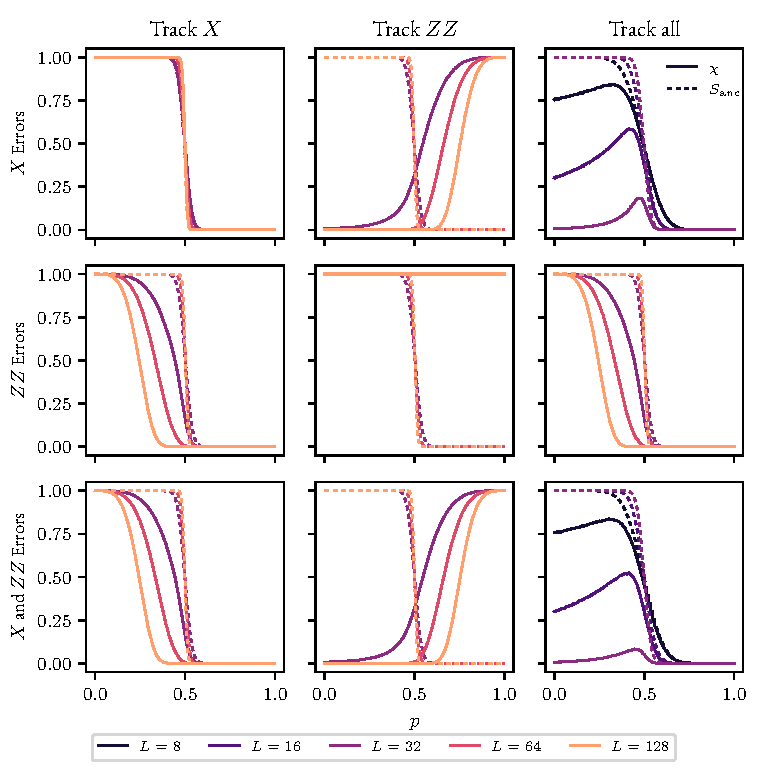
\includegraphics{errors-vs-tracked.pdf}
  \caption{Which measurement outcomes have been tracked and used to compute the
  linear cross entropy, vs the type of errors simulated.}
  \label{fig:err-vs-tra}
\end{figure}
It didn't seem to do so, so i passed \texttt{[h!]}

\begin{figure}[h]
  \centering
  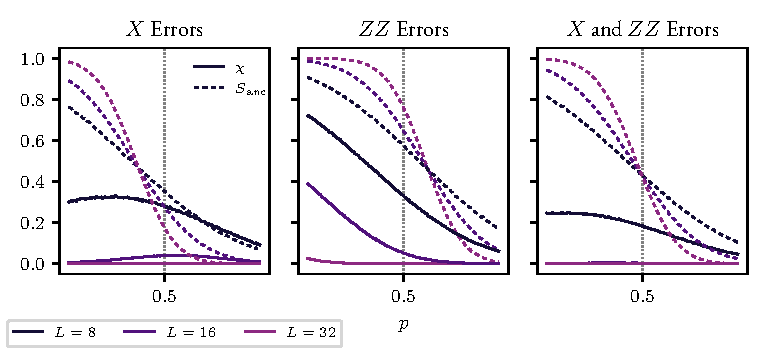
\includegraphics{anc_vs_lxe.pdf}
  \caption{Ancilla entanglement entropy and linear cross entropy for an error
  rate of $q=0.1$ to highlight the behavior of $S_\mathrm{anc}$. The system sizes are chosen smaller compared to
\cref{fig:err-vs-tra} since $\chi$ would be $0$ for larger systems. Note that
this is shown for the region around the critical point $p=.5$ in the ideal
case. This was done to make the shift of $S_\mathrm{anc}$ in $p$ more
noticeable without having the cross entropy be $0$ for ridiculously small
system sizes. Grey vertical dots indicate the critical point in the ideal case
of no errors.}
  \label{fig:large-q-anc-vs-lxe}
\end{figure}


\chapter{Upper Bound}
\label{ch:rel-ent}
\epigraph{To Infinity And Beyond}{Buzz Lightyear}

%\textcolor{red}{denk nochmal \"uber die struktur hier nach, also mit den
%numerischen approaches. naive approach zu den anderen? Auch auf simulations
%chapter verweisen!}
%
In this chapter we explore the approach of
\citeauthor{garrattProbingPostmeasurementEntanglement2023} presented in
\cite{garrattProbingPostmeasurementEntanglement2023}\footnote{While this
  reference points to a preprint on arXiv, we remark that the cited work has
since been published in
\citefield{garrattProbingPostmeasurementEntanglement2024}{journaltitle} with no
significant alterations (see Ref.
\cite{garrattProbingPostmeasurementEntanglement2024})}. They introduce a method
to probe the critical point of the phase transition of a hybrid circuit. In
particular, they make use of Klein's inequality, bounding the entanglement
entropy from above. In the present chapter we introduce the idea behind this
approach, translate it to our system---the projective transverse-field Ising
model (PTIM)---, and evaluate the quality of the resulting estimate. 

The chapter is structured as follows. In \cref{sec:upperbound-idea} we state
the principles behind the idea and derive the upper bound. Moreover, we state
and prove that for Clifford circuits, i.e. in the stabilizer formalism, there
is only a limited class of cases, where the upper bound is non-trivial. In
\cref{sec:upperbound-numerics} we introduce different numerical post-processing
algorithms, trying to combat infinities appearing, when introducing an error
model akin to the one in \cref{sec:errormodel}. The results of which are shown
and discussed in \cref{sec:upperbound-results}. Finally, we provide and discuss
regularizations of divergences, weighing out utility and computational
efficiency.

%computable quantities
%In this chapter we investigate if Klein's Inequality can assist us in obtaining
%a sensible upper bound for the entanglement entropy and thus make the
%entanglement transition visible.
%
%Idea from Altman Paper:
%\citetitle{garrattProbingPostmeasurementEntanglement2023}
%\cite{garrattProbingPostmeasurementEntanglement2023}.
%In \cite{garrattProbingPostmeasurementEntanglement2023} they introduce a method
%to obtain an upper bound on the entanglement entropy via classical
%post-processing.
%
\clearpage
\section{The Idea \& Stabilizers}\label{sec:upperbound-idea}
In this section we will introduce the upper bound on entanglement entropy,
provide an information-theoretic interpretation and derive an expression for
the quantity of interest in case of stabilizer states. First however, we will
recall the definitions of some important quantities.
\subsubsection{Entropy of entanglement}
The main quantity of interest in the whole field of entanglement transitions is
the entropy of entanglement. It is a measure for how entangled one subsystem of a
bipartite state $\ket{\phi}_{AB}$ is with the other. We recall from
\cref{sec:ent-trans} that its definition can be stated as follows
\cite{fattalEntanglementStabilizerFormalism2004}.
\begin{defn}[Entanglement entropy]\label{defn:entanglement-entropy}
  Let $\ket{\phi}\in H^{\otimes N}$ be a bipartite pure state with subsystems
  $A$ and $B$. The entropy of entanglement of $\ket{\phi}$ then reads
  \begin{align}
    %&S_E : H^{\otimes N} \to [0, N/2]\nonumber\\
    S_\mathrm{E}\left(\ket{\phi}\right) \equiv - \Tr[\rho_B \log \rho_B],
  \end{align}
  where $\rho_B = \Tr_A[\dyad{\phi}]$ is the reduced density matrix of subsystem
  $B$. Conventionally, one uses the logarithm of base 2.
\end{defn}
This quantity can be efficiently computed in clifford circuits via the
stabilizer formalism. It is important to note that the density matrix of the
whole system $\rho = \dyad{\phi}$ describes a pure state. For a more universal
measure of entropy, where the entropy of entanglement is a special case, we
need to consider the more general \emph{von Neumann entropy}.
\subsubsection{Von Neumann entropy}
The von Neumann entropy lets us quantify the average information content in a mixture of
quantum states. Originally, von Neumann introduced it as an extension of the
classical Shannon entropy to quantum systems, as density matrices serve as
extension of the classical notion of (discrete) probability distributions
\cite{vonneumannMathematischeGrundlagenQuantenmechanik1968}.\footnote{Shannon
  entropy is a measure of the average information of probabilistic events.
  Since Information is defined as $I=-\log p_x$ for some event $x$ with
  probability $p_x$, we can write down an average, $S = \expval{-\log p_x}_x =
  -\sum_x p_x \log p_x$, which defines the Shannon entropy
\cite{shannonMathematicalTheoryCommunication1948}.} 
Consequently, we can write down a definition of the von Neumann entropy.
\begin{defn}[Von Neumann entropy]\label{defn:vonneumann}
  Let $\rho$ be an $N$-qubit density matrix. The von Neumann entropy of $\rho$
  is given by
  \begin{align}\label{eq:entropy-vn}
    S\left(\rho\right) \equiv \expval{-\log \rho} = -\Tr[\rho\log\rho]
  .\end{align}
\end{defn}
For diagonalizable matrices (as we expect density matrices to be) we can also
express \cref{eq:entropy-vn} as a sum over eigenvalues $\lambda_k$ of $\rho$, i.e.
\begin{align}\label{eq:entropy-vn-sum}
  S\left(\rho\right) = -\sum_k \lambda_k \log \lambda_k
,\end{align}
where $0\leq\lambda_k\leq 1$.
This can be shown by diagonalizing $\rho$ and using the fact that the matrix
logarithm of a diagonal matrix is just the logarithm of the entries.
(Note that we set $0\cdot\log 0 \equiv 0$.)

From this definition we can already derive some important properties, namely
its lower and upper bound. Firstly, $S(\rho)$ is non-negative and $0$ iff.
$\rho$ is pure. It is easy to convince oneself of that fact. For pure states we
have $\rho = \dyad{\phi}$, which has only one non-zero eigenvalue, $\lambda =
1$. Consequently, \cref{eq:entropy-vn-sum} reduces to $S(\rho) = - 1\cdot\log 1
=0$.  Next, $S(\rho)$ is maximal for the maximally mixed state. In a
$d$-dimensional Hilbert space, the density matrix of the maximally mixed state
is $\rho = \mathds{1}/d$. Hence, \cref{eq:entropy-vn-sum} reduces to
\[
  -\sum_k \frac{1}{d} \log \frac{1}{d} = -\log \frac{1}{d} = \log d
.\]
%One property we want to emphasize in particular is that $S(\rho)$ is bounded
%from above and below; it is $0$ for a pure state and $\log d$ for a maximally
%mixed state in a $d$-dimensional Hilbert space.
\subsubsection{Quantum relative entropy}
Lastly, we want to introduce the quantum relative entropy. 
%In classical
%information theory the relative entropy of one probability distribution $p_x$
%to another distribution $q_x$ provides a measure of excess information.
%Lost in the sense that if one assumes $q_x$ as the probability distribution
%over some sample space, where 
The same way we
motivated the von Neumann entropy, we want to define a quantum mechanical
analogue to the classical relative entropy. This quantity will play a role of
major importance in this chapter and is defined as follows.

\begin{defn}[Quantum relative and cross entropy]\label{defn:rel-ent}
  Let $\rho$ and $\sigma$ be density matrices with identical dimension. The
  relative entropy of $\rho$ to $\sigma$ is
  %$S: H^{\otimes N} \times H^{\otimes N} \to \mathbb{R}^+_0 \cup \{\infty\}$
  \begin{align}\label{eq:rel-ent-defn}
    S\left(\rho\mid\mid\sigma\right) \equiv \Tr[\rho\log\rho] -
    \Tr[\rho\log\sigma] = -S(\rho) - \Tr[\rho\log\sigma]
  ,\end{align}
  with the von Neumann entropy $S(\rho)$.
  The last term in \cref{eq:rel-ent-defn}, that is, 
  \begin{align}
    S\left( \rho\mid\mid\sigma \right) + S(\rho) \equiv S_C(\rho\mid\mid\sigma) = -\Tr[\rho\log\sigma]
  \end{align}
  is known as \emph{cross entropy}. 
\end{defn}

Relative entropy, classical or quantum, quantifies excess surprisal when
one assumes $\sigma$ as a state\footnote{or probability distribution in the
classical case}, when the actual state is $\rho$. In that sense it tells us how
different two quantum states are. Interpreting it in this way also provides us
with a neat heuristic approach to possible values: the only way we do not lose
information is if we assume correctly, and in any other case we lose some. The
most extreme form of this is if $\mathrm{supp}(\rho)\cap\mathrm{ker}(\sigma)={0}$, where the
relative entropy diverges. In most general terms the relative entropy fulfils
\begin{align}\label{eq:inf-cond}
  S(\rho\mid\mid\sigma) < \infty \Longleftrightarrow \mathrm{supp}(\rho) \subseteq
  \mathrm{supp}(\sigma)
,\end{align}
where supp$(\bullet)\equiv\ $ker$(\bullet)^\perp$ is the support of a linear
operator, which is defined as the orthogonal complement to the kernel.
Alternatively, for diagonalizable matrices, it is the subspace spanned by
eigenvectors with non-zero eigenvalues
\cite{leditzkyRelativeEntropiesTheir2016,schumacherRelativeEntropyQuantum2000}.
This condition can be interpreted in a physical way. Let
\[
  \rho = \sum_i \lambda_i \dyad{\lambda_i} \quad{\text{and}} \quad
  \sigma = \sum_i \mu_i \dyad{\mu_i}
\]
be orthonormal eigendecompositions of $\rho$ and $\sigma$.
Then $S(\rho\mid\mid\sigma)$ diverges iff. there are states that $\rho$
features in its mixture that $\sigma$ does not. That is, $\rho$ has to be more
mixed than, or at least as mixed as, $\sigma$. If it is as mixed as
$\sigma$, it has to be a mixture of the same states. This means that the
information lost under the assumption of a purer state is infinite.
Since we know the von Neumann entropy to be bounded, this divergence occurs
solely in the $-\Tr[\rho\log\sigma]$ term. 

One property hinted at earlier is the non-negativity of the relative entropy.
This property goes by many different names, depending on context. For instance,
in classical statistical mechanics, this result is known as the \emph{Gibbs
inequality}. Its quantum mechanical analog is also known as \emph{Klein's
inequality}.
\subsection{Klein's inequality}
In this section we will state and prove the relation central to this chapter.
Its statement reads as follows.
\begin{thm}[Klein's inequality]\label{thm:kleins-ineq}
  The quantum relative entropy is non-negative, $S(\rho\mid\mid\sigma)\geq 0$, with equality iff.
  $\rho=\sigma$.
\end{thm}
While the statement in itself is written out rather simply, proving
\cref{thm:kleins-ineq} requires
us to introduce two auxilliary relations, namely \emph{Jensen's inequality} and
the \emph{log sum inequality}.
%Before we can go about proving \cref{thm:kleins-ineq}, we first need to
%introduce two auxilliary statements, which will be proven in the following.
%non-negativity of the classical relative entropy first. To this end, we introduce and
%prove some auxilliary lemmata, beginning with Jensen's inequality.
\begin{thm}[Jensen's inequality]\label{thm:jensen}
  Let $f$ be a convex function, that is, $f\left(\lambda x_1 + \left(
  1-\lambda \right)x_2\right) \leq \lambda f\left( x_1 \right) + \left(
  1-\lambda \right) f(x_2)$ with $0\leq\lambda\leq1$, and $X$ a discrete random
  variable. Then
  \begin{align}
    \mathbb{E}\left[f(X)\right] \geq f\left( \mathbb{E}\left[X\right] \right)
  .\end{align}
\end{thm}
\begin{proof}[Proof of Jensen's inequality]
  We will prove Jensen's inequality by induction over the mass of $X$.
  Associated with each event $x_i \in X$ is its probability $p_i$, such that
  our induction hypothesis is
  \begin{align}\label{eq:ind-hyp}
    \sum_{i=1}^n p_i f\left(x_i\right) \geq f\left(\sum_{i=1}^n p_i x_i
    \right).
  \end{align}
  As base case we have $n=2$;
  \begin{alignat*}{2}
    \mathbb{E}\left[f(X)\right] 
      &= p_1 f(x_1) + p_2 f(x_2) \\
      &= p_1 f(x_1) + (1-p_1) f(x_2) &&\qquad{\text{(Kolmogorov)}}\\
      &\geq f(p_1x_1 + (1-p_1)x_2) &&\qquad{(f\text{ convex})}\\
      &= f(\mathbb{E}[X])
  .\end{alignat*}
  For the induction step, assume \cref{eq:ind-hyp} holds for some
  $n\in\mathbb{N}_{>1}$, it must then also hold for $n+1$;
  \begin{alignat*}{2}
    \sum_{i=1}^{n+1} p_i f(x_i) 
      &= p_{n+1} f(x_{n+1}) + \sum_{i=1}^n p_i f(x_i)\\
      &= p_{n+1} f(x_{n+1}) + (1-p_{n+1})\sum_{i=1}^n \frac{p_i}{1-p_{n+1}} f(x_i)\\
      &\geq p_{n+1} f(x_{n+1}) + (1-p_{n+1})f\left(\sum_{i=1}^n
  \frac{p_i}{1-p_{n+1}} x_i\right) &&\qquad{\text{(Induction hypothesis)}}\\
      &\geq f\left(p_{n+1}x_{n+1} + (1-p_{n+1})\sum_{i=1}^n \frac{p_i}{1-p_{n+1}} x_i\right)
      &&\qquad{(f\text{ convex})}\\
      &=f\left(\sum_{i=1}^{n+1}p_i x_i\right).
  \end{alignat*}
  Since the base case and the induction step hold, we conclude that it holds
  $\forall n \in \mathbb{N}_{>1}$.
\end{proof}
\begin{cor}[Log sum inequality]\label{cor:logsum}
  Let $a_1, \ldots, a_n, b_1, \ldots, b_n \geq 0$ and let $a = \sum_i a_i$ and
  $b = \sum_i b_i$. Then
  \begin{align}\label{eq:logsum}
    \sum_{i=1}^n a_i \log \frac{a_i}{b_i} \geq a \log \frac{a}{b}
  .\end{align}
\end{cor}
\begin{proof}
  Let $f(x)=x\log x$. It is easy to convince oneself that $f$ is convex, and
  that it lets us rewrite the left side of \cref{eq:logsum}. We then have
  \begin{alignat*}{2}
    \sum_i a_i \log \frac{a_i}{b_i}
      &=\sum_i b_i f\left( \frac{a_i}{b_i} \right) 
      =b\sum_i \frac{b_i}{b} f\left( \frac{a_i}{b_i} \right) \\
      &\geq b\cdot f\left( \sum_i \frac{b_i}{b}\frac{a_i}{b_i} \right)
      &&\qquad{\text{(\cref{thm:jensen})}}\\
      &= b\cdot f\left( \frac{1}{b}\sum_i a_i \right)
      = b\cdot f\left( \frac{a}{b}\right) \\
      &= a \log \frac{a}{b}
  .\end{alignat*}
%  We can apply Jensen's inequality, since $\sum_i \frac{b_i}{b} = 1$ can be
%  taken as an average.   
\end{proof}
%Before we state the proof of \cref{thm:kleins-ineq} 
We now have all the tools ready to prove \cref{thm:kleins-ineq}. Our proof
follows the one laid out in \cite{nielsenQuantumComputationQuantum2010}, with
slight modifications.
\begin{proof}[Proof of \cref{thm:kleins-ineq}]
  Let $\rho=\sum_i p_i \dyad{i}$ and $\sigma=\sum_j q_j \dyad{j}$ be
  orthonormal decompositions for $\rho$ and $\sigma$. From \cref{defn:rel-ent}
  we can write
  \begin{align}\label{eq:ke-proof1}
    S(\rho\mid\mid\sigma) = \sum_i p_i \log p_i - \sum_i \bra{i} \rho
    \log\sigma \ket{i}
  .\end{align}
  With the eigendecomposition of $\rho$ and $\sigma$ we can write $\bra{i} \rho = p_i
  \bra{i}$ and
  \begin{align}\label{eq:ke-proof2}
    \expval{\log\sigma}{i} = \expval{\left(\sum_j \log q_j \dyad{j}
    \right)}{i} = \sum_j P_{ij}\log q_j  
  ,\end{align}
  with $P_{ij} = \ip{i}{j}\ip{j}{i} \geq 0$. 
  Plugging this into \cref{eq:ke-proof1} yields
  \begin{align}\label{eq:ke-proof3}
    S(\rho\mid\mid\sigma) = \sum_i p_i \left(\log p_i - \sum_j P_{ij} \log q_j \right)
  .\end{align}
  Note that $P_{ij}$ satisfies $\sum_i P_{ij} = \sum_j P_{ij} = 1$. We can thus
  interpret the last term in \cref{eq:ke-proof3} as an average of $-\log q_j$.
  Since $-\log$ is a strictly convex function it follows from \cref{thm:jensen}
  that
  \begin{align}
    -\sum_j P_{ij} \log q_j \geq - \log r_i
  ,\end{align}
  where $r_i = \sum_j P_{ij} q_j$, with equality iff. there exists a value of
  $j$ where $P_{ij}=1$. This implies 
  \begin{align}
    S(\rho\mid\mid\sigma) \geq \sum_i p_i \log\frac{p_i}{r_i}
  ,\end{align}
  where the equality occurs iff. there exists a $j$ with $P_{ij}=1$, i.e. iff.
  $P_{ij}$ is a permutation matrix.

  By \cref{cor:logsum} and the double stochasticity of $P_{ij}$ we obtain the
  final result
  \begin{align}
     S(\rho\mid\mid\sigma) \geq \sum_i p_i \log\frac{p_i}{r_i} \geq 1\cdot \log
     \frac{1}{1} = 0
  .\end{align}
\end{proof}

This result is essentially already our upper bound on the entanglement entropy,
since we have
\begin{align}
  \label{eq:kleins-ineq}
  S(\rho \mid\mid \sigma) \geq 0 \Leftrightarrow -\Tr[\rho\log\sigma]\geq
  S\left( \rho \right) 
\end{align}
with the relative and von Neumann entropy $S(\rho\mid\mid\sigma)$ and
$S(\rho)$ respectively. Since the von Neumann entropy is a more general form of
the entanglement entropy, we can employ Klein's inequality to upper bound the
entanglement entropy as well and thus try to find a signature of the phase
transition.

This idea was used in \cite{garrattProbingPostmeasurementEntanglement2023} for
a hybrid circuit of Haar-random 2-qubit unitaries and local $Z$ measurements.
As discussed in \cref{sec:randomcircuits}, simulating such a system is
computationally expensive.
Thus, to test their approach they
employed matrix product state (MPS) simulations. These
allow for a broader spectrum of mixed states than stabilizers do, and it is
computationally expensive, but feasible, to diagonalize the density matrix and
take its logarithm, to then compute the cross entropy upper bound. In our case,
however, we investigate a random circuit consisting of Pauli measurements only
and thus employ stabilizer simulations to run simulations on a
classical computer. As elaborated in \cref{sec:stabilizercircuits,sec:tableau},
the stabilizer formalism allows for lots of elegant computational shortcuts,
allowing efficient quantum simulations on classical computers. Consequently,
one might ask if there also is an efficient way to compute the cross or
relative entropy. We will explore this question in the next section.

%Among other things, they make use of shadow tomography to circumvent the
%post-selection problem. 
%However, they do MPS simulations, and not stabilizer. This, of course, calls
%for an adaptation (oh well\ldots).
%\begin{itemize}
%  \item \cite{garrattProbingPostmeasurementEntanglement2024} do mps
%    simulations, which, as it turns out, have a broader spectrum of mixed states than stabilizer
%    states. 
%  \item thats why they need shadow tomography and stuff
%  \item also, they do a hybrid circuit with random haar unitaries
%  \item only one type of measurement and the probability refers to if any
%    measurement is performed (on the computational basis)
%  \item MPS has lower dimensions, it is computationally expensive, but
%    feasible, to diagonalize the density matrix and take its log
%  \item[$\to$] what about clifford circuits? is there a way to write out the
%    relative entropy for stabilizers? In fact, there is:
%\end{itemize}


\subsection{Stabilizers}\label{sec:rel-ent-stab}
When resarching the quantum relative entropy and cross entropy and possible
expressions thereof in the stabilizer formalism, we have not been successful in
finding an efficient method, such as the one for the entanglement entropy
(see Ref. \cite{fattalEntanglementStabilizerFormalism2004})
\cite{veitchResourceTheoryStabilizer2014,niekampEntropicUncertaintyRelations2012,leoneStabilizerEntropiesAre2024,leonePhaseTransitionStabilizer2024,wuEntanglementUpperBound2011,vedralEntanglementMeasuresPurification1998,lindenQuantumEntropyCone2013,buExtremalityStabilizerStates2024,arabLectureNotesQuantum2024,nielsenQuantumComputationQuantum2010}.
In this section we will therefore examine the upper bound on the entanglement entropy
given by \cref{thm:kleins-ineq} in the context of stabilizers and the
stabilizer formalism. In particular, we will explore the condition of infinite
relative entropy,
provide and prove a necessary and sufficient condition
for $S(\rho\mid\mid\sigma)<\infty$ when $\rho$ and $\sigma$ are stabilizer
density matrices (\cref{prop:subgroup}), and derive an expression for finite cross
and relative entropy.

Recall that we have $S(\rho\mid\mid\sigma)<\infty$ for
supp$(\rho)\subseteq$ supp$(\sigma)$. For the proof of \cref{prop:subgroup} it
will prove useful to introduce an auxilliary lemma, which relates the support
of a density matrix to the stabilized subspace.
\begin{lem}\label{lem:supp-is-vs}
  Let $\rho$ be an $N$-qubit stabilizer density matrix with stabilizer group
  $\mathcal{S} = \langle
  g_1, \ldots, g_n \rangle$, and $0\leq n \leq N$.
  Then \[ \mathrm{supp}(\rho) = V_\mathcal{S}.\]
\end{lem}
\begin{proof}[Proof of \cref{lem:supp-is-vs}]
  By definition (see \cref{defn:stab-statespace}), we take $V_\mathcal{S}$ to be the vector space
  stabilized by $\mathcal{S}$.  Further, it is the intersection of subspaces fixed by
  each operator in $\mathcal{S}$, i.e. the eigenvalue one eigenspaces of
  elements of $\mathcal{S}$
  (see \cref{sec:stabilizergroup}). More
  formally we can write
  \[ 
    V_{\mathcal{S}} = \bigcap_{g \in \mathcal{S}}  \left\{\ket{\psi} \mid g\ket{\psi} =
    \ket{\psi}\right\} = \left\{\ket{\psi} \mid g\ket{\psi} =
  \ket{\psi} \forall g \in \mathcal{S}\right\}.
  \]
  This subspace is projected onto by
  \[ \mathbb{P}_{\mathcal{S}} \equiv \frac{1}{2^n} \prod_{g\in \mathcal{S}} \left(\mathds{1} + g\right).\]
  Recall from \cref{sec:stab-basics,defn:stab-dmat} that $\rho$ can be written as a product of
  projectors
  \[ \rho = \frac{1}{2^N} \prod_{g \in \mathcal{S}} \left(\mathds{1} + g\right)
  = 2^{n-N} \mathbb{P}_\mathcal{S} \]
  We thus have
  \[ \mathrm{supp}(\rho) = \mathrm{supp}(\mathbb{P}_{\mathcal{S}}) =
  V_{\mathcal{S}}. \]
\end{proof}

\begin{thm}\label{prop:subgroup}
  Let $\rho$ and $\sigma$ be $N$-qubit stabilizer density matrices with
  respective stabilizer groups $\mathcal{S}_\rho$ and $\mathcal{S}_\sigma$. Then
  \[ \mathrm{supp}(\rho)\subseteq \mathrm{supp}(\sigma) \Longleftrightarrow
  \mathcal{S}_\sigma \leq \mathcal{S}_\rho. \]
  That is, with \cref{eq:inf-cond}, $S(\rho\mid\mid\sigma)$ takes on finite
  values iff. $\mathcal{S}_\sigma$ is a
  subgroup of $\mathcal{S}_\rho$.
\end{thm}

\begin{proof}[Proof of \cref{prop:subgroup}]
  We will prove implication from both directions to prove equivalence.

  \enquote{$\Leftarrow$} Let $\mathcal{S}_\sigma \leq \mathcal{S}_\rho$. Then
  \begin{alignat*}{2}
    \mathrm{supp}(\rho) = V_{\mathcal{S},\rho} &= \bigcap_{g\in \mathcal{S}_\rho} \left\{ \ket{\psi} \mid
    g\ket{\psi} = \ket{\psi} \right\} \\
        &= \underbrace{\bigcap_{g\in \mathcal{S}_\sigma}
        \left\{\ket{\psi} \mid g \ket{\psi} =
        \ket{\psi}\right\}}_{V_{\mathcal{S},\sigma}}\ \ \ \cap \bigcap_{g \in \mathcal{S}_\rho \setminus
        \mathcal{S}_\sigma} \left\{\ket{\psi} \mid g \ket{\psi} =
    \ket{\psi}\right\} &&\quad{(\mathcal{S}_\sigma \leq \mathcal{S}_\rho)}\\
        &= V_{\mathcal{S},\sigma} \cap \bigcap_{g \in \mathcal{S}_\rho \setminus
        \mathcal{S}_\sigma} \left\{\ket{\psi} \mid g \ket{\psi} =
        \ket{\psi}\right\}\\
        &\subseteq V_{\mathcal{S},\sigma} = \mathrm{supp}(\sigma)
  \end{alignat*}
  which finishes the proof of this direction.

  \enquote{$\Rightarrow$} Let $V_{S,\rho} = \mathrm{supp}(\rho) \subseteq
  \mathrm{supp}(\sigma) = V_{S,\sigma}$. 
  For the proof of this direction, consider the relations between the subspaces
  of the $N$-qubit Hilbert space $H^{\otimes N}\equiv\mathcal{H}$ outlined in the following
  diagram.
  \begin{figure}[H]
    \centering
  \begin{tikzpicture}
  \matrix (m) [matrix of math nodes,row sep=3em,column sep=4em,minimum width=2em]
  {
    \mathcal{H} & V_\rho \\
     V_\sigma &  \\};
  \path[-stealth]
    (m-1-1) edge node [left] {$\mathbb{P}_\sigma$} (m-2-1)
    edge node [above] {$\mathbb{P}_\rho$} (m-1-2)
    (m-2-1) edge node [below] {$\mathbb{P}_\rho$} (m-1-2);
  \end{tikzpicture}
\end{figure}

  We can read the diagram as follows: From the $N$-qubit Hilbert space we can
  project onto the vector space stabilized by $\mathcal{S}_\sigma$, $V_\sigma$, by means of a
  projection operator. Likewise we can do the same for $V_\rho$. Since we
  require $V_{S,\rho} \subseteq V_{S,\sigma}$, the same projection that takes
  us from $H^{\otimes N}$ to $V_{S,\rho}$ will take us from $V_{S,\sigma}$ to
  $V_{S,\rho}$. It follows that $\mathbb{P}_\sigma \mathbb{P}_\rho = \mathbb{P}_\rho$.

  Let $\ket{\psi} \in V_\rho$. We thus have
  \[
    \ket{\psi} = \mathbb{P}_\rho \ket{\psi} = \mathbb{P}_\sigma \mathbb{P}_\rho
    \ket{\psi} = \mathbb{P}_\sigma
    \ket{\psi}.
  \]
  Since $\ket{\psi}$ was an arbitrary element from $V_{S,\rho}$ and $\mathbb{P}_\sigma =
  \frac{1}{2^n} \prod_{i=1}^n \left(\mathds{1} + h_i\right)$ with $h_i \in
  \mathcal{S}_\sigma$ it follows that all stabilizers of $\sigma$ also stabilize $\rho$
  and thus
  \[
    \mathcal{S}_\sigma \leq \mathcal{S}_\rho.
  \]
%  $\ket{\psi} \in V_{S,\rho}$ and $\ket{\phi} \in
%  V_{S,\sigma} \setminus
%  V_{S,\rho}$. \"o Since the stabilizer group is the
%  symmetry group of $V_S$, we can rewrite $S_\sigma$ as
%  \[ 
%    S_\sigma = \left\{ g \in G_N \mid g \ket{\psi} = \ket{\psi} \wedge g\ket{\phi} =
%  \ket{\phi} \right\},
%  \]
%  (where $G_N$ is the $N$-qubit Pauli group) 
%  as we want $S_\sigma$ to stabilize both $V_{S,\sigma}$ and its subset
%  $V_{S,\rho}$. We can then split up the condition into the intersection of two
%  sets, i.e.
%  \begin{align*}
%    S_\sigma &= \left\{ g \in G_N \mid g \ket{\psi} = \ket{\psi} \wedge g\ket{\phi} =
%  \ket{\phi} \right\}\\
%             &= \underbrace{\left\{ g \in G_N \mid g\ket{\psi}= \ket{\psi}
%             \right\}}_{S_\rho} \cap \left\{ g \in G_N \mid g\ket{\phi} = \ket{\phi} \right\} \\
%             &= S_\rho \cap \left\{ g \in G_N \mid g\ket{\phi} = \ket{\phi} \right\} \\
%               &\leq S_\rho 
%  .\end{align*}
  This concludes the proof.
\end{proof}
We have thus shown that the condition for finite values of the relative
entropy is equivalent to a simple statement about the group structure of the
respective stabilizer groups. Furthermore, we know from 
\cite{fattalEntanglementStabilizerFormalism2004} that the entropy of
entanglement can be expressed in a simple way through group properties.
We'd like for this to also be the case for other entropic quantities,
especially the cross and relative entropy, which are our main concern.

It turns out that one can indeed derive expressions for the cross and relative
entropy that put these information-theoretic quantities in a relation with
abstract group properties. Confer with
\cref{thm:cross-ent-stab,col:rel-ent-stab} for the precise statements. The
resulting expressions are remarkable in their simplicity, as well as their
similarity to each other and to previous results. As a warm-up for the proofs
of \cref{thm:cross-ent-stab,col:rel-ent-stab} we will derive an expression for
the von Neumann entropy in the stabilizer formalism first. This will also aid
in the derivation of the expression for relative entropy, since it is a
difference of the cross and von Neumann entropy.

\begin{lem}[Von Neumann entropy -- stabilizers]\label{lem:vn-ent-stab}
  Let $\rho$ be an $N$-qubit stabilizer density matrix with stabilizer group
  $\mathcal{S}_\rho$ and rank $\abs{\mathcal{S}_\rho} \equiv r$. Then
  \begin{align}
    S\left( \rho \right) = N - r
  .\end{align}
\end{lem}
\begin{proof}
  Let $\mathcal{S}_\rho$ be an $N$-qubit stabilizer group of rank $r$ with
  corresponding density matrix $\rho$.

  By \cref{defn:vonneumann}, or \cref{eq:entropy-vn-sum} in particular, we have
  \begin{align}\label{eq:entropy-vn-sum-proof}
    S\left( \rho \right) = -\Tr[\rho\log\rho] = -\sum_k \lambda_k \log
    \lambda_k
  .\end{align}
  Thus, we need to diagonalize, i.e. find the eigenvalues $\lambda_k$ of
  $\rho$.

  Since $\rho$ is a stabilizer density matrix, it can -- up to a constant
  multiple -- also be written as a
  product of projectors onto the $+1$ eigenspaces of group generators
  \begin{align}
    \rho = \frac{1}{2^N} \prod_{i=1}^r (\mathds{1} + g_i) = 2^{r-N} \mathbb{P}_\rho
  .\end{align}
  Knowing that projections are diagonalizable with eigenvalues of either $0$ or
  $1$, we know that the diagonal form of $\rho$ is the diagonal form of
  $\mathbb{P}_\rho$ with a constant multiple $2^{r-N}$, that is\footnote{Note that
    the bottom right entry need not be zero. This specific choice was made for
  illustratory purposes.}
  \begin{align}
    D_\rho = 2^{r-N} \mqty(\dmat{1,\ddots,0})
  .\end{align}
  With $\Tr[\rho] = 1$ it follows that the eigenvalues of $\rho$ must be
  $\lambda_k = 2^{r-N}$ for $k =1,\ldots,2^{N-r}$ and
  $\lambda_k = 0$ for all other $k$.
  Inserting this back into \cref{eq:entropy-vn-sum-proof} yields
  \begin{align*}
    S\left( \rho \right) 
      &= -\sum_{k=1}^{2^N} \lambda_k \log \lambda_k 
      = -\sum_{k=1}^{2^{N-r}} 2^{r-N} \log 2^{r-N} 
      = -2^{N-r} 2^{r-N} \log 2^{r-N} 
      = -\log 2^{r-N} \\
      &= N-r
  .\end{align*}
\end{proof}
The expression of the von Neumann entropy is not only interesting going
forward, e.g. in the derivation of the relative entropy, but also from a group
theoretic perspective. That is, it should be noted that by asking an
information-theoretic question, we got a group theoretic answer. Let us
convince ourselves that it is a reasonable one, by testing it on our intuition
on entropy.

With $N$ qubits we have a generating set of size $N$, at most. In the case
where we have $N$ generators, the state associated with the stabilizer group is
a pure state, and the entropy should be $0$, which is the case for $r=N$. For
the maximally mixed state, the generating set is the empty set and the
stabilizer group the trivial group. In accordance to our expectations, this
should yield $\log(2^N)= N$ for the von Neumann entropy. Indeed, since the size of
the empty set is $0$, we have that $r=0$ and thus $S(\rho) = N$.

Removing one generator thus increases entropy by $1$, or put differently,
starting from the empty set and adding generators to it decreases entropy by
$1$ for each generator added. This too should come to no surprise, as we know
that for each generator removed (added) from a full set of stabilizers, we
double (halve) the stabilized state space, effectively creating (purifying) a
perfect mixture of stabilized states.

\begin{thm}[Cross entropy -- stabilizers]\label{thm:cross-ent-stab}
  Let $\rho$ and $\sigma$ be $N$-qubit stabilizer density matrices with
  respective stabilizer groups $\mathcal{S}_\rho$ and $\mathcal{S}_\sigma$ that
  satisfy $\mathcal{S}_\sigma \leq
  \mathcal{S}_\rho$. Further, let $\abs{\mathcal{S}_\sigma} \equiv s$. Then
  \begin{align}\label{eq:cross-ent-stab}
    S_C(\rho\mid\mid\sigma) = N - s
  .\end{align}
\end{thm}

\begin{proof}
   Let $\mathcal{S}_\rho$ and $\mathcal{S}_\sigma$ be $N$-qubit stabilizer
   groups that satisfy $\mathcal{S}_\sigma \leq \mathcal{S}_\rho$. Their
   respective density matrices can be written as
   \begin{align}
     \rho = \frac{1}{2^N} \prod_{i=1}^r (\mathds{1} + g_i) \quad{\text{and}}
       \quad \sigma = \frac{1}{2^N} \prod_{i=1}^s (\mathds{1} + h_i)
   \end{align}
   with $r \equiv \abs{\mathcal{S}_\rho}$ and $s \equiv
   \abs{\mathcal{S}_\sigma}$. Since we require $\mathcal{S}_\sigma \leq
   \mathcal{S}_\rho$, we can construct a generating set $G_\sigma$ of
   $S_\sigma$, where each element of $G_\sigma$ commutes with the generating
   set of $G_\rho$. Note that the generating sets are not necessarily
   identical. However, since $\mathcal{S}_\sigma$ is by construction a subgroup
   of $\mathcal{S}_\rho$, which in turn is an abelian subgroup of
   $\mathcal{P}_N$, all elements of $\mathcal{S}_\sigma$ commute with all elements of
   $\mathcal{S}_\rho$. It follows that the density matrices themselves also
   commute, i.e.
   \begin{align}
      \left[\rho, \sigma\right] = 0
   .\end{align}
   It is a well-known fact from linear algebra and functional analysis that
   commuting operators share a common eigenbasis and can be diagonalized
   simultaneously. We therefore write $\rho = UD_\rho U^{-1}$ and $\sigma =
   UD_\sigma U^{-1}$ with transformation matrix $U$ and corresponding diagonal
   matrix $D_{\rho / \sigma}$. We also have that the logarithm of a diagonalizable
   matrix is \cite{hallElementaryIntroductionGroups2000}
   $$\log \sigma = U \log D_\sigma U^{-1}.$$ Consequently,
   \begin{align}
      S_C(\rho\mid\mid\sigma) = -\Tr[\rho \log\sigma] = -\Tr[U D_\rho U^{-1} U \log D_\sigma U^{-1}] =
      -\Tr[D_\rho \log D_\sigma] 
   .\end{align}
   With $D_\rho$ and $D_\sigma$ diagonal we can write the trace as
   \begin{align}\label{eq:the-sum}
      -\Tr[D_\rho \log D_\sigma] = -\sum_k \lambda_k \log \mu_k
   \end{align}
   with the eigenvalues $\lambda_k$ and $\mu_k$ of $\rho$ and $\sigma$,
   respectively.

   As we know from the previous proof, $\lambda_k = 2^{r-N}$ for
   $k=1,\ldots,2^{N-r}$ and $0$ otherwise, and analogously, $\mu_k = 2^{s-N}$
   for $k=1,\ldots,2^{N-s}$ and $0$ otherwise. Note that the subgroup condition
   implies that $r\geq s$ or more specifically $N-r \leq N-s$. This ensures that to every non-zero entry in
   $D_\rho$ there is a corresponding non-zero entry in $D_\sigma$. In other
   words, for all $k$, $\lambda_k \neq 0 \Rightarrow \mu_k \neq 0$. More
   importantly for us, however, is the contrapositive, $\mu_k = 0 \Rightarrow
   \lambda_k = 0$, which tells us that any divergence that might occur
   in the logarithm gets intercepted by a leading factor of $0$.

   Inserting this into the sum in \cref{eq:the-sum} we get
   \begin{align}
      -\sum_i 2^{r-N} \log 2^{s-N} =
      -2^{N-r}2^{r-N}\left(s-N\right)= N-s
   ,\end{align}
   which concludes the proof.
\end{proof}

Although \cref{thm:cross-ent-stab,eq:cross-ent-stab} are in dire need to be
discussed, we do not want to fail to mention that the relative entropy between
two stabilizer density matrices follows as a corollary.

\begin{cor}[Relative entropy -- stabilizers]\label{col:rel-ent-stab}
  Let $\rho$ and $\sigma$ be $N$-qubit stabilizer density matrices with
  respective stabilizer groups $\mathcal{S}_\rho$ and $\mathcal{S}_\sigma$,
  where $\abs{\mathcal{S}_\rho}
  \equiv r$ and $\abs{\mathcal{S}_\sigma} \equiv s$. If $\mathcal{S}_\sigma \leq
  \mathcal{S}_\rho$, then the relative entropy of $\rho$ to
  $\sigma$ is
  \begin{align}
    S\left(\rho\mid\mid\sigma\right) = r - s
  .\end{align}
\end{cor}

\begin{proof}
  Let $\rho$ and $\sigma$ be density matrices satisfying the stated
  requirements, $\mathcal{S}_\sigma \leq \mathcal{S}_\rho$ in particular. From \cref{defn:rel-ent},
  or more precisely \cref{eq:rel-ent-defn}, we have
  \begin{align}
    S\left( \rho\mid\mid\sigma \right) = -S\left( \rho \right)
    -\Tr[\rho\log\sigma]
  .\end{align}
  Inserting our results from \cref{lem:vn-ent-stab,thm:cross-ent-stab} yields
  \begin{align}
    -S\left( \rho \right) -\Tr[\rho\log\sigma] = -(N-r) + N - s = r - s
  .\end{align}
\end{proof}

%What are the information-theoretic implications of \cref{thm:cross-ent-stab}?
Notice that although it is defined as a quantity relating $\rho$ to $\sigma$,
there is no explicit dependence of $\rho$ in \cref{eq:cross-ent-stab}.
What \cref{thm:cross-ent-stab} seems to imply is that the cross entropy between two stabilizer
density matrices $\rho$ and $\sigma$ just amounts to the von Neumann entropy of
$\sigma$. However, this is where one needs to be careful. While the resulting
numerical value is entirely dependent on $\sigma$ and its stabilizer group
alone, we have an implicit dependence through the requirement that
$\mathcal{S}_\sigma \leq \mathcal{S}_\rho$. Since we were able to show that the
cross entropy is infinite in the converse case (see \cref{prop:subgroup}), we
could add the $\rho$ dependence back in, i.e.
\begin{align}\label{eq:cross-ent-cases-infty}
  -\Tr[\rho\log\sigma] = \begin{cases}
    N - \abs{\mathcal{S}_\sigma} &\quad{\mathcal{S}_\sigma \leq
    \mathcal{S}_\rho}\\
      \infty &\quad{\mathcal{S}_\sigma \not\leq \mathcal{S}_\rho}
  \end{cases}
.\end{align}
This detail will be important later on, as we try to avoid explicit
dependences on $\rho$, which would take us back to the sampling problem.

The independence of $\rho$ in the first case, however, is still quite a
remarkable result. Let's examine the expression and convince ourselves that
this simplicity is no accident.
From the subgroup condition we know that the state
described by $\sigma$ needs to be more mixed or at least as mixed as $\rho$.
That is, the probability distribution on the state space represented by $\sigma$ contains
more states than $\rho$. However, all states of $\rho$ are featured in
$\sigma$ with uniform probability. Any state in the mixture of $\sigma$ thus
gets assigned the same weight when averaging. Additionally, the probabilities
over the larger state space are uniformly distributed as well, turning $\log
\mu_k$ into a constant factor. It is therefore an average of a constant over a
uniform probability distribution, which is just the constant itself. 

%
%\textcolor{red}{Something something, cross entropy independent of $\rho$,
%  essentially the von neumann entropy of $\sigma$, which is, dare I say,
%rather trivial compared to what one expects from a logarithmic quantity}

We have discussed the mathematical and information-theoretic aspect of the
derived statements, but we should also think about the physical
implications of these statements. Although we summarized the idea, we want to
reemphasize the utility behind these expressions.
Our ultimate goal is an upper bound on the half-system
entanglement entropy, $S_E\left( \rho \right)$,\footnote{Here, $\rho$ refers to
the reduced density matrix of half the system, where the entire system is in
the pure state $\ket{\phi}$} which can be derived from \cref{eq:kleins-ineq}.
With that, we try to detect a signature of the critical point of the phase
transition found by classical simulations. Recall that the half-system
entanglement entropy is non-linear in the density matrix, that is, it is an
observable of the state itself, requiring exponentially many copies of the same
state. Therefore, it is infeasible, and practically impossible, to perform
measurements quantifying entanglement with the entanglement entropy. However,
by \cref{eq:kleins-ineq} we can obtain an upper bound, $S_E\leq
-\Tr[\rho\log\sigma]$, thus circumventing the sampling problem. The choice of
$\sigma$ has some degree of arbitraryness; as long as 
$\mathrm{supp}\left( \rho \right) \subseteq \mathrm{supp}\left( \sigma \right)$ 
we get a finite upper bound, and even have equality if $\rho = \sigma$.  But
this is not the whole picture. It stands to reason that we \emph{should} be
picky with our choice of $\sigma$ and be consistent with it.  In particular, we
ideally would like to relate $\sigma$ to the experimental state
$\rho$ in some way or another. This can be done by classically reconstructing
$\rho$ by means of projecting the measurement outcomes from the record
$\mathbf{m}$. Then, by tracing out half of the system, we obtain some
$\sigma$, which we can use in the upper bound. The classical post-processing of
the measurement record requires us to efficiently simulate the system, as well
as to be able to project onto specific outcomes. 
To this end, we prefer to use
stabilizer simulations, as they allow the efficient simulation and
post-processing of our system. With \cref{thm:cross-ent-stab} we now
additionally have an efficient method of computing the upper bound to the
entanglement entropy, such that the inequality becomes
\begin{align}
  S_E \leq N-s
.\end{align}
The following sections therefore pertain to the various possible
post-processing algorithms one might make use of. 
%\subsection{Shadow Tomography}
%these papers are cited in
%\cite{garrattProbingPostmeasurementEntanglement2023} for shadow tomography:
%\begin{itemize}
%  \item \citetitle{elbenRandomizedMeasurementToolbox2022}
%    \cite{elbenRandomizedMeasurementToolbox2022}
%
%    Review paper. Context: "It will be useful to first outline shadow
%    tomography \cite{elbenRandomizedMeasurementToolbox2022} in its simplest
%    incarnation for a single qubit"
%
%    It has indeed been useful, but I gotta admit, i didn't get my outline from
%    this one, but from:
%  \item \citetitle{huangPredictingManyProperties2020}
%    \cite{huangPredictingManyProperties2020} 
%
%    In this paper, shadow tomography is the main thing investigated. Context:
%    "Generalizing \ldots to multiple qubits is straightforward
%    \cite{huangPredictingManyProperties2020}: one possibility is to construct
%    $N$-qubit shadows as the tensor products of $N$ objects with the structure
%    \ldots"
%\end{itemize}
%
%Some more shadow tomography papers:
%\begin{itemize}
%  \item \cite{aaronsonShadowTomographyQuantum2018} shadow tomography defined
%    for the first time
%  \item IDK where i want to include this one, but i think it will be
%    interesting to study a bit more:
%    \cite{tothEntanglementDetectionStabilizer2005} Entanglement witness
%\end{itemize}
%
%This one is not on shadow tomography, but is cited in
%\cite{garrattProbingPostmeasurementEntanglement2023}, which got me hella
%frustrated, since I did not know what the hell they meant with "Our discussion
%in this section largely follows Ref.
%\cite{garrattMeasurementsConspireNonlocally2023}" if it does not really match
%the vibe of \emph{this section}.
%


\section{Naive approach}\label{sec:naive-approach}
The key idea of the upper bound is to have a quantity that is linear in $\rho$.
By obtaining a measurement record $\vb{m}$, we can try and classically
reconstruct the experimental density matrix $\rho$ from the record. Since we
are doing a classical computation, we have the advantage of being able to
project onto measurement results. We therefore can -- naively -- attempt a
reconstruction of our experiment based on the data. Of course, in our case, we
also use a classical simulator to generate data.

\subsection{Methods}
After the data has been generated we do as we did before in \cref{ch:lxe} and
project the measurement outcomes onto $\sigma$. However, we start from the same
state $\rho = \sigma = \dyad{GHZ+}$. After we have completed the circuit, we
trace out one half of the qubits and compute the cross entropy, which is given
by \cref{eq:cross-ent-stab}. 

For our prospective numerical experiments, we would therefore have them support
the simulation of mixed states, since we might encouter them by means of
partially tracing out the system. To this end, we refer to \cref{ch:mixed}, in
particular \cref{sec:mixed-states,sec:sim-entropies,sec:ptrace}. In these
sections, we introduce the algorithms used to realize mixed states, the
different entropic quantities, and the partial trace, respectively. Of course,
we additionally need to adapt the projection function, since we now
\emph{force} the projection upon the state. For the computation of the linear
cross entropy, it sufficed to know if projections were successful all the way
through. If they weren't, we would simply break the loop over the measurement
record and stop the projections. Here, we really want a faithful reconstruction
of the density matrix. The algorithm to force projections is outlined in
\cref{alg:force-project}.

As we use the general setup from \cref{ch:lxe}, we also employ the error model
introduced in \cref{sec:errormodel} to emulate noise in the circuit. This is to
ensure comparability between the general approaches of the linear cross entropy
and the cross entropy as upper bound.

As we have access to the \enquote{experimental} density matrix $\rho$ through
our numerical simulation, we employ the implementation of the cross entropy as
outlined in \cref{thm:cross-ent-stab}. An important detail to note however is
that we do not want infinities appearing in our data. As such, 
in the case of $\mathcal{S}_\sigma \not\leq
\mathcal{S}_\rho$, we add $N /2$, where $N$ is the number of qubits in the
system. This amounts to replacing the density matrix $\sigma$ by the maximally
mixed state.

\subsection{Results}

In \cref{fig:naive-svn-vs-se-no-error} the results of the upper bound is shown
in the case of no noise in the circuit.
\begin{figure}[t]
  \centering
  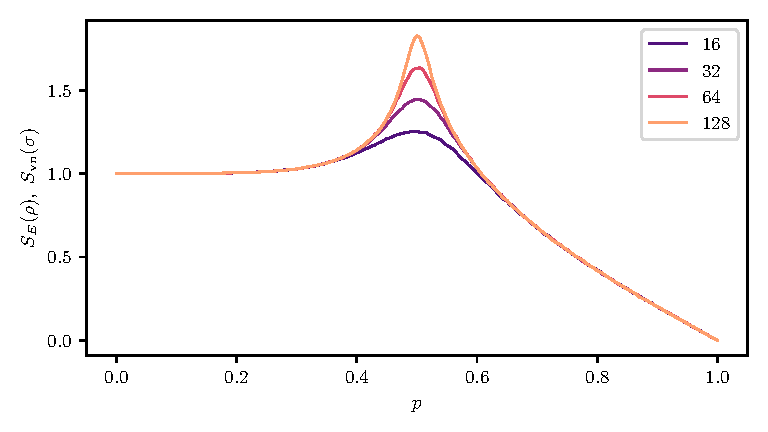
\includegraphics{naive_approach_cleansystem_soloplot.pdf}
  \caption{Cross and entanglement entropy in the noiseless system. We project
    the measurement outcomes from $\rho$ onto $\sigma$ if possible. Note that
    we here use periodic boundary conditions. Each datapoint corresponds to
    $\sim 10^5$ samples.}
  \label{fig:naive-svn-vs-se-no-error}
\end{figure}
\Cref{fig:naive-svn-vs-se-no-error} shows that there is perfect overlap between the original and
the replicated system in the noiseless case. This is also what one would
expect, since we effectively computed the entanglement entropy of a pure state that
happens to have had the same measurement record as $\rho$. And incidentally,
every outcome in the measurement record corresponded to an outcome that could
be projected perfectly onto $\sigma$. We thus perfectly saturated the upper
bound \cref{eq:kleins-ineq}. 

We now turn towards a more realistic scenario, namely that of a noisy circuit.
The error model we use to emulate noise is the one introduced in
\cref{sec:errormodel}. Note that we force the projections onto $\sigma$, and
thus should recover a close estimate of the experimental density matrix. If it
turns out that the density matrix obtained from the experiment does not have
support in $\sigma$, we replace the appearing infinity with $L /2$, where $L$
is the number of qubits.
\begin{figure}[t]
  \centering
  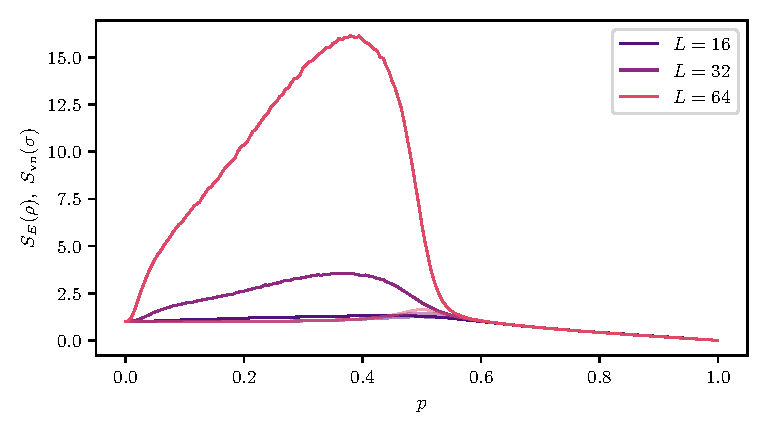
\includegraphics{naive_approach_xerrors_soloplot.pdf}
  \caption{Cross and entanglement entropy in the system with projective $X$
  errors. Measurement outcomes from a simulated experiment are projected onto a
replica in the classical simulation. If the subgroup condition is not met, we
replace the appearing infinity with $L /2$. }
  \label{fig:naive-svn-vs-se}
\end{figure}

\Cref{fig:naive-svn-vs-se} shows that the naive approach fails here already. In
the $p< p_c$ regime we often need to correct for infinities in the sample,
which get replaced, yes, but since the trivial upper bound is so far off the
actual entanglement entropy, we have this diverging behavior even for
relatively small systems, which is why only systems up to $L=64$ are shown. For
$p>p_c$ we saturate the bound again, since the $X$ noise commutes with the then
more frequently occuring $X$ measurements of the circuit, thereby restoring the
adherence to the subgroup condition.

This tells us that we need some way to cope with noise. The subgroup condition
requires us to detect the errors, since errors which are not succeeded by a
measurement (of any kind) will lead to a change in the structure of
$\mathcal{S}_\rho$, which are never detected. This undetectable change, as we
can tell from \cref{fig:naive-svn-vs-se}, happens if an error occurs on a qubit
in a state stabilized by an operator, which anticommutes with the type of
noise. For instance, if an $X$ error occurs on a qubit stabilized by $Z$. Since
$X$ measurements are more frequent for $p> 1/2$, the $X$ noise is directly
mitigated by the frequent measurements. 

What about the part where $X$ measurements aren't as frequent? We can again
estimate a probability of not detecting the altering of the stabilizers.
Imagine an error occurs in the very last layer, i.e. after all the measurements
in the circuit happened. This is the complementary probability to no errors
occuring. We thus have
\begin{align}
  P(\#\mathrm{err}>0) = 1-(1-q)^L
.\end{align}
As simple example, consider the probability of an $X$ error occuring in the
very last layer of a system with $L=32$ qubits. The probability that an error
doesn't get detected is $P\simeq\num{.275}$. Thus, about 1 in every 4 samples
would yield infinity as upper bound, which is useless. We thus make the rather
unphysical assumption that no error is allowed to happen after a certain
threshhold. As we design the circuit in a classical simulator as well, we
simply restrict the allowed errors occurring.

%\begin{itemize}
%  \item subgroup condition requires errors to be detected (and dealt with in
%    some way)
%  \item errors which are not succeeded by a measurement will lead to a change
%    in the group structure of $S_\rho$ such that $S_\sigma$ \enquote{never has
%    the chance to adapt}
%  \item maybe we should also implement some ideas from the shadow tomography
%    dings, such that errors are circumvented
%  \item Undetectable change in group structure happens if an error happens on a
%    qubit in a state stabilized by an orthogonal operator, e.g. an $X$-error if
%    the qubit is stabilized by $Z$.
%  \item The probability of any error happening in the last layer (i.e. after
%    all measurements in the circuit happenend) is $1-$ the probability of no
%    error, which is given by the binomial distribution
%    \[ P(\#\mathrm{err}>0) = 1-\binom{N}{0} (1-q)^N=1-(1-q)^N. \]
%  \item For $q=\num{0.01}$ and $N=32$ we have $P\simeq .275$
%  \item Of course, this probability says nothing about the actual simulation
%    (except for $p=0$) as it could be an error which was preceeded by an $X$
%    measurement.
%  \item That being said, you could technically compute this probability
%    analytically, by going through each layer and multiplying the probabilites
%    for \(X\) and not $ZZ$ happening to get the actual probability of failure
%   \item This is way too complicated, just to get an estimate on how many
%     simulations will end in $\infty$ for \cref{eq:kleins-ineq}. 
%\end{itemize}

%Let us now consider the information-theoretic implications of \cref{eq:cross-ent-stab}. 
Furthermore, recall that the cross entropy is a measure of the quality of an estimate of a
probability distribution \cite{coverElementsInformationTheory2006}. As we are
essentially estimating the experiment, represented by the density matrix
$\rho$, with a uniform probability distribution over the support of $\rho$, the
quality of our estimate depends only on how many events (or in this case,
states) we choose to include in our estimate. In other words, we project onto
an eigenstate $\ket{\phi}$ of $\rho$, where our estimate of the probability of
$\ket{\phi}$ is scaled by how many other states we consider with equal
probability. Alternatively, in the case where the subgroup condition is not
met, we do \emph{not} have $\ket{\phi}$ in $\mathrm{supp}\left( \sigma
\right)$. In this scenario, we project onto the $0$ vector, giving us a
divergent term in the cross entropy.
This also shows how stabilizer
states are particular in that sense. Any stabilizer density matrix we choose
for $\sigma$ will yield this result, independent of $\rho$, as long as $\rho$
is a valid density matrix. 

This means that if we were to continue with the cross entropy and the upper
bound in a pure stabilizer setting, we should think about how we could have a
finer-grained selection of values the cross entropy can take up. If we only
insert pure states, we might get lucky a couple of times, but in all
generality, we will fail to estimate the density matrix obtained in an
experiment. Thus, for the purely numerical approaches, we should abandon the
naive one in favor of reconstruction algorithms that include a broader set of
states to support $\rho$. Of course, they should, as we have been made aware by
the previous results, ensure the fulfillment of the subgroup condition as well. 

\clearpage
\section{Other numerical approaches}\label{sec:upperbound-numerics}

We have seen that the naive approach fails once noise comes into play.
Especially if the modelled errors are not succeeded by a measurement natively
included in the circuit. We have also noted that due to the limitations of the
stabilizer formalism, we either end up in agreement with the experiment or add
infinities to the mix. As we would like to stay in the stabilizer formalism,
since it allows ploynomial-time simulation of the quantum circuit in question,
we need to cope with noise in a different way, that also encompasses the tools
we have at our disposal. 

We have further found an irreconcilable limit to \cref{eq:kleins-ineq} in the
form of errors appearing in the last measurement layer. For all the further
considerations, we disallow errors after the last measurements. This is, of
course, an unphysical assumption to make, but this is, as of right now, not our
main concern, as we right now want to test the limits of \cref{eq:kleins-ineq}
on our system. This was one of them. If we relax the assumption of errors
happening everywhere, we could try other approaches and maybe get an idea of
how viable the general approach of an upper bound is to find a signature of the
entanglement transition.  With the primer of the previous protocol failing, we
also include two new quantities next to the cross entropy. 

%In the simulation we trace out half the system in both cases, and then
%determine if they are subgroups of one another
% 
%In case they are not, there are infinities to deal with.
% 
%We deal with them by effectively replacing the algorithmically obtained
%   $\sigma$ by the maximally mixed state $2^{-L /2} \mathds{1}$. That is,
%   instead of adding $\infty$ (or technically, \texttt{quiet\_nan}) to the
%   ensamble average, we add $L /2$.
% 
%Since this is once more not how a usual physical observable behaves, we
%   keep track of how often we cheat the simulation algorithm
The first one is the \enquote{infinity ratio}, i.e. the ratio of simulations
not agreeing with the subgroup condition, therefore having diverging
contributions in the sample average, which we regularize \enquote{primitively}
by replacing it with the trivial upper bound $L /2$. Since this is once more
not how a conventional physical observable behaves, we keep track of how often
we cheat in the simulation algorithm. 
This measure therefore quantifies if
the algorithm we conceived really did work as intended or if we made conceptual
errors. Furthermore, it aids in explaining the behavior of the cross entropy,
as we can then gauge if anomalously high values for the upper bound come from
the algorithm or the primitive regularization. 

To this end, we also have the next quantity, which is the von Neumann entropy
of the entire density matrix before the partial trace over half the system.
This measure quantifies the degree of mixedness left in the system at the very
last timestep. For the naive approach, this last quantity is obviously $0$
everywhere, since it produces pure states only.

The following sections introduce the methodology behind two numerical
post-processing algorithms that utilize mixed states with the aim to uphold the
subgroup condition, as well as show the results of the performed simulations.

%\begin{itemize}
%  \item Naive approach fails because of errors, which cannot be detected by
%    construction
%  \item also, because so far we have only dealt with pure states.
%  \item we thus need a new classical post-processsing algorithm
%  \item first, we need to disallow errors after the last couple of
%    measurements, since these are the ones that make it into the subgroup check
%  \item this is, of course, an unphyisical assumption to take, but thats not
%    our main concern. informally speaking, we want to test the limits of
%    \cref{eq:kleins-ineq} for our system. We found this irreconcilable one in
%    the context of our model
%  \item   \item next, we have this condition of diverging cross entropy. Why not go in
%    reverse and try an algorithm, which has the stabilizers of $\sigma$ be a
%    subgroup of $\rho$.
%  \item we can do that by modifying the projections slightly
%  \item in the following sections we explore some approaches to modify the
%    projection operation to incorporate mixedness
%\end{itemize}

\subsection{Minimal Mixing}\label{sec:minimal-mixing}

The first post-processing algorithm we introduce is what one could call
\enquote{minimal mixing}. In the following, we will introduce the algorithm and
the results. Note that the presentation of the results parallels the
presentation shown in \cref{fig:err-vs-tra}, with the methods to obtain this
it mirroring the ones in \cref{ch:lxe}. As such, we assume knowledge of how
\cref{fig:err-vs-tra} is to be read.

\subsubsection{The algorithm}

We start our classical reconstruction in the same state as the initial state of
the experiment, for us it is $\dyad{GHZ+}$ in particular. Then, we project onto
the measurement outcomes where possible. In a noiseless circuit, this recovers
the standard entanglement entropy once more. Once we introduce noise this will
no longer be given. Recall the scenario shown in \cref{fig:mech-b1-lxe}. In
this case we had that the projection was successful only with probability $1
/2$ and unsuccessful also with probability $1 /2$.

For this numerical approach, we choose to ignore the stabilizer generator with
the failed projection. That is, we replace the stabilizer by $\mathds{1}$ where
the incompatibility was detected, instead of forcing the projection. This
should, in principle uphold the subgroup condition, since we remove particular
generators from the generating set. Until it gets measured again, we have that
this stabilizer is not a generator. The technical details behind the
implementation are laid out in \cref{sec:other-dingers,alg:minimal-mixing}.

The procedure to compute the cross entropy is still the same as before. We
trace out one half of the system, then perform the subgroup check, and add
\begin{align}\label{eq:cross-ent-cases-infty}
  \tilde{S}_C(\rho\mid\mid\sigma) = \begin{cases}
    N - \abs{\mathcal{S}_\sigma} &\quad{\mathcal{S}_\sigma \leq
    \mathcal{S}_\rho}\\
      \frac{L}{2}  &\quad{\mathcal{S}_\sigma \not\leq \mathcal{S}_\rho}
  \end{cases}
\end{align}
to the sample average. In addition to the previous protocol, we also compute
the von Neumann entropy of the full state obtained by the algorithm, as well as
count how often we added $L /2$ in the case of a mismatching group structure.

One critique that could immediately be raised at this point is the (ab)use of
mixed states in this context. Each time we come across a discrepancy, we
throw out the generator in question, even though this is the most recent
information we have on the state of the system. However, we have already made
some unphysical assumptions before, and this is no exception. At this point we
want to test the performance of the upper bound in the extreme case of
stabilizers and we want to use all the tools available to us, and selectively
removing stabilizer generators from the generating set is one of them.
\emph{How} we select them is then judged by the performance of the selection in
the numerical simulation.

\subsubsection{Results}

\Cref{fig:min_mix-svn_se-4x3} shows the upper bound (opaque) and the
entanglement entropy (transparent) as a function of the probability parameter
$p$ for the minimal mixing algorithm. For the \enquote{no error, track
everything} case, we---unsurprisingly---recover the identical behavior to the
regular entanglement entropy, since every projection is successful. 

For all the marginalized runs, we can see that they end up in the infinite case
rather often (see also \cref{fig:min_mix-inftyratio-4x3}). This is because we
measure instead of project. Thus, we might measure and get a random result that
is orthogonal to the one we would have projected onto, even if there is no
error present.  In the case where we marginalized out $ZZ$, i.e. the
\enquote{Track X} column, we have that for no errors and $p=0$, the cross
entropy agrees with the entanglement entropy. This is because there are no $X$
measurements to track either way, so there is nothing that can go wrong.

However, once we have even the tiniest amount of $X$ measurements, everything
goes horribly wrong.  Even for relatively small systems of $L=16$ and $L=32$
qubits, we almost always end up at the trivial upper bound of $S_E \leq 8$ and
$S_E \leq 16$ respectively.  An interpretation in terms of quantum error
correction would be that we did not correct an error, but chose to let it happen.
In a sense, this plot tells us that we have done a poor job correcting errors,
or rather that we did not do so at all.

In the case where we only tracked the outcome of $ZZ$ measurements, this
phenomenon is not as intense as it is for the outcome of $X$ measurements. 
This can be explained with the fact that we perform stabilizer
measurements, i.e. we know where errors happened, yes, but we do not know
the outcome of them. In spirit, this is similar to a decoding or error
correcting protocol \cite{roserDecodingProjectiveTransverse2023}. Also, the
scaling of this particular plot is exponential in the system size up to the
theorized critical point, where it flattens and goes to the trivial upper
bound.

What about the noisy circuits?
Recall from the linear cross entropy that in the case of
$X$-noise occurring, i.e. projective $X$ errors,
we had that the marginalized $ZZ$ / Track $X$ plot
with $X$ errors was identical to the ideal system. This was due to the fact
that the linear cross entropy only contained the probabilities of success or
failure, and the fact that the error type commuted with the tracked measurement
outcomes. Here, we do not have this luxury. In fact, the same things that apply
to the case without errors apply here. We even notice that for $p=0$, there
is no agreement anymore, since we effectively shifted the lines to the left a
bit. Before, every $ZZ$ measurement was a genuine stabilizer measurement, since
we measured generators of the stabilizer group. This is not the case anymore,
since even with $p=0$, we have sporadic creation and annihilation of clusters
everywhere, which perturb the entanglement structure.  Sure, it should be
corrected instantly, since we perform $ZZ$ measurements everywhere at any time.
But this is not enough if errors are sufficiently frequent, which is the case
for larger systems.  This is also the reason why we chose to show all these
situations for smaller system sizes only.

When tracking only the outcomes of $ZZ$ measurements, we find that we do not
have the nice exponential growth, but a superexponential growth.  the
occurrence of $X$ measurements, which we do not even try and \enquote{guess}
the outcome is now larger.  The regime where we only have trivial upper bounds
is shifted to the left slightly.  The more interesting plot is the one where we
track everything.  We must have failed in our quest to bring everything under
the umbrella of the $\mathcal{S}_\rho$ stabilizer group, since we can see a
disturbing discrepancy between $S_E$ and the cross entropy.
  
This discrepancy can be explained by the fact that two measurement layers are
not enough to fully rule out undetectable errors. We can have clusters emerging
that fit the measurement outcomes just enough so that they bypass our
detection/error handling scheme.  However, they do not bypass the subgroup
check. With $X$-errors occurring, we, of course, correct a lot of errors, which
can be seen in the fact that we have a tighter upper bound towards $p=0$.
Closer to the critical point we find a peak, where $X$ errors are frequently
contributing to the creation of unforseen clusters, which bypass the error
handling scheme.  In the regime of $p > p_c$, we find that there is again
agreement with the entanglement entropy, since $X$ measurements are more
frequent to $ZZ$ measurements $X$ errors, such that noise is.

For $ZZ$ errors, the converse is the case, while we have a combination of both
divergences in the case where we include both types of errors.

\begin{figure}[p]
  \centering
  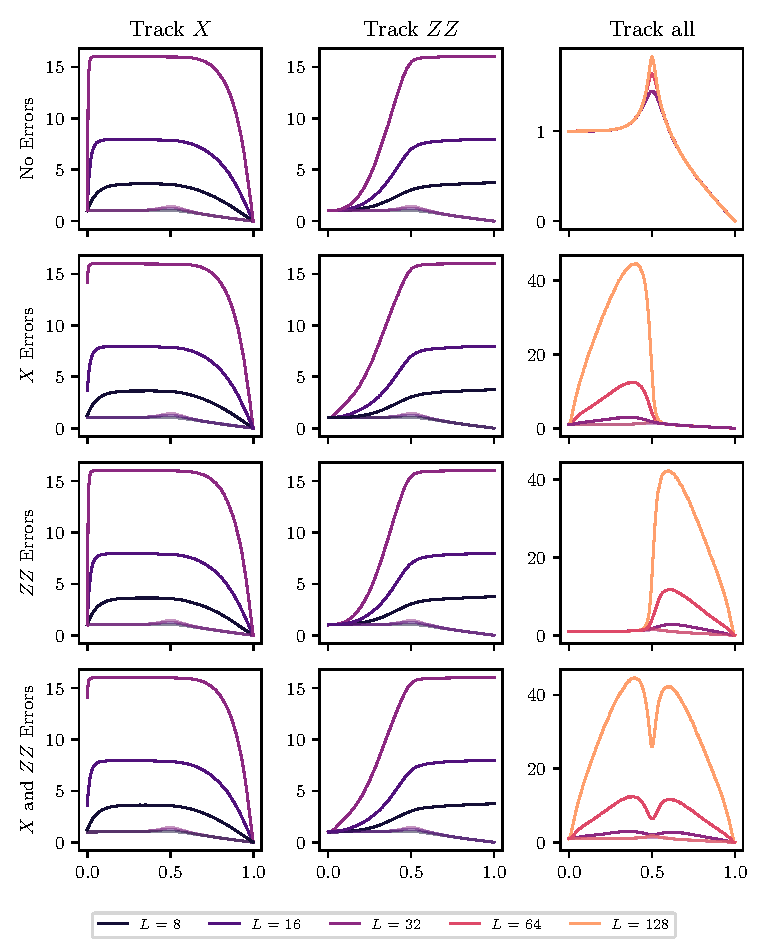
\includegraphics{minimal_mixing-4x3-svn_se.pdf}
  \caption{Cross Entropy and entanglement entropy of selected system sizes with
    periodic boundary conditions for the \enquote{minimal mixing} algorithm. 
  To be able to adequately compare it to LXE the
different trackings and errors are shown in the same manner as in
\cref{fig:err-vs-tra}.}
  \label{fig:min_mix-svn_se-4x3}
\end{figure}

We can therefore infer already that we have not done enough to sanitize the
input of the subgroup check. To confirm this suspicion, consider
\cref{fig:min_mix-inftyratio-4x3}.  In \cref{fig:min_mix-inftyratio-4x3} we
show how often we add $L /2$ instead of $\infty$ in the data of
\cref{fig:min_mix-svn_se-4x3}.  This gives us an estimation on how much
trickery is involved for our approach to not include infinities. That is, what
is the ratio of simulations that have to get regularized primitively.
 
As expected, the different marginalizations yield a high rate of infinities,
meaning that the behavior in the corresponding subplots of
\cref{fig:min_mix-svn_se-4x3} is largely determined by the lack of support of
$\rho$ in $\sigma$.
 
Remarkably, however, some of the group structure survives the impact in the
case of small systems, even in the presence of errors.  This can be attributed
to the fact that the initial entanglement survivies in some cases where $p <
p_c$.  Note that it seems that the large values of the cross entropy in
\cref{fig:min_mix-svn_se-4x3} in the \enquote{Track all} column really do seem
to stem from that we replaced with another upper bound.  This is yet another
indicator that even in the case where we assume that no errors occur in the
last segment of the run, we can still feel the pressing weight of errors.
Therefore, this algorithm is unfit for post-processing.

\begin{figure}[p]
  \centering
  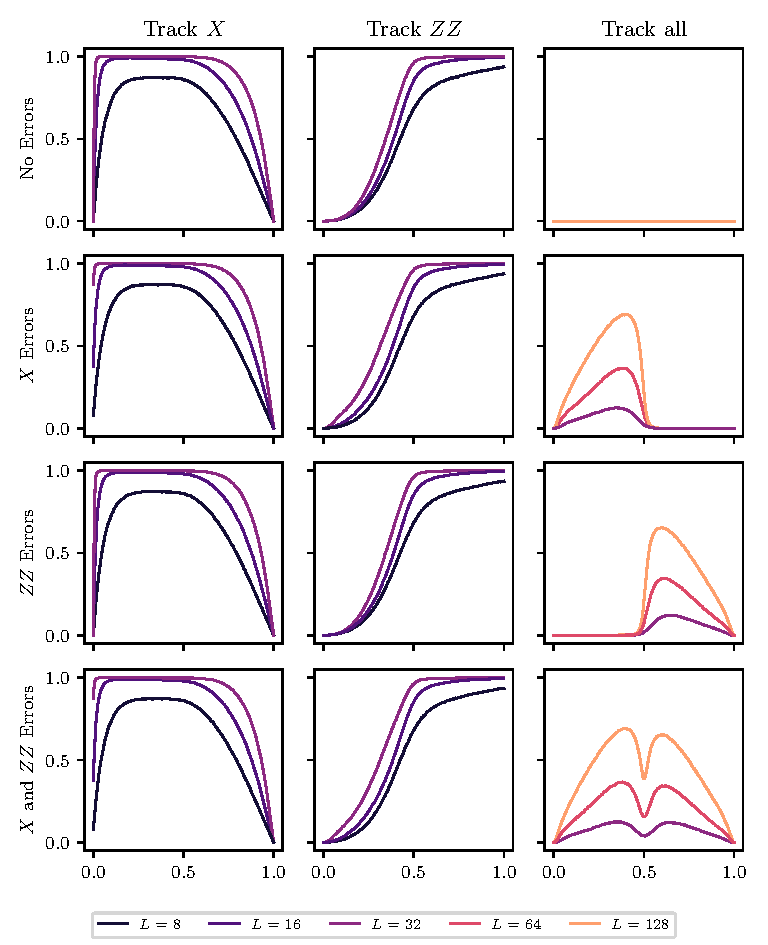
\includegraphics{minimal_mixing-4x3-inftyratio.pdf}
  \caption{Ratio of divergences in cross entropy to number of samples for the
    \enquote{minimal mixing} algorithm with
    different system sizes and
  periodic boundary conditions. To be able to adequately compare it to LXE the
different trackings and errors are shown in the same manner as in
\cref{fig:err-vs-tra}.}
  \label{fig:min_mix-inftyratio-4x3}
\end{figure}

  
As measure for how much contribution the algorithm has in the end, consider
\cref{fig:min_mix-svn_sigma_full-4x3}, where the von Neumann entropy of the
full density matrix of the reconstruction attempt is shown for all the various
previous cases.  We can see in the \enquote{Track X} column, that there is some
contribution from the algorithm itself, since we do not track the results from
$ZZ$ measurements, which would interfere with projections in $X$ towards the
regime where the initial cluster dies. 

\begin{figure}[p]
  \centering
  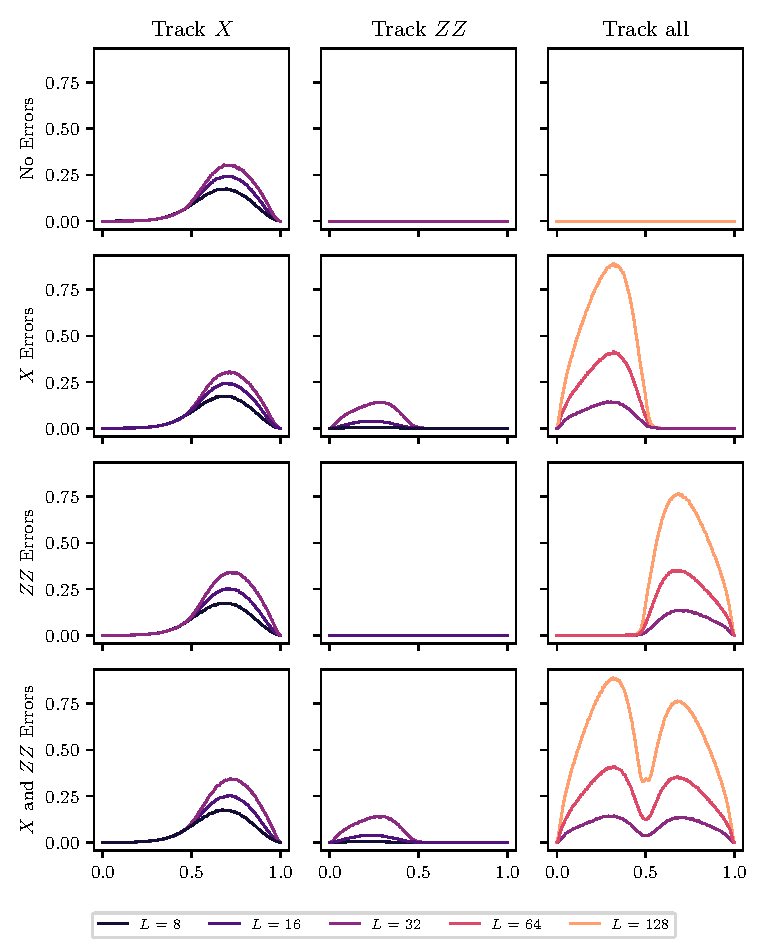
\includegraphics{minimal_mixing-4x3-svn_sigma_full.pdf}
  \caption{$S(\sigma)$ of full density matrix $\sigma$ 
  periodic boundary conditions. To be able to adequately compare it to LXE the
different trackings and errors are shown in the same manner as in
\cref{fig:err-vs-tra}}
  \label{fig:min_mix-svn_sigma_full-4x3}
\end{figure}

%\begin{itemize}
%  \item We would like to compare $\rho$, which is the \enquote{experiment}
%    (i.e. a quantum simulator), with $\sigma$, which is the classical
%    simulation.
%  \item The algorithm follows a similar structure to
%    \cite{liCrossEntropyBenchmark2023}, wherein we project the measurement
%    outcomes from $\rho$ onto $\sigma$ where it is possible. The difference
%    being that we do not start with orthogonal GHZ states, but with identical
%    GHZ states. That way, there will be no incompatible measurement as long as
%    there are no errors
%  \item but what if there are errors?
%  \item consider the case that an $X$-error occurred after a $ZZ$-measurement.
%  \item Half of the time we will get an incompatible projection, which would
%    project onto the zero-vector.
%  \item In those cases, we replace the stabilizer by $\mathds{1}$, where the
%    incompatibility was detected, instead of replacing it by the measurement
%    outcome or the projection.
%  \item This ensures that the subgroup condition still holds \emph{and} that
%    subsequent measurements on the same site cannot be interfered with, i.e.
%    that this qubits stabilizer is $\mathds{1}$ until it gets measured again.
%  %\item However, we rolled a nat20 on a sleight of hand skill check: in the
%  %  cases, where we \emph{would} get $\infty$, we replace $\sigma$ (whatever
%  %  it may be at this point) by $2^{-N} \mathds{1}$
%  %\item This is also in line with the general philosophy of the density
%  %  matrix. We do not know where the error occurred, and are therefore in a
%  %  mixture of all possible quantum states
%\end{itemize}

\clearpage
\subsection{Maximal Mixing}\label{sec:maximal-mixing}

The next algorithm is what we could call \enquote{maximal mixing}. 

\subsubsection{The algorithm}
It is
similar to the previously introduced algorithm with the caveat that we are now
not selectively removing stabilizer generators, but removing the whole
generating set. This is the most extreme method of how one could deal with the
noise, since now once we catch it, we in principle act as if no generator of
our generating set is to be trusted. Also, as the trivial group is always a
subgroup of any group (see \cref{sec:grouptheory}), and as the trivial group is
generated by the empty set (see \cref{defn:generators}), we should most
definitely ensure the fulfillment of the subgroup condition. The technical
details behind the implementation of this algorithm is given in
\cref{sec:other-dingers,alg:maximal-mixing}.

Note that this approach should also saturate the upper bound perfectly in the
noiseless case, since we only throw out generators when we encounter a mismatch
in the projections.
%\begin{itemize}
%  \item the first approach is what we'd call \emph{maximal mixing}.
%  \item The maginot line of no errors occuring is still a factor. However, each
%    time we encounter a discrepancy for the projections, we remove \emph{all}
%    the stabilizers in $\sigma$
%  \item since the trivial group is always a subgroup of any group (group
%    axioms), we still obey the subgroup rule
%  \item the technical details are laid out in \cref{alg:maximal-mixing}
%  \item most importantly, for a system with no errors, the bound is perfectly
%    saturated, with equality everywhere
%  \item when introducing errors, we lose this feature and start to become more
%    inaccurate.
%\end{itemize}

%\section{Results}\label{sec:upperbound-results}

%The results to the 
%\begin{itemize}
%  \item The results assume knowledge of \cref{fig:err-vs-tra} and the methods
%    used to obtain it.
%  \item Setup is the same as in \cref{ch:lxe}, in particular, the error model
%    is the same.
%  \item Now we do not have orthogonal initial states!
%\end{itemize}

\subsubsection{Results}
 
For the maximal mixing approach, we find that the first row of
\cref{fig:max_mix-svn_se-4x3} is almost identical to the corresponding plots in
\cref{fig:min_mix-svn_se-4x3} for the other processing algorithm.  This is due
to the fact that we have not introduced errors and the maximal mixing procedure
has no effect on this.
 
We also see that almost all the \enquote{Track $X$} or \enquote{Track $ZZ$}
columns are similar in appearance, except for \enquote{Track $ZZ$} when $X$
errors are present. We can infer an explanation for this by considering
\cref{fig:max_mix-svn_sigma_full-4x3}, where the von Neumann entropy of the
entire density matrices is shown.
 
For the \enquote{Track all} columns, we have values for the cross entropy that
are way smaller than with the previous algorithm.  When taking
\cref{fig:max_mix-inftyratio-4x3} into account, we notice that these
contributions are (almost) entirely from the post-processing algorithm we
chose.  For $X$ errors we have that the upper bound attains larger values for
$p \approx p_c$ with a slight slant to the left the converse is true for $ZZ$
errors, where the upper bound almost doesn't go back to the original curve.
 
For the noisiest system with $X$ and $ZZ$ errors, we have a combination of the
two effects Interestingly, the scaling at the critical point is linear, since
the peaks roughly double in magnitude with doubling the system size $L$.  This
is in contrast to the \enquote{ideal} case, where we have logarithmic scaling
at the critical point The peaks in the top right subplot are spaced evenly,
which is as expected with the doubling of system size.

\begin{figure}[p]
  \centering
  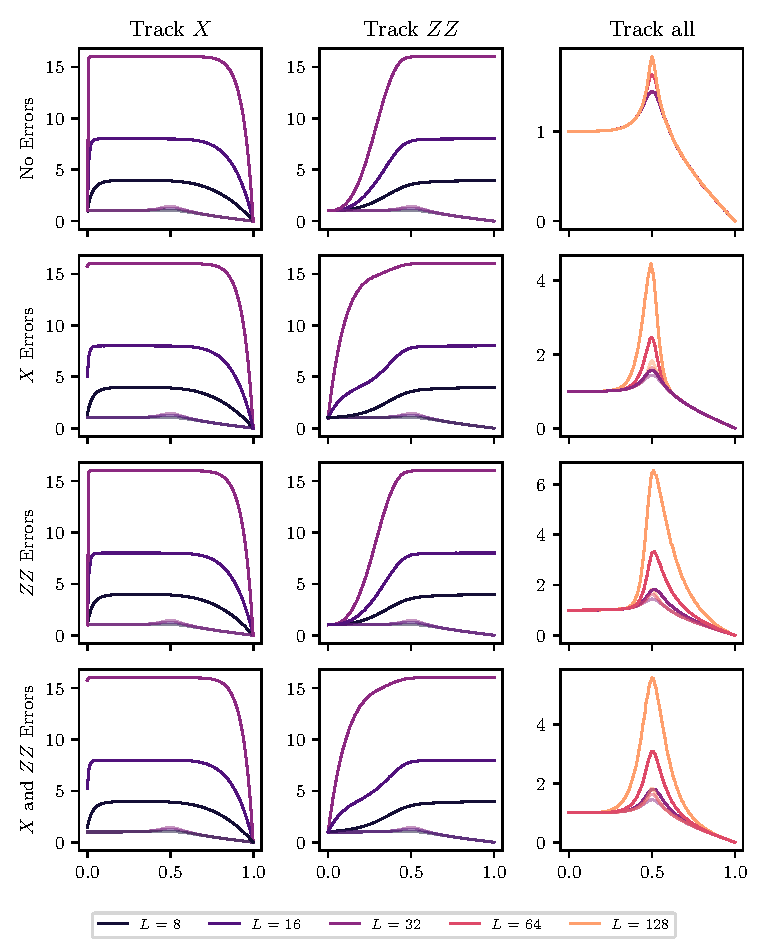
\includegraphics{extreme-rel-ent-4x3-svn_se.pdf}
  \caption{Cross Entropy and entanglement entropy of selected system sizes with
  periodic boundary conditions. To be able to adequately compare it to LXE the
different trackings and errors are shown in the same manner as in
\cref{fig:err-vs-tra}}
  \label{fig:max_mix-svn_se-4x3}
\end{figure}
  
For the infinity ratios, we have made progress: In the \enquote{Track all}
column, we find that we had no infinities almost everywhere.  However, there
are noticeable bumps in some of the plots. They are miniscule, but still there.
So miniscule that we can rule out the possibility of them substantially
contributing to the behavior shown in \cref{fig:max_mix-svn_se-4x3}.
Nonetheless, this shows that even with the most extreme measure of trying to
ensure the adherence to the subgroup condition, we still have some samples
bypassing it.  This undermines the fact that clusters emerge undetected, even
within the last measurement layers.  Consequently, we find that even when
compensating with the most extreme measures, we do not generally comply with
the subgroup condition.  This fact rules out any purely numerical approaches to
detect the phase transition.

\begin{figure}[p]
  \centering
  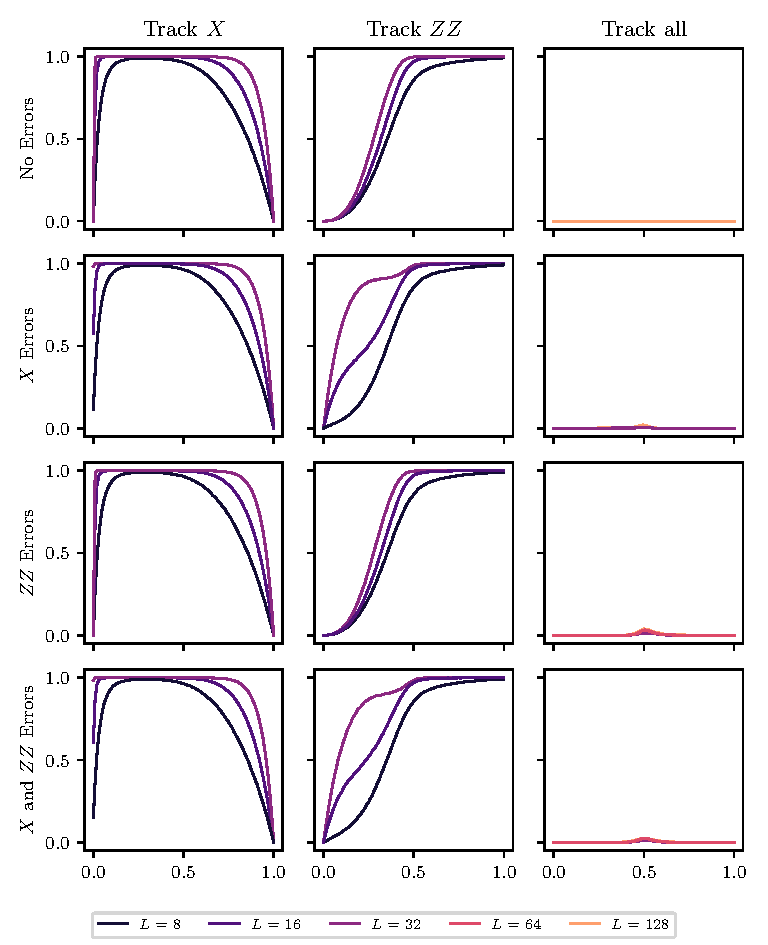
\includegraphics{extreme-rel-ent-4x3-inftyratio.pdf}
  \caption{Ratio of divergences in cross entropy to number of samples for
    different system sizes
  periodic boundary conditions. To be able to adequately compare it to LXE the
different trackings and errors are shown in the same manner as in
\cref{fig:err-vs-tra}}
  \label{fig:max_mix-inftyratio-4x3}
\end{figure}

When considering the full density matrix, we can again qualitatively measure
how good our approach was at the very end. We see that even though the
\enquote{mixedness} was set to the max, we never have an extremely large value
for the von Neumann entropy, as seen in \cref{fig:max_mix-svn_sigma_full-4x3}.

We find that for noisy systems, the algorithm did what it was designed to do,
namely, intercept errors. In the presence of $X$ errors we almost immediately
recover the whole group, but fail to recover the global $X$ stabilizer. This
shows itself in the \enquote{Track all} column of
\cref{fig:max_mix-svn_sigma_full-4x3}, where it goes to $1$ for $p\to 0$.  At
the critical point, there is a peak for large enough systems, since there we
have the highest impact of additional measurements of the competing kind.
Remarkably, just as in \cref{fig:min_mix-svn_sigma_full-4x3} we have
\enquote{$ZZ$ errors -- Track $ZZ$} be identically $0$. This follows from the
group structure. We never maximally mix. For the \enquote{Track $X$} column,
we just see the peak where the initial cluster dies, which was also present in
\cref{fig:min_mix-svn_sigma_full-4x3}.

\begin{figure}[p]
  \centering
  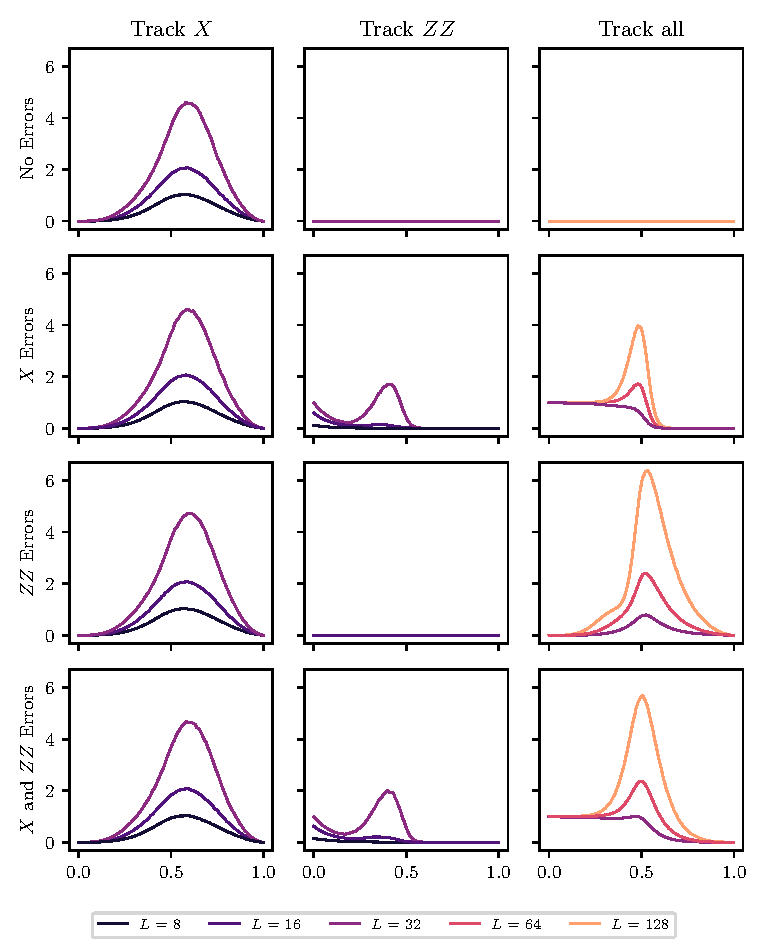
\includegraphics{extreme-rel-ent-4x3-svn_sigma_full.pdf}
  \caption{$S(\sigma)$ of full density matrix $\sigma$ 
  periodic boundary conditions. To be able to adequately compare it to LXE the
different trackings and errors are shown in the same manner as in
\cref{fig:err-vs-tra}}
  \label{fig:max_mix-svn_sigma_full-4x3}
\end{figure}

\clearpage
\section{Regularization}

We can see that, even though we chose our numerical algorithms in a way that
should mitigate the infinities, we still have them. Furthermore, the subgroup
check is a subtle way to incorporate once more what we try to avoid. Namely, we
want to find a density matrix, which is independent of the experimental density
matrix $\rho$. However, with the subgroup check, we implicitly introduce it
into our computation again. As we once more require knowledge of the full
density matrix, this would bring us right back to the sampling problem. In the
following we present two approaches to regularize the infinity appearing in the
cross entropy. These approaches require nothing but the numerically computed
density matrix $\sigma$. The first approach is one, which could be implemented
in a stabilizer simulator, which has the drawback of being exponentially worse
than the trivial upper bound $N$, among other things. The other is more
flexible, but lacks an efficient implementation in a stabilizer
simulation.\footnote{It is not definitive if there exists such an
implementation or not. For now, it does not exist yet.}
Note that these approaches are
designed to not need the subgroup condition to be fulfilled. As such, the
assumption of a noiseless last measurement layer could be restricted again to
include errors up to the end of measurements. 

Both of these approaches could be
the subject of further study, as the computational argument is one of
feasibility, but not possibility (i.e., it is possible, but at what
computational cost).

\subsection{Exponential Ansatz}
For the first regularization we choose an exponential Ansatz. The basic reasoning
behind this Ansatz is twofold. First, we want to ensure that the support of
$\sigma$ is large enough to contain the support of $\rho$. That is, what we
failed to achieve numerically, we attempt to achieve analytically. We want to
ensure that the classical processing step is only a function of the
measurement outcomes, $\sigma \equiv \sigma(\mathbf{m})$, and not the
experimentally obtained density matrix, which we implicitly had by checking the
subgroup condition on each run.

The second reason for this Ansatz in particular is the computability. Since we
are performing classical computations via the stabilizer formalism, we reduce
the memory requirements significantly. Storing a state of an $N$ qubit Hilbert
space is done in quadratic space complexity (see \cref{ch:mixed}). If we were
to write out the density matrix of, e.g., $N=100$ qubits explicitly, we would
have to deal with an exponentially large matrix. That is, if we choose $\sigma$
arbitrarily, 
we would be faced with the herculean task of diagonalizing a $2^{100} \times
2^{100}$ matrix when computing its logarithm, way beyond the scope of any reasonable computational
feasibility. By exponentiation we ensure that the logarithm \enquote{gets eaten
up} such that we are dealing with the density matrix itself with an additional
normalizing term.

As mathematical expression we may write\footnote{The factor of $\ln 2$ comes
  from the fact that we have the entropic quantities with base $2$. By a
leading factor of $1 /\ln 2$ this factor can be omitted.}
\begin{align}
  \tilde{\sigma} = \frac{\exp[\ln(2) \sigma]}{\Tr[\exp[\ln(2) \sigma]]}
.\end{align}
Substituting $\tilde{\sigma}$ back into the right hand side of
\cref{eq:kleins-ineq} we get
\begin{align}\label{eq:exp-ansatz}
  -\Tr[\rho\log\rho]\leq-\Tr[\rho\log\tilde{\sigma}] = -\Tr[\rho\sigma] +
  \log(\Tr[\exp[\ln(2)\sigma]])
.\end{align}
Note that the original $\sigma$ is still our classical reconstruction, i.e. a
density matrix in the stabilizer formalism. As $\sigma$ is therefore a product
commuting projectors, and with that a projector itself, we can once again
compute $-\Tr[\rho\sigma]$ efficiently. If $\rho=\sigma$, it recovers the
purity of $\rho$ with a negative sign, and if $\rho \perp \sigma$, then the trace is $0$. In a
sense, we here have recovered an inner product between density matrices, defined
as
\begin{align}
  \langle \rho, \sigma \rangle = \Tr[\rho\sigma]
.\end{align}
This inner product can be efficiently computed in the stabilizer formalism, as
we merely need to count projectors, and if they are orthogonal, the resulting
inner product is $0$. We remark that for density matrices, this inner product
is bounded with $\Tr[\rho\sigma] \in [0,1]$.

To efficiently compute the resulting upper bound from choosing the exponential
Ansatz, we need to resolve the logarithm in \cref{eq:exp-ansatz}. To this end
we proceed by first calculating the argument of the trace, which turns out to
yield the result of the trace as byproduct.

Since the density matrix of interest is, up to a prefactor, a projector, we
rewrite $\ln(2)\sigma$ as $c\mathbb{P}$ with some constant factor $c$.
By the matrixexponential we have
\begin{alignat*}{2}
  \exp[c\mathbb{P}] 
    = \sum_{k=0}^\infty \frac{\left(c\mathbb{P}\right)^k}{k!}
    &= \mathds{1} + \sum_{k=1}^\infty \frac{\left(c\mathbb{P}\right)^k}{k!}\\
    &= \mathds{1} + \mathbb{P}\sum_{k=1}^\infty \frac{c^k}{k!}
    &&\qquad{(\mathbb{P}^2 = \mathbb{P})}\\
    &= \mathds{1} + \mathbb{P}\left(\sum_{k=0}^\infty \frac{c^k}{k!} - 1\right)
    &&\qquad{\text{(shift index)}}\\
    &= \mathds{1} + \mathbb{P}\left(e^c -1\right) \\
    &= \mathds{1} + 2^{N-n}\sigma\left(2^{2^{n-N}}-1 \right) &&\qquad{(c =
      2^{n-N}\ln(2) \text{ and } \sigma = 2^{n-N}\mathbb{P}_s)}
.\end{alignat*}
We can then calculate the trace easily, since $\Tr[\mathds{1}] = 2^N$
and $\Tr[\sigma] = 1$. It follows that
\begin{align}
  \Tr[\exp[\ln(2)\sigma]] &= 2^N + 2^{N-n}\left(2^{2^{n-N}} -1 \right)
  \label{eq:trace-exp}
.\end{align}
Note that the parenthesis in \cref{eq:trace-exp} never vanish, but only
asymptotically reach $0$ in the thermodynamic limit. This is also the case if
one flips the sign, i.e. $\exp[-c\mathbb{P}]$, where one obtains
\begin{align}
  \Tr[\exp[\ln(2)\sigma]] &= 2^N + 2^{N-n}\left(1-2^{-2^{n-N}}\right)
.\end{align}
For both of these cases we have that the resulting upper bound is worse than
trivially assuming $N$, with diminishing fluctuations in $n$,
\begin{align}
  \log\left(\Tr[\exp[\ln(2)\sigma]]\right) &= \log(2^N +
  2^{N-n}\left(2^{2^{n-N}} -1 \right)) \geq N
.\end{align}

Since this Ansatz is worse than the trivial upper bound with variations in $n$
being small compared to the system size, we did not immediately see utility in
this approach. However, all quantities in the above calculations are
technically computable in the stabilizer simulator, and could thus be subject
of future study. 

\subsection{Rescaling probabilities}
The second regularization approach could be called the naive regularization
approach. We again want the support of $\sigma$ to span the entire Hilbert
space. With $\sigma$ being a product of projectors, it is a projector itself,
up to multiplicative factors. To complete the Hilbert space, we would need to
add the rest of the $2^{N}-2^{N-n}$ projectors needed, and rescale them in
order to put more (or less) weight on our prediction. Concretely,
we want $\sigma$ to have the form of
\begin{align}
  \tilde{\sigma} &= (1-\varepsilon)\sigma +  c\sum_{s \in
  \mathrm{ker}(\sigma)} \mathbb{P}_s \label{eq:complement-sigma}\\
&= (1-\varepsilon)\sigma +  \frac{\varepsilon}{\Tr[\sum_{s \in
\mathrm{ker}(\sigma)} \mathbb{P}_s]}\sum_{s \in
\mathrm{ker}(\sigma)} \mathbb{P}_s \label{eq:epsilon-over-trace}
,\end{align}
such that the diagonal form of $\sigma$ is
\begin{align}
  D_\sigma = \mqty(\dmat{1-\varepsilon,c,\ddots,c,c})
.\end{align}
This way, every basis vector of $H^{\otimes N}$ is included in $\sigma$ with a
weight of either $(1-\varepsilon)$ or $c$. As we want to ensure that
$\Tr[\tilde{\sigma}] =1$, $c$ is parametrized by $\varepsilon$. We now want to derive an
expression for $c(\epsilon)$, i.e. the trace in \cref{eq:epsilon-over-trace},
as well as a way to determine the constituents of the sum in
\cref{eq:complement-sigma}.

In principle, we need the sum in \cref{eq:complement-sigma} to go over all
orthogonal projections in the kernel of $\sigma$.
Since the support of $\sigma$ is fixed by the projectors onto the eigenspaces
of the tensor products of Pauli matrices contained in the generating set, we
need the orthogonal complement of each of them. Suppose we have the respective
signs of the generators $g_i$ in a bitstring $r_i$ of length $n$, i.e.
$\mathbf{r} \in \mathbb{F}^n_2$. We then write $\sigma$ as
\begin{align}
  \sigma = \frac{1}{2^N} \prod_{i=1}^n \left( \mathds{1}+(-1)^{r_i} g_i \right) 
.\end{align}
We then have a sum over all the combinations of values of $r_i$, which are
\emph{not} the original bitstring. We might write this as
\begin{align}
  \sum_{s\in\mathrm{ker}(\sigma)} \mathbb{P}_s = \sum_{\mathbf{r}' \neq \mathbf{r}} \frac{1}{2^n}\prod_{i=1}^n \left(
  \mathds{1} + (-1)^{r_i} g_i \right) 
.\end{align}
The subspaces of each of the above projectors is one-dimensional, and thus
their trace is $1$. Since there are $2^N$ total dimensions, and $2^{N-n}$ of
them are already in the support of $\sigma$, we have a total of $2^{N-n}\left(
2^n -1\right)$ additional projectors.\footnote{One can also arrive at this through
combinatorical arguments over the sign vector $\mathbf{r}$.} By rearranging and
by using the completeness relation, one can also reduce the number of
projectors needed to $\abs{\mathcal{S}_\sigma}$. However, the trace still
remains the same, since we want to rescale the missing diagonal entries
uniformly. This then yields
\begin{align}
  c = \frac{\varepsilon}{2^{N-n}\left( 2^n -1 \right) }
\end{align}
and thus
\begin{align}
  \tilde{\sigma} = (1-\varepsilon)\sigma + \frac{\varepsilon}{2^{N-n}\left( 2^n
  -1 \right) } \sum_{s\in\mathrm{ker}(\sigma)} \mathbb{P}_s
.\end{align}

Having determined a form for the auxilliary density matrix, we want to examine
it in the context of the cross entropy. It now becomes
\begin{align}
  -\Tr[\rho\log\sigma] = -\sum_n \matrixel{n}{\rho}{n} \log\lambda_n
\end{align}
with $\lambda_n =(1-\varepsilon)$ or $\lambda_n = \varepsilon
\left(2^{N-n}(2^n-1) \right)^{-1}$. While this appears to be better than the
diagonalization of a $2^{N} \times 2^{N}$ matrix, we still need to be aware
of -- or compute -- the representation of $\rho$ in the space, where $\sigma$
is diagonal.  Therefore, we do not quite dodge the task of handling an
exponentially large matrix.

%However, we can reduce this sum by realizing, that a projection onto \emph{one}
%of them halves the space which is projected onto. We can therefore build up the
%sum in the following way. First, we project onto the orthogonal space of the
%first generator, i.e.
%\begin{align}
%  \tilde{\mathbb{P}}^\perp_1 = \frac{1}{2}\left( \mathds{1} + (-1)^{1-r_1} g_1 \right) 
%.\end{align}
%Note that to ensure a uniform rescaling, we need to correct for the number of
%dimensions projected onto. In this case, we project onto a
%$2^{N-1}$-dimensional subspace.\footnote{This is a first indicator that this
%approach gets finicky.} Additionally, with said prefactor this is not a genuine
%projector anymore, since $\tilde{\mathbb{P}}^2 \neq \tilde{\mathbb{P}}$.
%
%The next one in the sum is the projector onto the space of $g_1$ multiplied by
%the orthogonal complement of $g_2$,
%\begin{align}
%  \tilde{\mathbb{P}}^\perp_2 = \frac{1}{2^{N-1}}\left(\mathds{1} + (-1)^{r_1} g_1  \right)
%  \left( \mathds{1} + (-1)^{1-r_2} g_2 \right) 
%.\end{align}
%This continues for all generators of the generating set.
%This way, we only need $\abs{\mathcal{S}_\sigma}$ projectors in the sum. 
%Since they take the form of
%\begin{align}
%  \mathbb{P}_s = \frac{1}{2}\left( \mathds{1} + s \right) 
%\end{align}
%with $s \in \mathcal{P}_N$, their trace is
%\begin{align}
%  \Tr[\mathbb{P}_s] = \frac{1}{2} 2^N = 2^{N-1}
%.\end{align}
%We argued that we only need $\abs{\mathcal{S}_\sigma}$ projectors in the sum.
%Therefore, \cref{eq:epsilon-over-trace} becomes
%\begin{align}
%  \tilde{\sigma} &= (1-\varepsilon)\sigma +
%  \frac{\varepsilon}{\abs{\mathcal{S}_\sigma}2^{N-1}}\sum_{s \in
%  \mathrm{ker}(\sigma)} \mathbb{P}_s 
%,\end{align}
%given that we choose the projectors with the above described method.


%There are $n$ generators for $\sigma$.
%
%\begin{itemize}
%  \item eigentlich sinds $2^N - 2^{N-n}$ verschiedene orthogonale projektionen,
%    die zu machen sind
%  \item gibt cleveren algorithmus wie man das reduzieren kann:
%    \begin{enumerate}
%      \item orthogonales komplement zum projektor auf den ersten
%      \item projektor auf den ersten, multipliziert mit projektor auf
%        orthogonales komplement vom zweiten
%      \item projektor auf ersten mal projektor auf zweiten mal o.k. von
%        projektor auf dritten
%      \item etc\ldots
%    \end{enumerate}
%  \item damit reduziert man erheblich, man braucht dann nur so viele wie man
%    generatoren hat, also $n$, anstatt exponentiell viele
%  \item nur doof, dass es auch daf\"ur keine gute methode gibt im stabilizer zu
%    handlen
%  \item kann sich ja der n\"achste masterand ransetzen?
%\end{itemize}

\clearpage
\section{Summary}
In this chapter we investigated the utility of Klein's inequality to detect the
entanglement transition in the projective transverse-field Ising model. 
The idea behind this approach is from
\citeauthor{garrattProbingPostmeasurementEntanglement2023} in
\cite{garrattProbingPostmeasurementEntanglement2023}, where it was numerically
studied with MPS simulations for Haar-random hybrid circuits. To adapt to our
system, we derived the inequality in the stabilizer formalism. We then employed
the derived expressions in a stabilizer simulation of the PTIM, where we
investigated different numerical post-processing approaches. We then concluded
the chapter by suggesting regularizations to deal with unwanted infinities.
%OThis
%inequality has first been employed in this manner by
%\citeauthor{garrattProbingPostmeasurementEntanglement2023} in
%\cite{garrattProbingPostmeasurementEntanglement2023}. 
%\section*{some relevant references}
%\begin{enumerate}
%  \item \textcolor{red}{\citetitle{aaronsonImprovedSimulationStabilizer2004}
%      fuck why didn't i read it in its entirety earlier: section 7 does the
%    job\ldots}
%  \item \citetitle{veitchResourceTheoryStabilizer2014}, entropic quantities of
%    magic states; quantifying non-stabilizerness. This paper is with gottesman
%    himself, so i thought it might be interesting to study. 
%  \item \citetitle{niekampEntropicUncertaintyRelations2012}, more or less what
%    it says. No regularization scheme or whatever. I think stabilizers are
%    mentioned tangentially, thats why i found it.
%  \item \citetitle{lashkariRelativeEntropiesConformal2014}, $\leftarrow$ me
%    grasping for straws.
%  \item \citetitle{leonePhaseTransitionStabilizer2024}, very recent, not too
%    particularily relevant to our stuff as far as i can tell.
%  \item \citetitle{wuEntanglementUpperBound2011} idfk\ldots
%  \item \citetitle{vedralEntanglementMeasuresPurification1998} one of the more
%    promising papers i've come across. probably helpful in proving the failure
%    of the na\"ive approach. However, it was published in 1998. It most likely
%    has nothing to do with stabilizers.
%  \item \citetitle{lindenQuantumEntropyCone2013}, probably some interesting
%    stuff in there, but not the thing i want.
%  \item \citetitle{buExtremalityStabilizerStates2024}, this paper is where most
%    of my confusions come from. 
%\end{enumerate}


\chapter{Classical \ Simulation \ of \ Stabilizer \ Circuits}
\label{ch:mixed}
\epigraph{Always programming a new type of antidote in your perimeter}{
\citeauthor{quasimotoDiscipline99Pt2000}
%on \citefield{quasimotoDiscipline99Pt2000}{title}
}

In this chapter we present the simulation algorithm and 
the modifications to the existing infrastructure (cf. ref.
\cite{langCliffordCircuitSimulator2022}) that
were necessary for the numerical experiments of this thesis. Usually, these
would fall into the \emph{Methods} sections of the respective
chapters. However, the modifications were extensive enough to warrant the
dedication of an entire chapter to them. We will first briefly introduce the
simulation algorithm based on the results from Gottesman and Knill
\cite{gottesmanHeisenbergRepresentationQuantum1998}, and Gottesman and Aaronson
\cite{aaronsonImprovedSimulationStabilizer2004}. Then, we briefly present
the functions
necessary for computing the linear cross entropy $\chi$, from \cref{ch:lxe}, as
this was only a small addition. We
then finish off with the larger discussion of mixed states in the stabilizer
formalism and the realizations of the mixed state simulation algorithms, as
well as the functions for the various entropic quantities, implementing our
results from \cref{sec:rel-ent-stab}.

%Ref. \cite{aaronsonImprovedSimulationStabilizer2004} will need to do some heavy
%lifting in giving primers on stabilizer simulation.
%
%It will later prove useful to implement mixed states into the existing
%stabilizer simulator. As of yet, this does not exist.
%
%In this paper \cite{audenaertEntanglementMixedStabilizer2005} they present an
%algorithm to perform a partial trace on a stabilizer state. They need an
%auxilliary algorithm, the Reduced row echelon form algorithm. I think this is a
%promising approach, but needs implementation of the RREF and the ptrace
%algorithm. From what I've seen, the first one is going to take longer than the
%second to implement. Maybe look for this kind of alg in the existing codebase?
%
%Note from 10 minutes later: its basically what we already had, only a bit more
%formalized. 
%
%Lecture notes on stabilizers: \cite{arabLectureNotesQuantum2024}
%
%This chapter serves as a primer on the nitty-gritty details of simulating
%stabilizer circuits on a classical computer. As already touched on in
%\cref{ch:basics}, according to the \emph{Gottesman-Knill Theorem} we can
%perform efficient classical simulations of quantum circuits using only Clifford
%gates. In the following sections we will introduce the so-called tableau
%algorithm, which allows simulations in polynomial time, and expand it to
%properly deal with mixed states. We assume the reader to be familiar with the
%corresponding sections in \cref{sec:stab-basics}.

\subsubsection*{A computer science primer}
%%% WAS HIER URSPRÜNGLICH MAL STAND:
% This chapter addresses classical computation and algorithms, focussing on the
% simulation of a particular class of quantum circuits using classical computers.
% As such, it will necessarily feature terminology commonly associated with the
% field of computer science. While this thesis as a whole is a work on natural
% science – i.e. theoretical physics – our focus lies more on simulations as a
% tool rather than as the primary object of study. Nonetheless, to ensure
% clarity, we will briefly introduce key terminology from computer science.
%%%
This chapter is something of an outlier compared to the other chapters. While
the previous part of this work pertains to \emph{natural} science -- namely,
theoretical physics -- where simulations served us as a tool rather than as the
primary object of study, a substantial portion of this thesis has been
dedicated to expanding an existing stabilizer simulator to deal with new
problems (cf.  \cref{sec:lxe-numeric,sec:rel-ent-stab,sec:upperbound-numerics}). As a result, our
discussion thereof will necessarily feature
%cursed language devised by the utterly deranged: computer scientists. To
%prepare for this, we will introduce some of its vocabulary here.
terminology commonly associated with the field of \emph{computer} science.
To ensure clarity, we will briefly introduce key computer science concepts
relevant to our discussion.  

The first concept we introduce is asymptotic behavior, along with the so-called
\emph{Big }$\mathcal{O}$ notation. It is not exclusive to computer science as such, as we
often deal with asymptotic behavior in physics as well.  In computer science,
the Big $\mathcal{O}$ notation is used to describe the space (i.e. data storage) and
time requirements of algorithms with increasing input size. The notation is
defined precisely in \cref{defn:bigo-theta}.
\begin{defn}[$\Theta$ and $\mathcal{O}$ notation
  \cite{cormenIntroductionAlgorithms2009}]\label{defn:bigo-theta}
  Let $g(n)$ be a positive function. Then $\Theta(g(n))$ is the set of
  functions 
  \begin{align*}
    \Theta(g(n)) = \left\{ \ f(n) \mid \liminf_{n\to\infty} \frac{f(n)}{g(n)} > 0 \
    \wedge \ \limsup_{n\to\infty} \frac{f(n)}{g(n)} < \infty \ \right\}
  .\end{align*}
  Similarly, $\mathcal{O}(g(n))$ is the set of functions 
  \begin{align*}
    \mathcal{O}(g(n)) = \left\{ \ f(n) \mid 
    \limsup_{n\to\infty} \frac{f(n)}{g(n)} < \infty \ \right\}
  .\end{align*}
\end{defn}
We will later see some examples of this notation in use. For now it suffices to
note that different problems and the algorithms we use to solve them (or verify
the validity of a solution) are grouped into a variety of \emph{complexity
classes}. For instance, an algorithm is said to scale polynomially (in time) if
its asymptotic behavior is $\mathcal{O}(n^\alpha)$ with $\alpha \geq 1$, and
exponentially if it is $\mathcal{O}(2^n)$. These classes constitute an
important subfield in theoretical computer science in the form of
complexity theory, where numerous classes exist.\footnote{A continuously
updated list can be found in \cite{ComplexityZoo}.} The two examples from above
fall in the classes \textsf{P} (polynomial time) and \textsf{EXP} (exponential
time) respectively.  While there are lots of caveats to this highly simplified
explanation, a deeper examination of complexity theory lies beyond the scope of
this thesis. However, the key takeaway is summarized in
\cref{defn:efficient-alg}.
\begin{defn}[Algorithmic efficiency \cite{ComplexityZoo}]\label{defn:efficient-alg}
  A problem is considered efficiently solvable on a classical computer if it
  belongs to the complexity class \textsf{P}.
\end{defn}
Having laid out these foundational concepts, we can now delve deeper into the
subtleties of stabilizers and the problem of simulating stabilizer
circuits, potentially gaining a new appreciation for their intricacies.

\section{Consequences of the Gottesman-Knill theorem}\label{sec:sim-stab}
In this section we explore the implications of \cref{thm:gottesman-knill} and
provide a proper introduction to the simulation algorithm that forms the
foundation for the numerical experiments in this thesis.  In particular, we
present the \emph{tableau algorithm}, as proposed by Aaronson and Gottesman in
\cite{aaronsonImprovedSimulationStabilizer2004}.  Consequently, this section
draws largely from outside sources, namely Refs.
\cite{aaronsonImprovedSimulationStabilizer2004, arabLectureNotesQuantum2024,
gottesmanStabilizerCodesQuantum1997,
gottesmanHeisenbergRepresentationQuantum1998}. As this following section serves
to introduce the computational algorithms based on the stabilizer formalism, it
can (and should) be read as a sequel to \cref{sec:stab-basics}.
%This section provides an introduction to the tableau algorithm. It can (and
%should)
%be read as the sequel to \cref{sec:stab-basics}. Note that this section is
%based on the work of \citeauthor{aaronsonImprovedSimulationStabilizer2004} in
%\cite{aaronsonImprovedSimulationStabilizer2004}.

We begin by recalling that the stabilizer group does not need to be stored in
full to unambiguously describe the state. Since the stabilizer group is finite,
its structure can be fully encapsulated by storing only its \emph{generators}
in memory. This reduces the amount of data to be stored to memory from $2^n$
to $n$, owing to the well-known fact from group theory that a finite group $G$
has a generating set of size $\log \abs{G}$. That is, an $n$-qubit pure state
$\ket{\phi}$ with stabilizer group $S\left(\ket{\phi}\right)$ has a generating
set of size $\log 2^n = n$.

To determine the actual memory requirements we examine the generators
themselves.  Each generator consists of an array of $n$ Pauli matrices and a
sign. Since there are $4$ Pauli matrices (including the identity), we require 2
bits to encode each of them, along with an additional bit for the sign.
Consequently, the memory requirements for encoding a pure state in the
stabilizer formalism is $n(2n+1)$. In other words, storing only the stabilizer
generators reduces the space complexity of stabilizer simulations from
$\mathcal{O}\left( 2^n \right)$ to $\mathcal{O}\left( n^2 \right)$.

For practical purposes, these bits can be assorted to two $n\times n$ matrices
and a vector containing the $n$ signs. This way of writing the generators is
called the \emph{Tableau Representation}. As an example, consider the state
$\ket{\phi}=\ket{0000}$, which is stabilized by Stab$(\ket{\phi}) = \langle
Z_1, Z_2, Z_3, Z_4\rangle$. The stabilizer tableau $\mathcal{T}$ of
$\ket{\phi}$ is then given by
\begin{align}\label{eq:stabtab}
\mathcal{T}_{\ket{\phi}} = 
\left[
  \begin{array}{cccc|cccc|c}
    0 & 0 & 0 & 0 & 1 & 0 & 0 & 0 & 0 \\
    0 & 0 & 0 & 0 & 0 & 1 & 0 & 0 & 0 \\
    0 & 0 & 0 & 0 & 0 & 0 & 1 & 0 & 0 \\
    0 & 0 & 0 & 0 & 0 & 0 & 0 & 1 & 0
  \end{array}
\right]
%\left[
%  \begin{array}{cccc|cccc|c}
%    \multicolumn{4}{c|}{\underbrace{
%    \begin{matrix}
%    0 & 0 & 0 & 0 \\
%    0 & 0 & 0 & 0 \\
%    0 & 0 & 0 & 0 \\
%    0 & 0 & 0 & 0
%    \end{matrix}}_{X\text{-matrix}}} &
%    \multicolumn{4}{c|}{\overbrace{
%    \begin{matrix}
%    1 & 0 & 0 & 0 \\
%    0 & 1 & 0 & 0 \\
%    0 & 0 & 1 & 0 \\
%    0 & 0 & 0 & 1
%    \end{matrix}}^{Z\text{-matrix}}} &
%    \underbrace{
%    \begin{matrix}
%    0 \\
%    0 \\
%    0 \\
%    0
%    \end{matrix}}_{\text{signs}}
%  \end{array}
%  \right]
.\end{align}
Each row in \cref{eq:stabtab} represents a generator of Stab$(\ket{\phi})$. The
first four columns are the $X$-matrix, the next four are the $Z$-matrix and the
last column represents the sign. The $i$-th column of the $X$ and $Z$ matrix
encode the Pauli matrix at position $i$ in the tensor product of the
corresponding generator, where $00\equiv I$, $01\equiv Z$, $10\equiv X$, and
$11\equiv Y$. 

At this point, we have merely stored the state in memory. However,
\cref{thm:gottesman-knill} implies that simulations of stabilizer cicruits can
also be done efficiently on a classical computer. As stated in
\cref{defn:efficient-alg}, for an algorithm to be
considered \enquote{efficient}, it must have polynomial time complexity.
Thus, the Gottesman-Knill theorem can be rephrased to state that the bits encoding
$\ket{\phi}$ can be updated in polynomial time after a Clifford gate is
applied to $\ket{\phi}$. Before we show this, let us first consider how the individual
gates act on our generator tableau. 
\begin{alg}[Application of Clifford gates to stabilizer
  tableau]\label{alg:cliff-gates-alg1}
  The following modifications have to be applied to the stabilizer tableau
  after the application of
  \begin{itemize}
    \item $H$ to qubit $a$:

      Swap column $a$ of the $X$ matrix with the $a$-th column of the
      $Z$-matrix.
    \item $S$ to qubit $a$:

      Modify column $a$ of the $Z$-matrix such that the
      new $z_{ia} = z_{ia} \texttt{XOR} x_{ia}$, i.e. apply bitwise
      \texttt{XOR} from column $a$ of $X$ into column $a$ of $Z$.
    \item CNOT from control $a$ to target $b$:
     
      Apply bitwise \texttt{XOR} from
      column $a$ to $b$ of $X$, and from column $b$ to column $a$ of $Z$.
    \item Random or deterministic outcome of computational basis measurement on
      qubit $a$:

      The outcome is deterministic iff. column $a$ of the $X$-matrix is all 0s.
    \item Measurement of qubit $a$ with a random outcome

      Let $x_{ia}=1$. We first apply bitwise \texttt{XOR} from row $i$ into any
      subsequent row $j$, where $x_{ja}=1$. We then set row $i$ to $0$
      everywhere, except $z_{ia}=1$ and set the sign to $0$ or $1$ randomly.
  \end{itemize}
\end{alg}
These rudimentary algorithms follow the rules of the stabilizer formalism, as
laid out in \cref{sec:stab-basics}. Let us now consider the performance of
the algorithms in \cref{alg:cliff-gates-alg1}.

\begin{thm}[Simulating stabilizer gates]\label{thm:sim-stab-comp}
  Simulating a Clifford gate on an $n$-qubit stabilizer state requires $\Theta(n)$
  time, while a measurement gate is simulated in $O(n^2)$ or $O(n^3)$ time for
  random and deterministic outcomes respectively.
\end{thm}
\begin{proof}
  We already know that an $n$-qubit stabilizer state $\ket{\phi}$ can be represented as an
  $n\times(2n+1)$ tableau $\mathcal{T}$, where the rows are the $n$ generators in the
  afforementioned $(2n+1)$-bit representation. Any computational basis state can
  thus be represented by
  \begin{align}
    \mathcal{T} = 
    \left[
      \begin{array}{cccc|cccc|c}
        0 & 0 & \ldots & 0 & 1 & 0 & \ldots & 0 & \pm \\
        0 & 0 & \ldots & 0 & 0 & 1 & \ldots & 0 & \pm \\
        \vdots & \vdots & \ddots & \vdots & \vdots & \vdots & \ddots & \vdots & \vdots \\
        0 & 0 & \ldots & 0 & 0 & 0 & \ldots & 1 & \pm
      \end{array}
    \right]
  ,\end{align}
  where $Z$ and $I$ are encoded as $01$ and $00$ respectively, and $\pm$ is a
  placeholder for either $0$ or $1$ depending on the sign. Simulating a
  Clifford gate $U$ on $\ket{\phi}$ maps $g_i$, that is, the $i$-th row of
  $\mathcal{T}$, to $U g_i U$. As discussed in \cref{alg:cliff-gates-alg1},
  this operation updates at most two columns. Therefore, simulating $U$ takes
  $\Theta(n)$ time.

  To show the scaling behavior of measurements we consider computational basis
  measurements on qubit $a$, $Z_a$, without loss of generality.\footnote{We can
    consider those without loss of generality, since we can always apply
    $\mathcal{O}(n)$ unitaries to change basis in $\Theta(n)$ time, which
  doesn't affect the scaling behavior of $\mathcal{O}(n^2)$.} Each individual
  qubit in $\ket{\phi}$ is either in a computational basis state $\ket{0}$ or
  $\ket{1}$, where we have a deterministic outcome, or in a superposition of
  both states with equal amplitude, where either outcome is random with
  probability $p=1 / 2$. Recall from \cref{sec:stab-basics} that the process of
  determining the type of outcome (random or deterministic) is done by checking
  the commutation relations between the measurement operator and the generators
of $\ket{\phi}$. If some generator $g_k$ anti-commutes with $Z_a$, i.e.
\[ \{g_k, Z_a\} =0 \quad{\text{or}}\quad [g_k, Z_a] \neq 0,\]
the outcome is random,
  otherwise it is deterministic (this implies a scaling of $\mathcal{O}(n)$
  already, since we go through the entire matrix in the worst case). We now
  consider these cases separately.
  
  \par{Case 1, random outcome:}
  Let $g_k$ be a stabilizer generator with $\{g_k, Z_a\}=0$, implying a random
  outcome. As the outcome, we randomly choose $x\in\{0,1\}$. We then multiply
  any subsequent rows that anticommute with $Z_a$ by $g_k$ in order for them to
  commute with $Z_a$. We then replace $g_k$ by $\pm Z_a$ depending on the
  random outcome. Since this algorithm takes up to $n$ row multiplications,
  the runtime scales with $\mathcal{O}(n^2)$.

  \par{Case 2, deterministic outcome:}
  If we did not find an anticommuting generator, we know that our stabilizer
  group contains $Z_a$. However, this does not necessitate $Z_a$ being in the
  generating set.
  We thus need to modify
  $\mathcal{T}$ such that its row space contains $\left( 00\cdots 0_a\cdots 0\mid
  00\cdots 1_a \cdots 0 \mid \pm \right) = \pm Z_a$ and then read out the signs
  vector, which is the result. This is done by Gaussian
  elimination, which requires $\mathcal{O}(n^3)$ time.
\end{proof}
This proof, in principle, also proves \cref{thm:gottesman-knill}, since the
simulation of any of a circuit's constituents is in \textsf{P}. Consequently, a
finite number $m$ of them will be in $\mathcal{O}(mn^\alpha)$, and thus also in
\textsf{P}.

\subsection{The Aaronson-Gottesman Algorithm}\label{sec:tableau}
In the previous section we have shown that measurements take $\mathcal{O}(n^3)$
time in practice. However, Aaronson and Gottesman showed in
\cite{aaronsonImprovedSimulationStabilizer2004} that with the cost of a factor
2 increase in memory requirements we can improve measurements to have
quadratic time complexity $\mathcal{O}\left(n^2\right)$, independent of
\enquote{outcome type}. In particular, for each of the $n$ stabilizer
generators we store a destabilizer (also equivalently referred to as
antistabilizer) generator, which are also tensor products of Pauli operators.
These $2n$ operators together generate the full $n$-qubit Pauli group
$\mathcal{P}_n$.

The tableau idea applied in \cref{eq:stabtab} can be expanded into
\begin{align}\label{eq:new-stabtab}
  \mathcal{T}_{\ket{\phi}} = 
  \left[
    \begin{array}{ccc|ccc|c}
      x_{11} & \cdots & x_{1n} & z_{11} & \cdots & z_{1n} & r_1 \\
      \vdots & \ddots & \vdots & \vdots & \ddots & \vdots & \vdots \\
      x_{n1} & \cdots & x_{nn} & z_{n1} & \cdots & z_{nn} & r_n \\ \hline
      x_{(n+1)1} & \cdots & x_{(n+1)n} & z_{(n+1)1} & \cdots & z_{(n+1)n} & r_{n+1} \\
      \vdots & \ddots & \vdots & \vdots & \ddots & \vdots & \vdots \\
      x_{(2n)1} & \cdots & x_{(2n)n} & z_{(2n)1} & \cdots & z_{(2n)n} & r_{2n}
    \end{array}
  \right]
\end{align}
for an arbitrary stabilizer state $\ket{\phi}$. The first $n$ rows represent
the newly introduced destabilizer states, while the last $n$ rows constitute
the tableau of stabilizers we have already discussed. For later convenience, an
additional $(2n+1)$st row is added to the tableau. A minimal example of the
generalized tableau is the state $\ket{00}$, which has
\begin{align}\label{eq:new-stabtab-example}
  \mathcal{T}_{\ket{00}} = 
  \left[
    \begin{array}{cc|cc|c}
      1 & 0 & 0 & 0 & 0 \\
      0 & 1 & 0 & 0 & 0 \\ \hline
      0 & 0 & 1 & 0 & 0 \\
      0 & 0 & 0 & 1 & 0 \\ \hline
      0 & 0 & 0 & 0 & 0 
    \end{array}
  \right]
.\end{align}
A quick remark on notation: we will refer to the $i$th row of $\mathcal{T}$ by
$R_i$, where it is clear from the respective context if the row refers to a
stabilizer or destabilizer generator. If we explicitly refer to one of them, we
write $g_i$ for the $i$th stabilizer generator and $h_i$ for the $i$th
antistabilizer generator. Matrix elements of the $X$ and $Z$ matrices are
denoted by $x_{ab}$ and $z_{ab}$ respectively. Entries of the sign vector are
denoted by $r_i$ (cf. \cref{eq:new-stabtab}).

Although it is simply stated, it is not immediately obvious how (a) we choose
destabilizer generators, and (b) how this improves the scaling of measurements.
For now we say that the simulation algorithm starts in the state
$\ket{0}^{\otimes n}$, where the initial tableau is taken as the $n$-qubit
generalization of \cref{eq:new-stabtab-example}. Any other stabilizer state can
then be arrived at via Clifford or Pauli measurement gates. The former can be
implemented as follows.
\begin{alg}[Improved simulation of Clifford gates]\label{alg:tab-clifford}
  Let $\oplus$ denote bitwise \verb|XOR|. The implementations are
  \begin{itemize}
    \item CNOT from control $a$ to target $b$:

      $\forall i \in \{1,\ldots,2n\}$ $r_i := r_i \oplus x_{ia}z_{ib}\left(
      x_{ib} \oplus z_{ia} \oplus 1 \right)$, $x_{ib} := x_{ib} \oplus x_{ia}$,
      and $z_{ia} := z_{ia}\oplus z_{ib}$.
    \item $H$ on qubit $a$:

      $\forall i \in \{1,\ldots,2n\}$ $r_i := r_i \oplus x_{ia}z_{ia}$, then
      swap $x_{ia}$ and $z_{ia}$.
    \item $S$ on qubit $a$:

      $\forall i \in \{1,\ldots,2n\}$ $r_i := r_i \oplus x_{ia}z_{ia}$, then
      set $z_{ia}$ to $z_{ia} \oplus x_{ia}$.
  \end{itemize}
\end{alg}
We know from earlier considerations that simulating measurement gates,
requires the multiplication of
generators. To this end, we introduce 
a subroutine called \texttt{rowsum(h,i)}.
It updates the $h$-th generator to be $h+i$
and keeps track of the phase $r_h$.
Its implementation is given in \cref{alg:rowsum}.
\begin{alg}[rowsum]\label{alg:rowsum}
  First we define a function $g(x_1, z_1, x_2, z_2)$ taking 4 bits as input and
  outputting the exponent of the imaginary unit $i$ after $x_1 z_1$ and $x_2 z_2$ are multiplied.
  We focus on four cases explicitly, namely
  \[
  \begin{array}{ccc}\toprule
      x_1 & z_1 & g(x_1,z_1,x_2,z_2) \\ \midrule
      0 & 0 & 0 \\
      0 & 1 & x_2\left( 1-2z_2 \right) \\
      1 & 0 & z_2\left( 2x_2-1 \right) \\
      1 & 1 & z_2 - x_2 \\ \bottomrule
  \end{array}
  \]
  For the rowsum routine we set $r_h$ to $0$ if
  \begin{align}\label{eq:congruentdings}
    2r_h + 2r_i + \sum_{j=1}^n g\left(x_{ij},z_{ij},x_{hj},z_{hj}\right) \equiv
    0 \text{ (mod } 4)
  .\end{align}
  or set $r_h$ to $1$ if the sum in \cref{eq:congruentdings} is congruent to
  $2$ mod $4$. Next, we set $x_{hj}$ to $x_{ij}\oplus x_{hj}$ and $z_{hj}$ to $z_{ij}
  \oplus z_{hj}$ for all $j$, where $\oplus$ denotes bitwise \verb|XOR|.
\end{alg}
Next it will prove useful to define the \emph{symplectic inner product} between
two Pauli operators $A$ and $B$ in tableau representation as
\begin{align}\label{eq:symp-inner-prod}
  A\cdot B = x_{a1}z_{b1} \oplus \cdots \oplus x_{an}z_{bn} \oplus x_{b1}
  z_{a1} \oplus \cdots \oplus x_{bn}z_{an}
.\end{align}
This inner product is $0$ if $A$ and $B$ commute and $1$ if they anti-commute.

Equipped with rowsum and the symplectic inner product, we can now examine the
simulation of measurement gates.
\begin{alg}[Improved simulation of Measurement gates]\label{alg:tab-measure}
  Suppose we measure $\hat{O}$. As a $0$th step,
  check if there exists a $p\in\{n+1,\ldots,2n\}$ (the stabilizer
  generators) such that $[\hat{O},R_p] \neq 0$. This can be done by
  multiplication with respect to \cref{eq:symp-inner-prod}. Then there are two
  cases:

  Case 1, such a $p$ exists. First, call rowsum($i,p$) for all $i \in
  \{1,\ldots,2n\}$ such that $i\neq p$ and $[\hat{O},R_i] \neq 0$. Next,
  set the $(p-n)$th row equal to the $p$th row. Then, set row $p$ equal to
  $\hat{O}$ and set $r_p$ to 0 or 1 with equal probability. Finally, return
  $r_p$ as measurement outcome.

  Case 2, such a $p$ does not exist. First, set the entire $(2n+1)$st row (the one
  added for convenience earlier) to 0. Next, call rowsum($2n+1, i+n$) for all
  $i\in\{1,\ldots,n\}$ (the destabilizer generators) such that
  $[\hat{O},R_i]\neq 0$. Finally, return $r_{2n+1}$ as measurement outcome. 
\end{alg}

With \cref{alg:tab-clifford,alg:rowsum}, all possible allowed modifications to
the stabilizer tableau $\mathcal{T}$ are defined. \Cref{prop:comm-tab} collects
some symmetries of this simulator. That is, some commutation relations are
invariant under operations of the Aaronson-Gottesman tableau algorithm. It is
these relations we want to keep intact, when setting out to expand the existing
simulator with more functionalities.
\begin{prop}[Invariants of the tableau algorithm]\label{prop:comm-tab}
  The following are invariant under operations of the tableau algorithm
  \begin{enumerate}
    \item $R_{n+1},\ldots,R_{2n}$ generate $S(\ket{\phi})$, and $R_1, \ldots,
      R_{2n}$ generate $\mathcal{P}_n$.
    \item $R_1, \ldots, R_n$ commute.
    \item $\forall h \in \{1,\ldots,n\}, \ \{R_h, R_{h+n}\} = 0$
    \item $\forall i,h \in \{1,\ldots,n\}, \ \text{with } i\neq h, \ [R_i, R_{h+n}] = 0$
  \end{enumerate}
\end{prop}
We will conclude this section with a note of caution; the simulator we set out
to expand has, in contrast to how it was defined in this section, the
stabilizers in even-numbered rows of the tableau, and each associated
antistabilizers in the row below it. Although it is merely a change of indices,
it is a major one, and for didactic reasons we chose to forego this change.
Since it only matters which antistabilizer is associated with each stabilizer,
we try to limit the mention of any explicit ordering of generators in the
tableau.

%\section{Expanding the Tableau algorithm}\label{sec:expanding}
%
\section{New functions on pure states}\label{sec:purestates}
The first function implemented is the \emph{project} function. It is used in
the algorithm for computing the linear cross entropy, as successful projections
in the circuit yield $\chi = 1$ and $\chi = 0$ otherwise. Luckily for us,
projections are already a part of the existing simulator in the form of
projective measurements. The important difference between the measurement
algorithm and projections is that we already know the measurement outcome as an
argument of our function. That is, we take the usual measurement algorithm, but
add a new argument for the measurement result, which is projected onto. As
such, the projection always works for a random result, since one of the steps
in the measurement was to flip a coin for the sign, which is now a fixed value.
However, for the deterministic case we are not as agnostic. Since we try to
project onto a state, which is already in the stabilizer, the signs of what we
have and what we pass as argument should match. If they don't, the function
returns \verb|false|. This is then used as break condition when computing the
LXE. The project algorithm is outlined in
\cref{alg:projection}.
\begin{alg}[Projection onto Pauli eigenstates]\label{alg:projection}
  Suppose we want to apply $P = \frac{I + \hat{O}}{2}$. As step 0, we again
  need to check if projection changes the state,
   by checking if there exists a stabilizer generator $R_p$
  such that $[\hat{O},R_p]\neq 0$. Then there are two cases:

  Case 1, projection modifies the state. We repeat the steps from case 1 of
  \cref{alg:tab-measure}, but instead of randomly choosing the sign, we use the
  one we want to project onto. Finally, we return \verb|true| since the
  projection was successful.

  Case 2, projection does not modify the state. We similarly repeat the steps
  from case 2 of \cref{alg:tab-measure}, but return \verb|true| or \verb|false|
  depending on if the sign we pass as function argument matches $r_{2n+1}$ or
  not.
\end{alg}
An important point to note is that this function does not resemble anything we
could do in an experiment. There is no experimental apparatus conceivable to
perform the operation we are simulating. It is possible only because we
perform a classical simulation and know mathematically what a projection
operation does. This kind of degree of freedom is noteworthy, and we should
keep it in mind going forward.

\subsubsection{Forced projection}
As we just discussed, the projection can fail and return \verb|false|. This is rather
unhelpful, since this would terminate the simulation. In
\cref{sec:naive-approach}, this behavior is undesirable. Consequently, we need
to add a function, which forces a specific projection by altering the structure
of the tableau.

The only way we know if a projection fails is by computing the outcome of the
deterministic measurement and checking if the value is equal. This process
involves reconstructing the measurement operator with the help of anticommuting
antistabilizers (cf. \cref{alg:tab-measure}). If the result is not equal, we do
not have the generator with the correct sign in the stabilizer group. As a
consequence, we need to alter the tableau in a certain way. To this end, we
employ the method of case 1 in \cref{alg:tab-measure} and place the correct
sign. We thus pretend to be able to project successfully. This algorithm is
summarized in \cref{alg:force-project}.
\begin{alg}[Forced projection]\label{alg:force-project}
  The algorithm works the same way as \cref{alg:projection}, but instead of
  returning \verb|false| upon failed projection, we manipulate the tableau
  analogously to case 1 of \cref{alg:tab-measure} and insert the correct sign.  
\end{alg}
\section{Implementing mixed states}\label{sec:mixed-states}
The tableau algorithm in the form it is outlined in \cref{sec:tableau}
currently supports stabilizer circuit simulations exclusively for pure states.
This however,
neglects a more general class of quantum states, namely, mixed states. It has
become apparent in \cref{ch:rel-ent} why this adaption is necessary for our
purposes. Ideally, we want to build on the existing infrastructure we have been
using for pure states and extend it such that pure states arise as a special
case within the simulator. 
Let us approach this problem
heuristically by thinking about an intuitive approach to incorporate mixed
states to the simulator.

Consider the density matrix of a general $N$-qubit stabilizer
state with generating set Stab$\left( \rho \right) = \langle g_1, \ldots, g_n
\rangle$,
\begin{align}
  \rho = \frac{1}{2^N} \prod_{i=1}^n I + g_i
.\end{align}
Here, $\rho$ describes a pure state iff. $n=N$ and a mixed state otherwise.
That is, by reducing the number of generators, we increase the state's
mixedness, with the maximally mixed state represented by the trivial group,
generated by the empty set.

What about the action of unitary transformations, i.e. Clifford gates, on our
state? Since applying unitaries to density matrices works by conjugation with
$U$ and $U^\dagger$, their application remains unchanged from the pure-state
case. Measurements, however, introduce a new challenge:
One can show that when measuring any
Pauli operator $\hat{O}$ on a qubit in a maximally mixed state, the outcomes
will be random and their probabilities uniformly distributed. However, this
contrasts the previous instances where measurement outcomes were random, since
there are no anticommuting generators of $\rho$ with $\hat{O}$. This is
certainly something to take note of in modifying the existing measurement
algorithm.

With mixed states come new possibilities for quantities we could query on our
system. For instance, the Von Neumann entropy (cf. \cref{defn:vonneumann}) of a
pure state is always $0$. It is only non-zero for a mixed state.
Furthermore, the cross and relative entropy only
really get particularily interesting when considering mixed states, as we have
discussed in detail in \cref{sec:rel-ent-stab}. We should therefore include the
ability to access these entropic quantities, and also compare two states to
another, as is done for the cross and relative entropy.

%Finalizing our philosophizing on mixed states is possibly the most important
%question of how to obtain them.
One central question remains left unanswered: how \emph{do} we obtain mixed
states within this framework?  That is, if the previous program pertained to
pure states only, what would be a natural way to introduce mixedness?  One
approach could certainly be to start with a pure state of a larger system and
then trace out entangled qubits.  So, a natural inclusion to our algorithm
would be a partial trace function.  Alternatively, we can recognize once more
that we are not bound by the limits of nature; similarly to the project
function, which has no natural or experimental pendant, we can artificially
introduce mixedness by selectively removing stabilizers.
%Alternatively, mixedness can be introduced artificially by selectively removing
%stabilizers.
For instance, removing a generator that acts only on one qubit (which is not
coupled to other qubits) should yield a mixed state for that qubit. This allows
outside control of mixedness within the simulation.
%Next, we could artificially introduce mixedness by removing certain generators
%from the stabilizers. If there is a generator acting exclusively on one qubit,
%with no other stabilizer acting on it, and we shrink our generating set by said
%stabilizer, we expect this qubit (and only this qubit) to be in a mixed state.
%Thus, we could artificially introduce mixedness, by bringing our stabilizers in
%such a form and removing this qubit.

Let us briefly summarize this train of thought:
\begin{description}
  \item[Minimal reworking] The current algorithm (cf. \cref{sec:tableau})
    should be extended with minimal changes. Any previously written simulation
    based on it may not break.
  \item[Generator count] An $N$-qubit pure state has $N$ stabilizer generators,
    while a mixed state has $0\leq n<N$ generators.
  \item[Unitaries] The application of unitaries is agnostic to mixedness. They
    should work \emph{exactly} the same way they have before.
  \item[Measurements] Measurements introduce a new contingency for random
    results. The existing measurement function should be made to be able to handle it.
  \item[Entropy] Mixed states allow for a broader spectrum of entropic
    quantities to be computed. %They should be included in the simulator.
  \item[Partial trace] There should be a function, which implements the partial trace over (at
    least) one qubit.
  \item[Classical advantages] Classical simulation allows us to construct artificial ways of
    introducing mixedness.
\end{description}
In the following sections we will go over the algorithms and their
implementations of each of the
above points in detail.

\subsubsection{On \enquote{minimal reworking}}
The point about \enquote{minimal reworking} is somewhat unrelated to
physics, but rather computer science (once again). Going forward, our working
philosophy should, of course, be the faithful implementation of physical
phenomena to classical computers. However, we also try to follow common
practices and principles of software development. In particular, we aim for as
little repetition as necessary, by the DRY (don't repeat yourself) principle,
and introduce new subroutines only if deemed unavoidable. If there exists a
function that does what we want, we will use it.

\subsection{The mix attribute}
%\textcolor{orange}{Each instance of the \texttt{Qubit} object now comes with a
%new attribute called \texttt{mix}! Its like a buy one get one free type deal! I
%hecking love Object Oriented Programming!}
%
For the first point\footnote{Considering \enquote{Minimal reworking} is our
working philosophy, the thing to keep in mind, we count it as $0$th point}  --
the generator count --, we introduce the \emph{mix} attribute to the simulator.
In the existing implementation, each multi-qubit stabilizer system is an
instance of the \texttt{Qubits} class. Its member functions are the possible
actions on a stabilizer state. By introducing the \verb|mix| attribute, which
is an integer $0\leq mix \leq N$, we keep track of how many stabilizers
contribute to the description of the physical state. The technical use of this
attribute is to control which rows of the tableau correspond to those
generators which describe the physical state, and which rows are generators
completing the tableau. To clarify, if we were to take the stabilizer tableau
of an arbitrary pure state, its \verb|mix| value will be $0$. Incrementing this
value by $1$ increases the mixedness and constraints the rows of the tableau we
interpret as the stabilizer generators. Consider the example of the two-qubit
bell state $\ket{\phi} = \left( \ket{00} + \ket{11} \right) /\sqrt{2}$ with
generating set $\langle ZZ, XX\rangle$. The corresponding stabilizer tableau
(omitting the scratch row) is
\begin{align}
\mathcal{T}_{\ket{\phi}} = 
  \left[
    \begin{array}{cc|cc|c}
      1 & 0 & 0 & 0 & 0 \\
      0 & 0 & 0 & 1 & 0 \\ \hline
      0 & 0 & 1 & 1 & 0 \\
      1 & 1 & 0 & 0 & 0 \\ 
    \end{array}
  \right]
.\end{align}
If we now increment \verb|mix| by $1$, the last (anti-)stabilizer row is still
carried around in the simulation, but does not correspond to any stabilizer of
the state. For the above state, incrementing \verb|mix| reduces the generating
set to $\langle ZZ \rangle$, which corresponds to a mixed state with density
matrix
\begin{align}\label{eq:sample-mixedstate}
  \rho = \frac{1}{4}\left( I + ZZ \right) = \frac{1}{2}\mqty(\dmat[0]{1,0,0,1})
.\end{align}
The corresponding bit matrix in the tableau representation then reads
\begin{align}
\mathcal{T}_{\rho} = 
  \left[
    \begin{array}{cc|cc|c}
      1 & 0 & 0 & 0 & 0 \\ \hdashline
      0 & 0 & 0 & 1 & 0 \\ \hline
      0 & 0 & 1 & 1 & 0 \\ \hdashline
      1 & 1 & 0 & 0 & 0 \\ 
    \end{array}
  \right]
\end{align}
where the dashed lines correspond to the increment of \verb|mix|. Note that we,
in principle, have all the freedoms laid out in \cref{prop:comm-tab} to choose
the generators below the dashed line as it is only needed for mathematical and
technical convenience. We will see the advantages of keeping tabs on the
full-rank tableau in the following sections.
\subsection{Unitaries and measurements}
Now that we have introduced a method to describe a mixed state to the
simulator, let us further investigate how its member functions need to be
adapted in order to faithfully simulate the behavior of mixed states. Luckily
for us, adapting unitary transformations is a rather simple task, since it
works the same as for mixed states. It thus requires no further inquiry. 

The same cannot be said about measurements. As introductory example, consider
the mixed state described by the density matrix in \cref{eq:sample-mixedstate}.
Suppose we now perform a $Z$ measurement on the first qubit. The fact that the
measurement operator commutes with every generator\footnote{$ZZ$ in this simple
example} might lead us to believe that the measurement outcome is
deterministic. However, we also have
\begin{align}
  p(m_Z = +1) &= \Tr[\frac{I+Z_1}{2} \frac{1}{4} (I+ZZ)] \nonumber \\
              &= \Tr[\frac{1}{8}\left(I + Z_1Z_2 + Z_1 + Z_2  \right)] \nonumber \\
              &= \frac{1}{8} \Tr[I] = \frac{1}{2}
.\end{align}
This seems to contradict our previous method of determining the \emph{type} of
measurement outcome. As a consequence, we need to include this new contingency
into the existing measurement function. At this point, recall that we still
keep the whole tableau of generators, as if we had a pure state, and just track
how many are not descriptors of the physical state. Therein also lies the
solution to the problem; we can intercept the case for random outcomes in a
mixed state by checking the tableau below the mix line as well. Note that we
also include the antistabilizers in this case. The commutation relations laid
out in \cref{prop:comm-tab} ensures the success of this algorithm. The
augmentations of \cref{alg:tab-measure} is given in \cref{alg:sim-meas-mixed}.

\begin{alg}[Simulation of measurement gates on mixed
  states]\label{alg:sim-meas-mixed}
  Suppose we measure $\hat{O}$. As a $0$th step, check if there exists a $p \in
  \{ n+1, \ldots, 2(n-mix) \}$ (generators describing the state) such that
  $[\hat{O}, R_P] \neq 0$. Then there are three cases:

  Case 1, such a $p$ exists. This case is the same as case 1 of
  \cref{alg:tab-measure}.

  Case 2, such a $p$ does not exist. First, check analogously to step $0$ if
  there exists a $p \in \{n-mix, \ldots, n, 2(n-mix), \ldots, 2n\}$ such that
  $[\hat{O}, R_P] \neq 0$. if such a $p$ does not exist, this case reduces to
  case 2 of \cref{alg:tab-measure}. If it exists, we have the new third case.

  Case 3, there exists a $p \in \{n-mix, \ldots, n, 2(n-mix), \ldots, 2n\}$
  such that $[\hat{O}, R_P] \neq 0$. We perform the steps from case 1 of
  \cref{alg:tab-measure} with this $p$. Then we swap rows such that $R_p$ is
  included in the topmost row of the \verb|mix| stabilizers. (Depending on $p$,
  this might include a swap of an antistabilizer to the stabilizers.) Then, we
  decrement \verb|mix| by 1.
\end{alg}
\subsection{Entropies}\label{sec:sim-entropies}
By taking a broader class of quantum states into our consideration, we unlock a
broader set of entropic quantities to be investigated and computed. We will
here introduce the functions that compute the von Neumann, cross and relative
entropy.
\subsubsection{Von Neumann entropy}
The first new function the \verb|mix| attribute allows us to realize is the von
Neumann entropy. We know from \cref{sec:rel-ent-stab} that the von Neumann
entropy has a simple expression for stabilizer states, namely
\begin{align}
  S\left( \rho \right) = -\Tr[\rho\log\rho] = N - \abs{S_\rho}
\end{align}
with the number of qubits $N$ and the rank of the stabilizer group
$\abs{S_\rho}$. Since the rank of a group is the size of its smallest
generating set, we already have the von Neumann entropy baked into our
extension. By definition, \verb|mix| is the number of generators the state has
fewer than a pure state, which has $N$ generators. Thus, the von Neumann
entropy is just \verb|mix|. Due to its simplicity we will forego a detailed
listing of the function here. Nonetheless, the implementation of the von
Neumann entropy in the simulator (written in \verb|C++|) can be found in
\cref{ch:apdx-code}.

\subsubsection{Cross and relative entropy}
We want to include a way to compute the cross and relative entropy between two
stabilizer states in our simulator. However, this requires an auxiliary
subroutine, which will be introduced beforehand.

\subsubsection{\texttt{is\_subgroup\_of}}
Since we know from \cref{prop:subgroup} that the relative or cross
entropy $\Tr[\rho\log\sigma]$ only takes on finite values if and only if the
stabilizer group of $\sigma$, Stab$(\sigma)$, is a subgroup of the stabilizer group
of $\rho$, Stab$(\rho)$. As such, before continuing with the implementation of
other entropic quantities, it seems a worthwhile endeavor to introduce a
subroutine that verifies if one stabilizer group is a subgroup of the other.
To simplfy notation, we fix the Qubit objects such that we ask if $\sigma$ is a
subgroup of $\rho$.

The function \verb|is_subgroup_of| should, as its name implies, return a
boolean; \verb|true| if $\sigma$ is a subgroup of $\rho$, and \verb|false| if
it is not. Its implementation could, for instance, be as a member function of
the Qubit class, which takes as input a reference to an instance of another Qubit
object. This way, the function is still within the scope of the class,
and already has access to the tableau and consequently the generators. 

Answering the question if one stabilizer group is the subgroup of another is
equivalent to answering the question if we can generate the smaller group from
group elements of the larger one. That is, if there is no generating set of
Stab$(\rho)$ that \emph{does not} also generate Stab$(\sigma)$, we know that
Stab$(\rho)\not\leq$ Stab$(\sigma)$. Put differently, if there is an element in
the stabilizer of $\sigma$ that cannot be constructed with $\rho$ stabilizers
by means of the group operation, the condition fails.
It follows that we need a way to determine if the generating set of $\sigma$ is
contained in $\rho$.

One advantage of the tableau representation is that, while it is not a proper
\enquote{representation} in the strictest mathematical sense\footnote{In
representation theory, the group elements are mapped onto GL$(V)$ and the group
operation becomes matrix multiplication}, it does feature a way to represent
the group operation, namely \emph{rowsum}. The question to answer can then be
abstracted to the following. Given two stabilizer tableaus, corresponding to
$\sigma$ and $\rho$, respectively, can the tableau of $\sigma$ be transformed
to contain only $0$s using only rowsum$(s,r)$, where $r$ and $s$ are rows of
$\mathcal{T}_\rho$ and $\mathcal{T}_\sigma$, respectively?

Note that this question pertains to matrices and row manipulation thereof. What
we arrived at through this chain of arguments is Gaussian elimination of a
combined stabilizer tableau. If we write the stabilizer tableaus of $\rho$ and
$\sigma$ above one another and then perform Gaussian elimination on the
resulting tableau, we can deduce the subgroup property by checking if the rows
corresponding to $\sigma$ have non-zero entries. If they do, there is a
generator of $\sigma$ we couldn't construct from generators of $\rho$.
Consequently, the function should return \verb|false| in these cases and
\verb|true| for all zeros. The algorithm of this function is summarized in
\cref{alg:is-subgroup-of}.
\begin{alg}[Is subgroup of]\label{alg:is-subgroup-of}
  Let $\mathcal{T}_\sigma$ and $\mathcal{T}_\rho$ be tableaus of (possibly
  mixed) $N$-qubit stabilizer states $\sigma$ and $\rho$, respectively. W.l.o.g
  we say that we want to determine if Stab$(\sigma)\leq \mathrm{Stab}(\rho)$.

  First, construct a new auxiliary matrix $M$ as follows. Rows $1, \ldots,
  N-\verb|rho.mix|$ of $M$ correspond to the \enquote{non-mix} stabilizer
  generators in $\mathcal{T}_\rho$. Rows $(N-\verb|rho.mix|+1), \ldots,
  (2N-\verb|rho.mix|-\verb|sigma.mix|)$ correspond to the analogous rows of
  $\mathcal{T}_\sigma$.

  Next, perform a standard Gaussian elimination algorithm on $M$. If, at any
  point during the algorithm, the pivot is found in a row corresponding to
  $\mathcal{T}_\sigma$, return \verb|false|. 

  Finally, if the elimination algorithm finished without returning \verb|false|, the
  pivot was never found in a row corresponding to the $\sigma$ tableau. Thus,
  these rows are all $0$s, and the function returns \verb|true|.
\end{alg}
\subsubsection{Cross and relative entropy, ctd.}
With the subgroup check in place, we can tend to the computation of the other
entropic quantities. If the subgroup condition does \emph{not} hold,
the functions for the cross and relative entropy should return
$\infty$. With finite computational resources, representing an infinite value
is rather impossible. Thus, in the case where the subgroup check fails, these
functions return \verb|quiet_nan|s.

In the other case, we employ the results from \cref{sec:rel-ent-stab}, namely
\cref{thm:cross-ent-stab,col:rel-ent-stab} for the cross and relative entropy,
respectively.  The cross entropy between $\rho$ and $\sigma$ then simply
becomes the von Neumann entropy of $\sigma$, while the relative entropy becomes
the difference between \verb|sigma.mix| and \verb|rho.mix|.

\newpage
\subsection{Partial trace}\label{sec:ptrace}
The next item on the list is a function that implements the partial tracing
over a subsystem. The function itself is rather short, but relies on two
auxiliary functions, which hide the work required. We first introduce the
subroutines to then combine it into the full partial trace function.

\subsubsection{\texttt{get\_state\_type}}
The first auxilliary subroutine needed for
the partial trace algorithm we call \texttt{get\_state\_type}. It
takes a qubit position $a$ as input and outputs the number of unique stabilizer
generators minus one on that qubit. The name of the function stems from the
fact that we can have $3$ different state types: entangled, product and mixed.
A qubit with two unique stabilizer generators, i.e. $g_{ia} = Z$ and $g_{ja} =
X$ with $i\neq j$, will be in an entangled state with another qubit $b\neq a$.
If there is only one unique stabilizer generator, we have qubit $a$ in a
product state, where the state is the state stabilized by the generator.
Finally, no stabilizers correspond to a mixed state, since the empty set
generates the trivial group, which corresponds to a mixed state in the
stabilizer formalism.

The algorithm works by checking the $q$-th column for
each stabilizer in the tableau. This is then decoded the same way we encoded
the Pauli matrices in the tableau algorithm ($00 \equiv I$, $01\equiv Z$, $10
\equiv X$, $11 \equiv Y$) and (in case of a non-zero value) stored into a
variable \texttt{dummy}. If we have two differing non-zero values for our Pauli
encoding, we know our qubit to be in an entangled state with at least one other
qubit, and we return $1$. If there are no other generators, we return $0$ and
if \texttt{dummy} is $0$, qubit $a$ is in a mixed state. This algorithm is
formally written out in \cref{alg:get_state_type}. Since this is a novel
subroutine, which has no counterpart in the previous simulator, we have
included a flowchart representation of the algorithm, shown in
\cref{fig:statetype-diag}.
%represented as pseudocode in \cref{alg:get_state_type1}, and as a flowchart in
%\cref{fig:statetype-diag}.
%
%\textcolor{kw-olive}{hier die frage: was dient alles zum besseren
%verst\"andnis und was ist overload? pseudocode muss imo. nicht sein z.b.}

\begin{alg}[Determine state type]\label{alg:get_state_type}
  Let $a$ be the qubit we want to determine the \enquote{state type} of. First,
  set a dummy variable to $0$. Then, loop over non-mix stabilizers and compute
  $2x_{ia} + z_{ia}$. If this quantitiy is non-zero, set the dummy variable
  equal to it, then continue looping if necessary. If $2x_{ia}+z_{ia}$ is
  non-zero again, and not equal to \verb|dummy|, return 1. If the loop ends and
  \verb|dummy| is non-zero, return 0. If the loop breaks with
  $\texttt{dummy}=0$, return $-1$.
\end{alg}
\begin{figure}[H]
  \centering
  \begin{tikzpicture}[node distance=2cm, auto]

    % Nodes
  \node [startstop] (start) {Start};
  \node [block, below of=start] (init) {\verb|dummy| = 0};
  \node [process, below of=init] (loop) {Loop over stabilizers $i<(N-\verb|mix|)$};
  \node [decision, text width = 8em, below of=loop] (valnot0) {$2X_{ia} + Z_{ia} = \mathrm{val}
  \neq 0$?};
  \node [decision, below of=valnot0, yshift=-.5cm] (dummy0)
  {\verb|dummy| $=0$?};
  \node [decision, left of=valnot0, xshift=-.5cm] (loopend) {End of loop?};
  \node [block, left of=dummy0, xshift=-1.5cm] (setdummy) {\verb|dummy| $=2X_{ia} +
  Z_{ia}$};
  \node [decision, below of=dummy0, yshift=-.5cm] (dummypauli)
{\verb|dummy| $\neq\texttt{val}$?};
  \node [return, right of=dummypauli, xshift=1cm] (return1) {return 1};
  \node [decision, left of=setdummy, yshift=-4.5cm] (dummynot0)
  {\verb|dummy| $\neq 0$?};
  \node [return, right of=dummynot0, xshift=1cm] (ret0) {return 0};
  \node [return, below of=dummynot0, yshift=-.5cm] (ret-) {return $-1$};

    %\node (start) [startstop] {Start};
    %\node (init) [process, right of=start] {Init dummy, val = 0};
    %
    %\node (loop) [process, below of=init] {Loop: i = 0 to 2(N-mix)};
    %
    %\node (calc_val) [process, below of=loop] {Calculate val};
    %
    %\node (check_dummy_0) [decision, below of=calc_val] {val != 0 \& dummy == 0?};
    %\node (set_dummy) [process, right of=check_dummy_0, xshift=3cm] {Set dummy = val};
    %
    %\node (check_val_dummy) [decision, below of=check_dummy_0, yshift=-1cm] {val != 0 \& val != dummy?};
    %\node (return_1) [process, right of=check_val_dummy, xshift=3cm] {Return 1};
    %
    %\node (check_loop_end) [decision, below of=check_val_dummy, yshift=-1cm] {End of loop?};
    %
    %\node (check_dummy) [decision, below of=check_loop_end, yshift=-1cm] {dummy != 0?};
    %\node (return_0) [process, right of=check_dummy, xshift=3cm] {Return 0};
    %\node (return_neg1) [process, below of=check_dummy, yshift=-1cm] {Return -1};

    %\node (end) [startstop, below of=return_neg1, yshift=-1cm] {End};

    % Arrows
    \draw [arrow] (start) -- (init);
    \draw [arrow] (init) -- (loop);
    \draw [arrow] (loop) -- (valnot0);
    
    \draw [arrow] (valnot0) -- node[anchor=west] {yes} (dummy0);
    \draw [arrow] (valnot0) -- node[anchor=south] {no} (loopend);
    
    \draw [arrow] (dummy0) -- node[anchor=south] {yes} (setdummy);
    \draw [arrow] (dummy0) -- node[anchor=west] {no} (dummypauli);
    \draw [arrow-notip] (dummypauli) -| node[anchor=east] {no} (setdummy);
    \draw [arrow] (dummypauli) -- node[anchor=south] {yes} (return1);
    \draw [arrow] (setdummy) -- (loopend);
    
    \draw [arrow] (loopend) |- node[anchor=east] {no} (loop);
    \draw [arrow] (loopend) -| node[anchor=east] {yes} (dummynot0);
    
    \draw [arrow] (dummynot0) -- node[anchor=south] {yes} (ret0);
    \draw [arrow] (dummynot0) -- node[anchor=east] {no} (ret-);

\end{tikzpicture}

  \caption{flowchart for the \texttt{get\_state\_type} algorithm for qubit $a$.}
  \label{fig:statetype-diag}
\end{figure}
%\begin{algorithm}[H]
%\caption{Determine State Type for Qubits}
%\label{alg:get_state_type1}
%\begin{algorithmic}[1]
%\REQUIRE qubit $a$, total number of qubits $N$, tableau $\mathcal{T}$
%\ENSURE Returns 1, 0, or -1 based on the conditions
%\STATE $\verb|dummy| \leftarrow 0$
%\STATE $\verb|pauli| \leftarrow 0$
%\FOR{$i \leftarrow 0$ \TO $(N - mix)$}
%  \STATE $\verb|pauli| \leftarrow 2\cdot X_{ia} + Z_{ia}$
%  \IF{$\texttt{pauli} \neq 0$ \AND $\texttt{dummy} = 0$}
%        \STATE $\texttt{dummy} \leftarrow \texttt{pauli}$
%        \ELSIF{$\texttt{pauli} \neq 0$ \AND $\texttt{pauli} \neq \texttt{dummy}$}
%        \RETURN 1
%    \ENDIF
%\ENDFOR
%\IF{$\texttt{dummy} \neq 0$}
%    \RETURN 0
%\ELSE
%    \RETURN -1
%\ENDIF
%\end{algorithmic}
%\end{algorithm}
%
\subsubsection{\texttt{rowreduce}}
The next subroutine we expand the simulator with is \texttt{rowreduce}, which
is also vital to the \verb|ptrace| algorithm. Remember that the tableau
algorithm is based on the stabilizer generators and we already know that adding
two rows together, i.e. multiplying two generators, leaves the commutation
relations invariant. This means that we can perform row reduction to row
echelon form on our tableau without effect on the described state.

However,
some subtleties need to be taken into account. In principle it is possible to
row reduce the entire tableau. But it turns out that we need only to reduce the
columns associated with one particular qubit, when epmloyed as subroutine to
\verb|ptrace|. Next, we need to pay attention to the fact that our stabilizer
tableau has dimensions $n\times 2n$. Ideally, \verb|rowreduce| should modify
our stabilizers in a way that there are at most one of $X$ or $Z$ stabilizers
for our qubit. A natural first step would then be to treat the respective $X$
and $Z$ column separately. This is where one needs to be careful. Although the $X$
and $Z$ stabilizers are in separate columns, they share the rows, e.g. in the
case where $X_{ia}=Z_{ia}=1\equiv Y_{ia}$, meaning that
a reduction of $X$ will influence the $Z$ column and vice versa. One way to
reconcile this is to reduce the $X$ stabilizers first, swapping the row
containing $X$ to the bottom if necessary, then doing $Z$ stabilizers. That way
we ensure that we do not introduce $X$ stabilizers when adding rows together
to get rid of $Z$ stabilizers. This already hints to the next subtlety we need
to take into account.

A priori, one would probably perform gaussian
elimination to obtain an upper triangular form. The algorithm thereof is widely
studied and the plight of many computer science first year students. It would
thus be natural to assume that we want to have the reduced rows as first rows
of the matrix. Nevertheless, our case is different; since we exclusively call
\verb|rowreduce| to trace out a qubit, it will later prove convenient to have
the reduced rows on the \emph{bottom} of the tableau. This way, we can later
simply set \verb| N=N-1;|. We refer to the later discussion of the partial
trace function for a more in-depth explanation why this is done.

The last subtlety we want to highlight is the fact that with each modification
of the stabilizer generators, we need an appropriate modification of the
\emph{anti}stabilizers to keep the commutation relations of
\cref{prop:comm-tab} intact. Although we do not technially need to modify the
antistabilizers for our purposes, it is still necessary if we want to continue
applying the tableau algorithm on the rowreduced tableau. To this end, cf.
\cref{prop:comm-tab-2}, where this statement is formalized and proven.
\begin{prop}\label{prop:comm-tab-2}
  Let $\mathcal{T}$ be a tableau with stabilizer and antistabilizer generators
  $S=\langle g_1, \ldots, g_n \rangle$ and $A=\langle h_1, \ldots, h_n \rangle$
  respectively, where the generators fulfil the commutation relations of
  \cref{prop:comm-tab}. 
  Replacing $g_j$ by $g_i g_j$ in the stabilizer generators leaves
  \cref{prop:comm-tab} invariant if $h_i$ is replaced by $h_i h_j$ in the antistabilizer
  generators.
%  When replacing $g_j$ by $g_i g_j$ in the stabilizer generators, $h_i$ has to
%  be replaced by $h_i h_j$ to 
%  Modifying $S$ by multiplication of two generators $g_i$
%  and $g_j$ needs to be accompanied by an appropriate modification of $A$
\end{prop}
\begin{figure}[H]
  \centering
  \begin{tikzpicture}[node distance=2cm, auto]

    % Nodes
  \node [startstop] (start) {Start};
  \node [block, below of=start] (init) {\verb|first_x| = $-1$, \verb|first_z| =
  $-1$};
  \node [process, below of=init] (xloop) {Loop over stabilizers $g_i,\ i\leq N$};
  \node [decision, below of=xloop] (checkx) {$X_{ia} = 1$?};
  \node [decision, below of=checkx] (checkfirstx) {\verb|first_x| = $-1$?};
  \node [decision, left of=checkx, xshift=-.5cm] (loopend) {End of loop?};
  \node [process, text width = 10em, right of=checkfirstx, xshift=2.2cm] (rowsumx)
  {rowsum(i, first\_x)\\rowsum(first\_x+1, i+1)};
  \node [block, left of=checkfirstx, xshift=-1.5cm] (setfirstx) {\verb|first_x|
$=i$};
  \node [decision, left of=setfirstx, yshift=-3cm] (xswap)
  {$-1 < \verb|first| < 2N$?};
  \node [block, right of=xswap, xshift=2cm] (swap) {swap \verb|first_x| to
  bottom};
  \node [process, below of=xswap, yshift=-.5cm] (repeat) {repeat loop with $Z$};
   
    %\node (start) [startstop] {Start};
    %\node (init) [process, right of=start, xshift=1cm] {Init variables};
    %
    %\node (x_loop) [process, right of=init, xshift=1.5cm] {Loop over qubit $a$};
    %\node (check_first_x) [decision, below of=x_loop] {$X_{ia}=1$?};
    %\node (set_first_x) [process, right of=check_first_x, xshift=2.5cm] {Set first\_x, inc num\_x};

    %\node (check_other_x) [decision, below of=check_first_x, yshift=-2cm] {Other x stabilizer?};
    %\node (rowsum_x) [process, right of=check_other_x, xshift=2.5cm] {rowsum};

    %\node (cond_x_swap) [decision, below of=check_other_x, yshift=-1cm] {x swap needed?};
    %\node (rowswap_x) [process, right of=cond_x_swap, xshift=2.5cm] {rowswap};

    %\node (z_loop) [process, below of=cond_x_swap, yshift=-1cm] {Loop over z stabilizers};
    %\node (check_first_z) [decision, below of=z_loop] {First z stabilizer?};
    %\node (set_first_z) [process, right of=check_first_z, xshift=2.5cm] {Set first\_z, inc num\_z};

    %\node (check_other_z) [decision, below of=check_first_z, yshift=-1cm] {Other z stabilizer?};
    %\node (rowsum_z) [process, right of=check_other_z, xshift=2.5cm] {rowsum};

    %\node (cond_z_swap) [decision, below of=check_other_z, yshift=-1cm] {z swap needed?};
    %\node (rowswap_z) [process, right of=cond_z_swap, xshift=2.5cm] {rowswap};

    %\node (end) [startstop, below of=cond_z_swap, yshift=-1cm] {End};

    % Arrows
    \draw [arrow] (start) -- (init);
    \draw [arrow] (init) -- (xloop);
    \draw [arrow] (xloop) -- (checkx);
    
    \draw [arrow] (checkx) -- node[anchor=west] {yes} (checkfirstx);
    \draw [arrow] (checkx) -- node[anchor=south] {no} (loopend);
    
    \draw [arrow] (checkfirstx) -- node[anchor=south] {yes} (setfirstx);
    \draw [arrow] (checkfirstx) -- node[anchor=south] {no} (rowsumx);
    \draw [line,dashed,gray] (rowsumx) -- (loopend);
    \draw [arrow] (setfirstx) -- (loopend);
    
    \draw [arrow] (loopend) |- node[anchor=east] {no} (loop);
    \draw [arrow] (loopend) -| node[anchor=east] {yes} (xswap);
    
    \draw [arrow] (xswap) -- node[anchor=south] {yes} (swap);
    \draw [arrow] (xswap) -- node[anchor=east] {no} (repeat);
    \draw [arrow] (swap) |- (repeat);
    
    %\path [line] (start) -- (init);
    %\path [line] (init) -- (x_loop);
    %\path [line] (x_loop) -- (check_first_x);
    %\path [line] (check_first_x) -- node[anchor=south] {yes} (set_first_x);
    %\path [line] (check_first_x) |- node[anchor=east] {no} (x_loop);
    %\path [line] (check_other_x) -- node[anchor=south] {yes} (rowsum_x);
    %\path [line] (check_other_x) -- node[anchor=east] {no} (cond_x_swap);
    %\path [line] (cond_x_swap) -- node[anchor=south] {yes} (rowswap_x);
    %\path [line] (cond_x_swap) -- node[anchor=east] {no} (z_loop);

    %\path [line] (z_loop) -- (check_first_z);
    %\path [line] (check_first_z) -- node[anchor=south] {yes} (set_first_z);
    %\path [line] (check_first_z) -- node[anchor=east] {no} (check_other_z);
    %\path [line] (check_other_z) -- node[anchor=south] {yes} (rowsum_z);
    %\path [line] (check_other_z) -- node[anchor=east] {no} (cond_z_swap);
    %\path [line] (cond_z_swap) -- node[anchor=south] {yes} (rowswap_z);
    %\path [line] (cond_z_swap) -- node[anchor=east] {no} (end);

    %\path [line] (set_first_x) |- (check_other_x);
    %\path [line] (rowsum_x) |- (cond_x_swap);

    %\path [line] (set_first_z) |- (check_other_z);
    %\path [line] (rowsum_z) |- (cond_z_swap);

    %\path [line] (rowswap_x) |- (z_loop);
    %\path [line] (rowswap_z) -- (end);

\end{tikzpicture}

  \caption{Flowchart representation of the rowreduce subroutine}
  \label{fig:rowreduce-diag}
\end{figure}
\begin{proof}[Proof of \cref{prop:comm-tab-2}]
  We will first recall the invariants as given in \cref{prop:comm-tab}.
  They read
  \begin{enumerate}
    \item $R_{n+1},\ldots,R_{2n}$ generate $S(\ket{\phi})$, and $R_1, \ldots,
      R_{2n}$ generate $\mathcal{P}_n$.
    \item $R_1, \ldots, R_n$ commute.
    \item $\forall h \in \{1,\ldots,n\}, \ \{R_h, R_{h+n}\} = 0$
    \item $\forall i,h \in \{1,\ldots,n\}, \ \text{with } i\neq h, \ [R_i, R_{h+n}] = 0$
  \end{enumerate}
  We prove the statement by showing that each of the above points still hold
  for the proposed modifications.
  \begin{enumerate}
    \item Since we merely multiplied generators, this holds by group theoretic
      arguments
    \item All of the antistabilizers did commute previously, therefore, their
      product commutes as well
    \item There are only two relations of relevance for this point
      \[
        \{h_i h_j, g_i\} \overset{\text{!}}{=} 0 \quad{\text{and}} \quad 
        \{h_j, g_i g_j\} \overset{\text{!}}{=} 0, 
      \]
      since all the other generators are left as they were.
      To show this anticommutation relation we employ the well-known identity
      \[ \{AB,C\} = A[B,C] + \{A,C\}B \]
      to obtain
      \begin{align*}
        \{h_i h_j, g_i \} &= h_i \underbrace{[h_j, g_i]}_{=0} +
        \underbrace{\{h_i, g_i\}}_{=0} h_j = 0 \qquad{\text{and}} \\
        \{h_j, g_i g_j \} &= \{g_i g_j, h_j\} = g_i \underbrace{[g_j, h_i]}_{=0} +
        \underbrace{\{g_i, h_i\}}_{=0} g_j = 0
      .\end{align*}
    \item As we started from a valid tableau, fulfilling the commutation
      relations, we need to verify this point only for one of the combinations,
      namely \[ [\tilde{g}_j, \tilde{h}_i] = [ g_i g_j, h_i h_j]. \]
      This is done with another commutator identiy,
      \[
        [AB,CD] = A[B,C]D + [A,C]BD + CA[B,D] + C[A,D]B.
      \]
      We thus have
      \begin{align*}
        [g_i g_j, h_i h_j] &=
          g_i \underbrace{[g_j, h_i]}_{=0} h_j + [g_i, h_i] g_j h_j + h_i g_i
          [g_j, h_j] + h_i \underbrace{[g_i, h_j]}_{=0} g_j \\
           &= (g_i h_i - h_i g_i)g_j h_j + h_i g_i (g_j h_j - h_j g_j) \\
           &= g_i h_i g_j h_j - h_i g_i g_j h_j + h_i g_i g_j h_j - h_i g_i h_j
           g_j \\
           &= \underbrace{\{g_i, h_i\}}_{=0} g_j h_j - h_i g_i
           \underbrace{\{g_j, h_j\}}_{=0} \\
           &= 0
      .\end{align*}
  \end{enumerate}
\end{proof}

With all the subtleties accounted for, we can begin to construct
\verb|rowreduce|. It should take a qubit position as input, and return
\verb|void|, since it merely modifies the matrix. We start by looping through
the $X$ stabilizers. The first time where $X_{ia}=1$, the row number $i$ is
stored in a variable \verb|first_x = i|. For each subsequent row with $X_{ka}=1$
we call \verb|rowsum(k,first_x)| and \verb|rowsum(first_x+1,k+1)|, where
\verb|h+1| is the associated antistabilizer to stabilizer \verb|h|. After
looping through the $X$ stabilizers, we move row \verb|first_x| to the bottom
if necessary. We then repeat the previous procedure with the $Z$ stabilizers,
also moving \verb|first_z| to the bottom if necessary. 
The rowreduce algorithm is summarized in \cref{alg:rowreduce} and represented
as a flowchart in \cref{fig:rowreduce-diag}.
\begin{alg}[Rowreduce]\label{alg:rowreduce}
  Let $a$ denote the qubit we want to reduce. First, set two helper variables
  \verb|first_x| and \verb|first_z| to $-1$. Then loop over all rows in the $X$
  matrix of the stabilizers. If $X_{ia} = 1$ for the first time, set
  \verb|first_x| to $i$. For any subsequent rows $j$ with $X_{ja} = 1$, call
  rowsum($j$, \verb|first_x|) and the dual in the antistabilizers according to
  \cref{prop:comm-tab-2}. Once the loop hits the end, swap row $i$ to the
  bottom of the tableau, depending on if \verb|first_x| $\neq-1$. Then repeat
  the previous steps for the $Z$ matrix.
\end{alg}
%A pseudocode
%representation of this algorithm is provided in \cref{alg:rowreduce}.

%\begin{algorithm}[H]
%\caption{Rowreduce stabilizers for qubit $a$}
%\label{alg:rowreduce}
%\begin{algorithmic}[1]
%\REQUIRE qubit $a$, total number of qubits $N$, tableau $\mathcal{T}$
%\STATE $\verb|first_x| \leftarrow -1$
%\FOR{$i \leftarrow 0$ \TO $2N$ \textbf{step} 2}
%\IF{$X_{ia} = 1$ \AND $\texttt{first\_x} = -1$}
%    \STATE $\verb|first_x| \leftarrow i$
%    \ELSIF{$X_{ia} = 1$ \AND $\texttt{first\_x} > -1$}
%    \STATE \verb|rowsum(i, first_x)|
%    \STATE \verb|rowsum(first_x+1, i+1)|
%  \ENDIF
%\ENDFOR
%\IF{ $-1 < \texttt{first\_x} < 2N$}
%  \FOR{$i \leftarrow$ \texttt{first\_x} \TO $2N$}
%    \STATE \verb|rowswap(i, i+2)|
%  \ENDFOR
%\ENDIF
%\STATE $\verb|first_z| \leftarrow -1$
%\FOR{$i \leftarrow 0$ \TO $2N$ \textbf{step} 2}
%\IF{$X_{ia} = 1$ \AND $\texttt{first\_z} = -1$}
%    \STATE $\verb|first_z| \leftarrow i$
%    \ELSIF{$X_{ia} = 1$ \AND $\texttt{first\_z} > -1$}
%    \STATE \verb|rowsum(i, first_z)|
%    \STATE \verb|rowsum(first_z+1, i+1)|
%  \ENDIF
%\ENDFOR
%\IF{ $-1 < \texttt{first\_z} < 2N$ \OR \texttt{first\_x} = $-1$}
%  \FOR{$i \leftarrow$ \texttt{first\_z} \TO $2N$}
%    \STATE \verb|rowswap(i, i+2)|
%  \ENDFOR
%\ENDIF
%%\STATE $\verb|first_z| \leftarrow -1$
%%\FOR{$i \leftarrow 0$ \TO $2N$ \STEP 2}
%%  \IF{$X_{ia} = 1$ \AND \verb|first_z| = $-1$}
%%    \STATE $\verb|first_x| \gets i$
%%  \ELSIF{$X_{ia} = 1$ \AND \verb|first_z| > $-1$}
%%    \STATE \verb|rowsum(i, first_z)|
%%    \STATE \verb|rowsum(first_z+1, i+1)|
%%  \ENDIF
%%\ENDFOR
%%\IF{$-1 < \verb|first_z| < 2N$ \OR \verb|first_x| = $-1$}
%%  \FOR{$i \gets \verb|first_z| \TO 2N$}
%%    \STATE \verb|rowswap(i, i+2)|
%%  \ENDFOR
%%\ENDIF
%\end{algorithmic}
%\end{algorithm}



\subsubsection{Partial trace}
We can now combine the two previous subroutines to an algorithm realizing the
partial trace, also refered to as \verb|ptrace| for short. The algorithm traces
out one qubit and modifies the remaining stabilizers accordingly. For instance,
tracing out a qubit in a product state will just remove this qubit, since it
doesn't correlate with any other qubit. If we do have correlations in the form
of entanglement, the algorithm will modify the remaining stabilizers in a way
that increases the mixedness. 

Consider the paradigmatic example of the two-qubit Bell state
\[
  \ket{\phi} = \frac{\ket{00} + \ket{11}}{\sqrt{2}} \quad{\text{with density
  matrix}} \quad \rho = \dyad{\phi}.
\]
After tracing out any of the two qubits we are left with a mixed state of the
form
$$\rho_i = \frac{1}{2} \left[\dyad{0}_i + \dyad{1}_i\right],$$
which is the maximally mixed state for qubit $i$. The analogous operation in
the stabilizer picture is starting with the state stabilized by
Stab$(\ket{\phi}) = \langle ZZ, XX \rangle$. Then, by means of partially
tracing out one qubit arriving at Stab$(\rho_i) = \langle \rangle = \{ I \}$.

Conversely, if we start out in a product state, such as $\ket{\phi} =
\ket{00}$, and then trace out one qubit, the state of the qubit is still pure.
Thus, the decrease in purity after the partial trace operation depends on the
correlations of the qubit to be traced out. This is what we need the
\verb|get_state_type| function for. One of the steps in the partial trace
function should be to increase or decrease the \verb|mix| attribute by an
amount depending on the state type. The value of this alteration is exactly
the return value of \verb|get_state_type| for the qubit to be traced out. With
that we have a sensible first step in the \verb|ptrace| algorithm, namely
calling \verb|get_state_type| and updating \verb|mix| accordingly.

The next step is to move the columns corresponding to qubit $a$ to position
$N$. The reason for this is the same as why we moved the rows to the bottom
in the \verb|rowreduce| subroutine (cf. \cref{alg:rowreduce}). Since we
decrease the system size by $1$, we set $N$ to $N-1$, and since the tableau
dimensions depend on this $N$ explicitly, moving a column to $N$ and then
decrementing $N$ by $1$ amounts to deleting the column. 

Then, we call rowreduce on the last column. After rowreduce has been called,
the stabilizer generators of qubit $a$ are in column $N$ and row $N$, or
possibly $N-1$ too.

Finally, we decrement $N$, thereby removing the
qubit from the system. The \verb|ptrace| function is summarized in
\cref{alg:ptrace}.
\begin{alg}[Partial trace]\label{alg:ptrace}
  Let $a$ be the qubit to be traced out. First, call \verb|get_state_type| (cf.
  \cref{alg:get_state_type}) and add its return value to \verb|mix|. Then, move
  column $a$ to $N$ by means of transposition. Next, call rowreduce on column
  $N$. Finally, decrement $N$ by 1.
\end{alg}
%\begin{figure}[H]
%  \centering
%  \begin{tikzpicture}[node distance=2cm]

    % Nodes
    \node (start) [startstop] {Start};
    \node (assertions) [process, below of=start] {Check assertions (q, N)};
    
    \node (init_helper) [process, below of=assertions] {Init helper\_tab, last\_stab, last\_anti};
    
    \node (move_qubit_loop) [process, below of=init_helper] {Loop: Move qubit q to the end};
    
    \node (update_mix) [process, below of=move_qubit_loop] {Update mix};
    
    \node (rowreduce) [process, below of=update_mix] {Call rowreduce(N-1)};
    
    \node (decrement_n) [process, below of=rowreduce] {Decrement N};
    
    \node (end) [startstop, below of=decrement_n] {End};

    % Arrows
    \draw [arrow] (start) -- (assertions);
    \draw [arrow] (assertions) -- (init_helper);
    \draw [arrow] (init_helper) -- (move_qubit_loop);
    \draw [arrow] (move_qubit_loop) -- (update_mix);
    \draw [arrow] (update_mix) -- (rowreduce);
    \draw [arrow] (rowreduce) -- (decrement_n);
    \draw [arrow] (decrement_n) -- (end);

\end{tikzpicture}

%  \caption{flowchart for ptrace algorithm}
%  \label{fig:ptrace-dig}
%\end{figure}

\subsection{Classical control of mixedness}\label{sec:other-dingers}
The last point we want to discuss is the control we wield over the quantum
simulation and the possible algorithms we can conceive to artificially
introduce mixedness to our system. The algorithms used in
\cref{sec:maximal-mixing,sec:minimal-mixing} were realized
by selectively choosing the appropriate qubits to be cast to a mixed state.
We therefore conclude the presentation of the algorithms added to the simulator
by explaining how they function.

\subsubsection{Minimal mixing}
The first algorithm introduced is the more involved of the two. Here, we
specifically choose a generator to be discarded such that the subgroup
condition (should) be met in principle. The physics of the algorithm (and why
it is a rather unphysical one) is discussed in detail in \cref{sec:minimal-mixing}.
Here, we only concern ourselves with the algorithm as it is implemented in the
simulator.

The basic idea of the algorithm is similar to the projection function, but
instead of returning \verb|true| or \verb|false| if a projection is successful
or not, we do some more work on the tableau after the default projection
algorithm would return \verb|false|. In a sense, it's a softer version of a
forceful projection, as it is done in the naive approach (cf.
\cref{sec:naive-approach}. Once we detect a faulty projection, we ensure that
the measurement operator is included with the correct sign. This is done by
imitating the case of a measurement with random outcome. In a way, we pretend
that the projection has to alter the tableau (which is has to anyway) and
insert the correct generator. We want to emphasize that one needs to take
\cref{prop:comm-tab-2} into account when altering the tableau in this manner.
Not being careful in this step could result in a tableau containing $-I$ as
generator, which is not allowed.

After the correct generator is in place, we
move it to the \enquote{mix} generators and increment \verb|mix| by 1. The
whole algorithm is summarized in \cref{alg:minimal-mixing}

\begin{alg}[Minimal mixing]\label{alg:minimal-mixing}
  The algorithm works the same way as \cref{alg:projection} with one key
  exception. When a projection fails, the pertinent generator gets assigned the
  correct sign by doing the steps in case 1 of \cref{alg:tab-measure}. Then,
  swap rows such that the generator is with other mix generators, then incement
  mix by 1.
\end{alg}

\subsubsection{Maximal mixing}
The second algorithm is rather simple. As we discard the entire generating set
once a projection fails, there is no complex manipulation of the tableau in the
subroutine. Instead, we set \verb|mix=N| once the measurement outcome in the
record does not match the expectation. For completeness' sake,
\cref{alg:maximal-mixing} summarizes the steps.

\begin{alg}[Maximal mixing]\label{alg:maximal-mixing}
  The algorithm works the same way as \cref{alg:projection} with a contingency
  added in case of failed projection. If a projection fails, set \verb|mix=N|.
\end{alg}

\section{Summary}

In this chapter we introduced a simulation algorithm used to simulate a wide
class of quantum circuits, known as Clifford circuits. We gave an overview of
the existing infrastructure present to perform numerical experiments of quantum
computations on a classical platform using the stabilizer formalism. We then
derived algorithms for new functionalities employed in the simulations in the
remainder of the thesis. In particular, we introduced the simulability of mixed
states by extending the previous functions and subroutines to handle this class
of quantum states appropriately. We furthermore introduced new functions that
only become well-defined on mixed states.

%\subsection{sample flowchart!}
%delete this subsection later!
%\begin{figure}[H]
%  \centering
%  \input{fig/tikz/example.tex}
%  \caption{dings}
%  \label{fig:asdf}
%\end{figure}


%\chapter{Linear Cross Entropy in the Projective Transverse-Field Ising Model}
\label{ch:lxe-ptim}
For now, this chapter serves to test the limits of this layout, i.e. have a
ridiculously long chapter name, an epigraph with citation, sections,
subsections, subsubsections, paragraphs, itemizes, descriptions, \ldots
I will possibly also test the math mode here, but that is probably just a font
issue.
\section{The Beginning!}
First of all, let's cross-reference a whole lot of stuff: \cref{ch:intro} and
\cref{ch:basics} as well as \cref{fig:firstattempt-lxe}

\begin{figure}
  \centering
  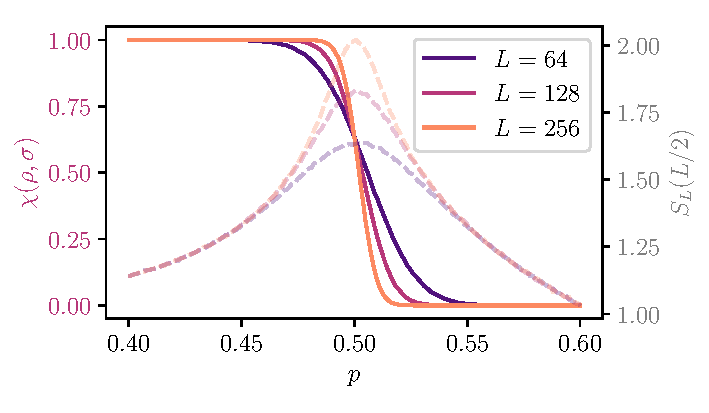
\includegraphics{simple_lxe_ptim_three_sizes_circuits.pdf}
  \caption{Let's see if the colormap synergizes with the rest of the layout. I
  sure do hope so.}
  \label{fig:firstattempt-lxe}
\end{figure}

\Cref{fig:err-vs-tra} hopefully looks nice. Maybe it also floats to the correct
place!
\begin{figure}[h]
  \centering
  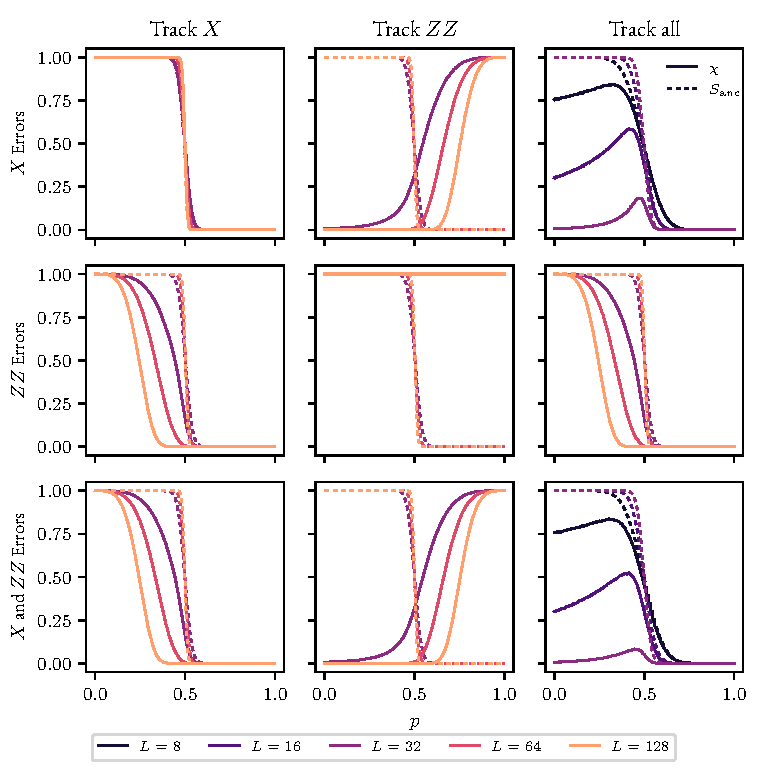
\includegraphics{errors-vs-tracked.pdf}
  \caption{Which measurement outcomes have been tracked and used to compute the
  linear cross entropy, vs the type of errors simulated.}
  \label{fig:err-vs-tra}
\end{figure}
It didn't seem to do so, so i passed \texttt{[h]}
\lipsum[0-2]
Nielsen \cite{nielsenQuantumComputationQuantum2010} Gottesman
\cite{gottesmanStabilizerCodesQuantum1997}
\cite{aaronsonImprovedSimulationStabilizer2004}
\section{WOAH!}
\lipsum[3]
entropy in stabilizer formalism
\cite{fattalEntanglementStabilizerFormalism2004}
ptim nicolai \cite{langEntanglementTransitionProjective2020}
\subsection{Coole Subsection}
\lipsum[4-6]
\cite{roserDecodingProjectiveTransverse2023}
\subsubsection{Coole Subsubsection}
\lipsum[7-9]
\subsubsection{Dies ist ein Test!}
\lipsum[10-11]
\subsection{Noch ein Test!}
\lipsum[12-14]
\cite{tikhanovskayaUniversalityCrossEntropy2023}
\section{Neue Section mit mehreren Equations aus der BA}
Diese Section ist geklaut aus meiner BA. Da dort ein paar wilde Mathesachen
vorkommen, dachte ich dass es vielleicht ein guter Test ist sowohl für Layout
als auch Typeface.

In classical Hamiltonian mechanics the state of a system (at some time $t$) is
represented by a point $\xi$ in phase space, which, for a system with $n$
degrees of freedom, resides in $\mathbb{R}^{2n}$
\cite{noltingHamiltonMechanik2014}.\\
According to the first postulate of quantum mechanics, the state of a system
(at time $t$) is defined by a unit vector in Hilbert space $\mathcal{H}$,
called \emph{state vector} \cite{cohen-tannoudjiQuantumMechanicsVolume1977}.
This gives rise to an
intriguing fundamental difference to the classical world, since any arbitrary
vector (in $\mathcal{H}$) can be represented as a linear combination of basis
vectors.  This is called the superposition principle
\cite{poschelFourierreihen2015, messiahQuantumMechanics1991}.
Let us consider the fundamental example of a two-state system, with a ground state '0' and an excited state '1'.
Note that in the context of quantum information this type of system is referred to as \emph{qubit}.
The most general state of the system is described by a superposition of the two states,  
\begin{align}\label{eq:superpos}
    \ket{\psi} = c_1 \ket{0} + c_2 \ket{1}.
\end{align}
In \cref{eq:superpos}, quantum states are represented using the so-called Bra-Ket-notation. 
The state vector of a quantum system in $\mathcal{H}$ is denoted by $\ket{\psi}$\footnote{read: Ket $\psi$. Also called \emph{Ket-vector}},
with the corresponding vector $\bra{\psi}$\footnote{read: Bra $\psi$. Also called \emph{Bra-Vector}} in dual space.
The inner product on $\mathcal{H}$ is then defined as
$\braket{\varphi}{\psi}$.
\par
Since states are elements of a complex vector space, they are not physical observable quantities. Therefore, the formalism
has to be complemented with a mathematical formalism of observables in order to get a complete and meaningful description of quantum systems.
In general, physical quantities can be measured (observed) and the outcome of such a measurement should therefore be
a real\footnote{as opposed to complex} number.
For this we employ the second postulate of quantum mechanics. It states that measureable physical quantities
(observables) are Hermitian operators acting in $\mathcal{H}$. 
The Hermitian property implies that the operator only has real eigenvalues, is diagonalizable,
and that its eigenvectors are orthogonal \cite{messiahQuantumMechanics1991}.\\
%We measure by applying an operator of an observable $\hat{A}$ to the state vector $\ket{\psi(t)}$ is called measuring.
Let us convince ourselves of the advantages that come with this Hermitian property.
Suppose we want to measure some observable $A$.
The outcome of such a measurement is an eigenvalue $a_k$ of the operator $\hat{A}$. The probability to observe the specific outcome $a_k$ is
\begin{align}\label{eq:prob-meas}
    p(a_k) = \braket{\psi}{a_k}\braket{a_k}{\psi} = \abs{\braket{a_k}{\psi}}^2,
\end{align}
where $\bra{a_k}$ are the eigen-bras of $\hat{A}$ with eigenvalue $a_k$.\\
Due to the inherent probabilistic description of quantum mechanics (cf. \cref{eq:prob-meas}), we can only make meaningful statements about averages.
Weighing every eigenvalue $a_k$ with its respective probability to be measured
given by \cref{eq:prob-meas}, the average of an observable becomes
\cite{nielsenQuantumComputationQuantum2010}
\begin{align}
    \expval{\hat{A}} = \sum\limits_k a_k p(a_k) = \sum\limits_k a_k \braket{\psi}{a_k}\braket{a_k}{\psi}
    = \bra{\psi} \left(\sum\limits_k a_k \dyad{a_k}\right) \ket{\psi} = \ev{\hat{A}}{\psi}.
\end{align}\\
Let us consider a concrete example of an operator.
Arguably the most essential operator in quantum mechanics is the Hamilton operator $\hat{H}$, often simply abbreviated as Hamiltonian.
It describes the total energy of a system, and is the generator of time translation, i.e. time evolution. A state vector evolves
according to the \emph{Schrödinger equation}, defined as
\cite{messiahQuantumMechanics1991}
\begin{align}\label{eq:schro-eq}
    i\partial_t \ket{\psi(t)} = \hat{H} \ket{\psi(t)}.
\end{align}
Solving \cref{eq:schro-eq} gives us
\begin{align}\label{eq:schro-sol}
    \ket{\psi(t)} = e^{-i\hat{H}t}\ket{\psi(0)} \equiv U(t)\ket{\psi(0)}
\end{align}
with $U(t)$ defined as the unitary time evolution operator. Unitary operators fulfil the relation $UU^\dagger=\mathds{1}$, i.e.
its inverse is given by its Hermitian conjugate. Using the fact that the Hamiltonian is a Hermitian operator, unitarity follows from 
\begin{align}\label{eq:unitary-property}
    U(t)U^\dagger(t) = e^{-i\hat{H}t}e^{i\hat{H}^\dagger t} = e^{-i\hat{H}t}e^{i\hat{H}t} = \mathds{1}.
\end{align}
The determinant of such an operator is $1$, meaning that
the state vector the operator acts upon keeps unit length during its time evolution.
\par
In \cref{eq:schro-sol} and \cref{eq:unitary-property} we used the exponential of an operator. Since the
product of operators and
the series expansion of the exponential function are well defined, the exponential of an operator is defined through series expansion.
For instance, the series expansion of $U(t)$ becomes
\begin{align}\label{eq:matrix-exp}
    U(t) = \sum\limits_{n=0}^\infty \frac{(-i\hat{H}t)^n}{n!}.
\end{align}




\appendix

\chapter{Code Listings}
\label{ch:apdx-code}

\lstset{style=myStyle}

\verb|C++| code for the computation of $\chi_C$.
\begin{lstlisting}[caption=Computation of the linear cross entropy for one
  measurement history of a circuit, label={lst:lxe-cpp}, language=C++]
bool success = true; 
for (int t=0; t<t_max; t++) {
    for (int s=0; s<L; s++) {
        if (random_circuit_x[t][s] && success) {
           success = P.project(X,s,measurements_x[t][s]);
        }
    }
    for (int s=0; s<L-1; s++){
        if (random_circuit_zz[t][s] && success) {
           success = P.project(Z,s,Z,periodic(s+1,L),measurements_zz[t][s]);
        }
    }
}
if (success) {
results.lxs.av++;
results.lxs.se++;
}
\end{lstlisting}

\verb|C++| code for the \verb|entropy_vn| function, computing the von Neumann
entropy.
\begin{lstlisting}[caption=\texttt{entropy\_vn} function in the simulator,
label={lst:entropy-vn-cpp}, language=C++]
int Qubits::entropy_vn() {
    return mix;
}
\end{lstlisting}

\verb|C++| code for the \verb|is_subgroup_of| function.
\begin{lstlisting}[caption=\texttt{is\_subgroup\_of} function in the simulator,
label={lst:is-subgroup-of-cpp}, language=C++]
      bool Qubits::is_subgroup_of(Qubits& other) {
          if (other.N != N || other.mix > mix) return false;


          // Signs
          BYTE* comb_r = new BYTE[(2*N+1+7)/8];

          for (int i=0; i<(2*N+1+7)/8; i++)
              comb_r[i] = 0;

          for (int g = 0; g<N-other.mix; g++) {
              set_bit(comb_r,g,get_bit(other.r,2*g));
          }
          for (int g = N; g<2*N-mix; g++) {
              set_bit(comb_r,g,get_bit(this->r,2*(g-N)));
          }


          // Table
          int Nb = (2*N+1+7)/8; // N X stabilizer, N Z stabilizer

          BYTE* loc_buf = new BYTE[2*N*Nb];
          for (int i=0; i<2*N*Nb; i++) loc_buf[i]=0;
          // 2N rows, since we're comparing two stabilizer matrices
          BYTE** local = new BYTE*[2*N];
          for (int r=0; r<2*N; r++) {
              local[r] = loc_buf+Nb*r;
          }
          for (int i=0; i<2*N; i++) {
              for (int j=0; j<((2*N+1)+7)/8; j++)
                  local[i][j] = 0;
          }

          for (int c=0; c<N; c++) { // fill columns
              for (int r=0; r<N-other.mix; r++) { // fill rows 1-N with other
                  set_bit(local[r],2*c,other.has(X,c,2*r));
                  set_bit(local[r],2*c+1,other.has(Z,c,2*r));
              }
              for (int r=N; r<2*N-mix; r++) { // fill rows N+1-2N with this
                  set_bit(local[r],2*c,this->has(X,c,2*(r-N)));
                  set_bit(local[r],2*c+1,this->has(Z,c,2*(r-N)));
              }
          }


            int R=0;
            for (int c=0; c<2*N; c++) {

#if DEBUG_ES
                /* print_bit_matrix(local,N,2*n); */
#endif

                // Find pivot
                bool pivot = true;
                for (int r=R; r<2*N; r++) {
                    if (get_bit(local[r],c)) {
                        // Swap pivot to top
                        if (pivot && r<N) {
                            swap_rows(local,R,r);
                            swap_bits(comb_r,R,r);
                            pivot = false;
                        }
                        // pivot should never be on the bottom,
                        // since it is then no longer a subgroup
                        else if (pivot && r>=N) {
                            return false;
                        }
                        // Zero column below pivot
                        else {
                            add_row_to(local,Nb,R,r);
                            // XOR the bit at position r in comb_r[r] with the bit at position R in comb_r[R]
                            comb_r[r / 8] ^= ((comb_r[R / 8] >> (R % 8)) & 1) << (r % 8);
                        }
                    }
                }
                if (!pivot) R++;
            }
            // check that there is no hanging sign anywhere
            // This would be the case if the groups matched perfectly up to
            // sign differences
            for (int i=N; i<2*N-mix; i++) {
                if (get_bit(comb_r, i)) return false;
            }

            return true;


            delete[] comb_r;
            delete[] local;
            delete[] buf;

      }
\end{lstlisting}

\verb|C++| code for the \verb|cross_entropy| function.
\begin{lstlisting}[caption=\texttt{cross\_entropy} function in the simulator,
label={lst:cross-entropy-cpp}, language=C++]
double Qubits::cross_entropy(Qubits& other) {
    if (!(this->is_subgroup_of(other))) return std::numeric_limits<double>::quiet_NaN();
    else return (double) mix;
}
\end{lstlisting}

\verb|C++| code for the \verb|relative_entropy| function.
\begin{lstlisting}[caption=\texttt{relative\_entropy} function in the simulator,
label={lst:relative-entropy-cpp}, language=C++]
double Qubits::relative_entropy(Qubits& other) {
    if (!(this->is_subgroup_of(other))) return std::numeric_limits<double>::quiet_NaN();
    else return (double) mix - other.mix;
}
\end{lstlisting}

\verb|C++| code for the \verb|get_state_type| function.
\begin{lstlisting}[caption=\texttt{get\_state\_type} function in the simulator,
label={lst:get-state-type-cpp}, language=C++]
int Qubits::get_state_type(const int q) {
    int dummy{}, val{};
    for ( int i = 0; i < 2*(N-mix); i+=2 ) {
        val = 2*get_bit(tab[q],2*i)+get_bit(tab[q],2*i+1);
        if ( val != 0 && dummy == 0 ) dummy = val;
        else if ( val != 0 && val != dummy ) return 1;
    }
    if (dummy) return 0;
    else return -1;
}
\end{lstlisting}
\verb|C++| code for the \verb|rowreduce| function.
\begin{lstlisting}[caption=\texttt{rowreduce} function in the simulator,
label={lst:rowreduce-cpp}, language=C++]
void Qubits::rowreduce(const int q) {
   // helper variables
   int first_x = -1, first_z = -1;
   int num_x{}, num_z{};
   int last_stab = 2*(N-1), last_anti = 2*N-1;

   // loop through x stabilizer
   for (int j = 0; j < 2*N; j += 2) {
       if ( get_bit( tab[q], 2*j ) && num_x == 0 ) {
           first_x = j;
           num_x++;
       }
       else if ( get_bit( tab[q], 2*j ) && num_x > 0 ) {
           rowsum(j,first_x);             // update stabilizer
           rowsum(first_x+1, j+1);     // update antistabilizer in parallel
           num_x++;
       } 
   }

   if ( num_x > 0 && first_x != last_stab ) {
       for (int k = first_x; k<last_stab; k++){
           rowswap(k,k+2);
       }
   }


   // loop through z stabilizer
   for (int j = 0; j < 2*N; j += 2) {
       if ( get_bit( tab[q], 2*j+1 ) && num_z == 0 ) {
           first_z = j;
           num_z++;
       }
       else if ( get_bit( tab[q], 2*j+1 ) && num_z > 0 ) {
           rowsum(j,first_z);             // update stabilizer
           rowsum(first_z+1,j+1);     // update antistabilizer in parallel
           num_z++;
       } 
   }


   if ( num_z > 0 && ((num_x > 0 && first_z != last_stab) || num_x==0)) {
       for (int k = first_z; k<last_stab; k++){
           rowswap(k,k+2);
       }
   }

}
\end{lstlisting}


\chapter{Fragments and Tangents}
\label{ch:fragments}

\section{On tangents}
While writing this thesis my thoughts have wandered off once or twice. Almost
always while writing out something completely different. Incidentally, this is
how the paragraph you're reading right now came to be.

Sometimes I'd write down something that amuses me, sometimes I'd get frustrated
and investigate my frustrations in text. Maybe I had even had a profound
thought once in a while.  Regardless of how these tangents got there, or what
they are about, off-topic tangents are not something you'll want to put in the
main body of your thesis, no matter how ingqnious or witty they are.  Come to
think of it, they probably do not belong in the appendix either.

Either way, I would have been quite distraught to delete these paragraphs
without any of them seeing the inside of a printer. So, in order for them not
to go to waste, I decided to collect them here for mine and my friends'
amusement. These texts really are silly sometimes.

\section{On references}
I like how references are provided in physics: all those little numbers in
little brackets or as superscript above a claim to support it. It allows me to
follow the bibliography in parallel to the paper and check some pertinent
publications easily. This is, of course, very different in many other
disciplines, e.g. psychology or philosophy, where it is common-practice to give
your sources in alphabetical order sorted by the author's surname.

I claim that physicists are not appreciative enough of this. It will never fail
to frustrate me if people cite some shit that has nothing at all to do with the
claim in question. This is especially so if the claim is better supported by
the results of other papers; papers that a lot of times make it into the
\texttt{.bib} file of at least one of the authors, or why else would they be
prominently cited in a section, where it doesnt make sense to do so.
Ultimately, the highest degree of frustration for me is if the references are
off by one, or cite a previous project by the same authors. This kind of
situation lies in the uncanny valley of "is it them or me?". And more often
than not, it should be \emph{me}, right? But then you go on and on, read the
cited papers thoroughly, try to understand the context in which it is
referenced in the work you originally went through, and now, multiple layers
deep in the reference rabbithole are you ultimately forced to realize that it's
not you, it's them. 



\backmatter

\chapter{Acknowledgements}
\label{ch:ack}
\epigraph{Whoever claims to love God yet hates a brother or sister is a liar.
  For whoever does not love their brother and sister, whom they have seen,
cannot love God, whom they have not seen.}{
1 John 4:20}
\lipsum[1]


\cleardoublepage
\addcontentsline{toc}{chapter}{Bibliography}
{\footnotesize\printbibliography}

\end{document}
